%%
%% This is file `sample-sigconf.tex',
%% generated with the docstrip utility.
%%
%% The original source files were:
%%
%% samples.dtx  (with options: `all,proceedings,bibtex,sigconf')
%% 
%% IMPORTANT NOTICE:
%% 
%% For the copyright see the source file.
%% 
%% Any modified versions of this file must be renamed
%% with new filenames distinct from sample-sigconf.tex.
%% 
%% For distribution of the original source see the terms
%% for copying and modification in the file samples.dtx.
%% 
%% This generated file may be distributed as long as the
%% original source files, as listed above, are part of the
%% same distribution. (The sources need not necessarily be
%% in the same archive or directory.)
%%
%%
%% Commands for TeXCount
%TC:macro \cite [option:text,text]
%TC:macro \citep [option:text,text]
%TC:macro \citet [option:text,text]
%TC:envir table 0 1
%TC:envir table* 0 1
%TC:envir tabular [ignore] word
%TC:envir displaymath 0 word
%TC:envir math 0 word
%TC:envir comment 0 0
%%
%% The first command in your LaTeX source must be the \documentclass
%% command.
%%
%% For submission and review of your manuscript please change the
%% command to \documentclass[manuscript, screen, review]{acmart}.
%%
%% When submitting camera ready or to TAPS, please change the command
%% to \documentclass[sigconf]{acmart} or whichever template is required
%% for your publication.
%%
%%
\documentclass[sigconf]{acmart}
\settopmatter{printacmref=false}  % hides ACM Reference Format block
\setcopyright{none}               % hides DOI/ISBN/conference line
\acmConference[]{}{}{}            % clears conference info
\acmBooktitle{}                   % clears book title
\acmPrice{}                       % clears price
\acmISBN{}                        % clears ISBN
\acmDOI{}                         % clears DOI
\pagestyle{plain}                 % optional: removes running headers

\usepackage{tabularx,makecell,ragged2e,booktabs}
\newcolumntype{L}[1]{>{\RaggedRight\arraybackslash}p{#1}}
\newcolumntype{Y}{>{\RaggedRight\arraybackslash}X}
\renewcommand\theadfont{\bfseries}

\usepackage{float}
\usepackage{placeins}

\usepackage{booktabs}        % for \toprule, \midrule, 
\usepackage{makecell}        % for \thead
\usepackage{threeparttable} 
\usepackage{placeins}

\usepackage{titlesec}
% Reduce spacing before/after subsections
\titlespacing*{\subsection}{0pt}{0.7ex plus .2ex}{0.3ex}

\usepackage{enumitem}
% Make bullet lists compact
\setlist[itemize]{topsep=2pt, itemsep=2pt, parsep=0pt, partopsep=0pt}


%%
%% \BibTeX command to typeset BibTeX logo in the docs
\AtBeginDocument{%
  \providecommand\BibTeX{{%
    Bib\TeX}}}

%% Rights management information.  This information is sent to you
%% when you complete the rights form.  These commands have SAMPLE
%% values in them; it is your responsibility as an author to replace
%% the commands and values with those provided to you when you

%% complete the rights form.
\begin{comment}
\setcopyright{acmlicensed}
\copyrightyear{2018}
\acmYear{2018}
\acmDOI{XXXXXXX.XXXXXXX}
%% These commands are for a PROCEEDINGS abstract or paper.
\acmConference[Conference acronym 'XX]{Make sure to enter the correct
  conference title from your rights confirmation email}{June 03--05,
  2018}{Woodstock, NY}
%%
%%  Uncomment \acmBooktitle if the title of the proceedings is different
%%  from ``Proceedings of ...''!
%%
%%\acmBooktitle{Woodstock '18: ACM Symposium on Neural Gaze Detection,
%%  June 03--05, 2018, Woodstock, NY}
\acmISBN{978-1-4503-XXXX-X/2018/06}
\end{comment}


%%
%% Submission ID.
%% Use this when submitting an article to a sponsored event. You'll
%% receive a unique submission ID from the organizers
%% of the event, and this ID should be used as the parameter to this command.
%%\acmSubmissionID{123-A56-BU3}

%%
%% For managing citations, it is recommended to use bibliography
%% files in BibTeX format.
%%
%% You can then either use BibTeX with the ACM-Reference-Format style,
%% or BibLaTeX with the acmnumeric or acmauthoryear sytles, that include
%% support for advanced citation of software artefact from the
%% biblatex-software package, also separately available on CTAN.
%%
%% Look at the sample-*-biblatex.tex files for templates showcasing
%% the biblatex styles.
%%

%%
%% The majority of ACM publications use numbered citations and
%% references.  The command \citestyle{authoryear} switches to the
%% "author year" style.
%%
%% If you are preparing content for an event
%% sponsored by ACM SIGGRAPH, you must use the "author year" style of
%% citations and references.
%% Uncommenting
%% the next command will enable that style.
%%\citestyle{acmauthoryear}

\usepackage{tikz}
\usetikzlibrary{arrows, positioning, shapes.geometric, calc}

%%
%% end of the preamble, start of the body of the document source.
\begin{document}

% --- keep sigconf, but hide all ACM metadata/footers ---
\settopmatter{printacmref=false}
\setcopyright{none}

% clear anything that could still render a stub
\acmConference[]{}{}{}
\acmBooktitle{}
\acmPrice{}
\acmISBN{}
\acmDOI{}
\acmYear{}
\copyrightyear{}


% remove the permission footnote AND the horizontal rule above it
\makeatletter
\renewcommand\footnotetextcopyrightpermission[1]{} % kills the copyright footnote text
\renewcommand{\footnoterule}{}                      % kills the thin rule above footnotes
\makeatother


\pagestyle{plain}  % optional (no running headers)


%%
%% The "title" command has an optional parameter,
%% allowing the author to define a "short title" to be used in page headers.
\title{Group 02: A Study on Performance and Parameter Sensitivity of Flash Cache Eviction Policies Using BCacheSim on Production Baleen Traces}

%%
%% The "author" command and its associated commands are used to define
%% the authors and their affiliations.
%% Of note is the shared affiliation of the first two authors, and the
%% "authornote" and "authornotemark" commands
%% used to denote shared contribution to the research.
\author{Behab Patnaik}
\email{b.patnaik@student.fdu.edu}
\affiliation{%
  \institution{Fairleigh Dickinson University}
  \city{Vancouver}
  \state{British Columbia}
  \country{Canada}
}


\author{Khaja Aweas Mohiuddin}
\email{k.mohiuddin@student.fdu.edu}
\affiliation{%
  \institution{Fairleigh Dickinson University}
  \city{Vancouver}
  \state{British Columbia} 
  \country{Canada}
  }
\author{Abdur Rahman}
\email{a.rahman6@student.fdu.edu}
\affiliation{%
  \institution{Fairleigh Dickinson University}
  \city{Vancouver}
  \state{British Columbia}
  \country{Canada}
  }

\author{Mahjabeen Naaz}
\email{m.naaz@student.fdu.edu}
\affiliation{%
  \institution{Fairleigh Dickinson University}
  \city{Vancouver}
  \state{British Columbia}
  \country{Canada}
  }

\author{Thabassum Thabassum}
\email{t.thabassum@student.fdu.edu}
\affiliation{%
  \institution{Fairleigh Dickinson University}
  \city{Vancouver}
  \state{British Columbia}
  \country{Canada}
  }


%%
%% By default, the full list of authors will be used in the page
%% headers. Often, this list is too long, and will overlap
%% other information printed in the page headers. This command allows
%% the author to define a more concise list
%% of authors' names for this purpose.
\renewcommand{\shortauthors}{Trovato et al.}

%%
%% The abstract is a short summary of the work to be presented in the
%% article.
\begin{comment}
\begin{abstract}
  A clear and well-documented \LaTeX\ document is presented as an
  article formatted for publication by ACM in a conference proceedings
  or journal publication. Based on the ``acmart'' document class, this
  article presents and explains many of the common variations, as well
  as many of the formatting elements an author may use in the
  preparation of the documentation of their work.
\end{abstract}
\end{comment}

%%
%% The code below is generated by the tool at http://dl.acm.org/ccs.cfm.
%% Please copy and paste the code instead of the example below.
%%

\begin{comment}
\begin{CCSXML}
<ccs2012>
 <concept>
  <concept_id>00000000.0000000.0000000</concept_id>
  <concept_desc>Do Not Use This Code, Generate the Correct Terms for Your Paper</concept_desc>
  <concept_significance>500</concept_significance>
 </concept>
 <concept>
  <concept_id>00000000.00000000.00000000</concept_id>
  <concept_desc>Do Not Use This Code, Generate the Correct Terms for Your Paper</concept_desc>
  <concept_significance>300</concept_significance>
 </concept>
 <concept>
  <concept_id>00000000.00000000.00000000</concept_id>
  <concept_desc>Do Not Use This Code, Generate the Correct Terms for Your Paper</concept_desc>
  <concept_significance>100</concept_significance>
 </concept>
 <concept>
  <concept_id>00000000.00000000.00000000</concept_id>
  <concept_desc>Do Not Use This Code, Generate the Correct Terms for Your Paper</concept_desc>
  <concept_significance>100</concept_significance>
 </concept>
</ccs2012>
\end{CCSXML}

\ccsdesc[500]{Do Not Use This Code~Generate the Correct Terms for Your Paper}
\ccsdesc[300]{Do Not Use This Code~Generate the Correct Terms for Your Paper}
\ccsdesc{Do Not Use This Code~Generate the Correct Terms for Your Paper}
\ccsdesc[100]{Do Not Use This Code~Generate the Correct Terms for Your Paper}
\end{comment}

%%
%% Keywords. The author(s) should pick words that accurately describe
%% the work being presented. Separate the keywords with commas.
\begin{comment}
\keywords{Do, Not, Use, This, Code, Put, the, Correct, Terms, for,
  Your, Paper}
%% A "teaser" image appears between the author and affiliation
%% information and the body of the document, and typically spans the
%% page.
\begin{teaserfigure}
  \includegraphics[width=\textwidth]{sampleteaser}
  \caption{Seattle Mariners at Spring Training, 2010.}
  \Description{Enjoying the baseball game from the third-base
  seats. Ichiro Suzuki preparing to bat.}
  \label{fig:teaser}
\end{teaserfigure}

\received{20 February 2007}
\received[revised]{12 March 2009}
\received[accepted]{5 June 2009}
\end{comment}

%%
%% This command processes the author and affiliation and title
%% information and builds the first part of the formatted document.


\begin{abstract}
Flash caching plays an important role to reduce disk head time DT in storage systems, because when the disk head moves too much it will slow the application performance. Some common eviction policies like LRU, DT SLRU, and EDE are used for this purpose, but they often need tuning to make a good balance. In this work, we use BCacheSim to test these three policies in different cache configurations, and study how changing important parameters affect the performance. The parameters we check include protected capacity, tau DT threshold, and alpha TTI rate.

From the experiments, we notice that tuning alpha TTI to around 0.15 gives large improvement. The peak DT goes down from about 4.91 second to 3.38 second, which is almost 31 percent better. Another parameter, protected capacity around 0.45, also reduce peak DT from near 4.18 second to about 3.75 second, close to 10 percent improvement. When we compare the baseline performance, LRU shows peak DT of 3.03 second, while DT SLRU gives around 3.97 second and EDE is near 4.16 second. This result shows that no single policy is best always. Good performance needs careful tuning for each workload, and different policies require different tuning strategies to reduce disk head time and keep cache hit rate stable.
\end{abstract}

\maketitle

\clearpage
\section{Introduction}
Many storage systems today use flash cache in front of slower hard disks to answer requests faster. This helps when many users access data, but performance is not always good. Sometimes the cache fills with data not used again, wasting space and pushing out useful items. When this happens, the system becomes slower. In this study we look at how to choose which data to admit and which to evict. The goal is to reduce disk head time while keeping a good hit rate and also avoid too much writing on flash in real overall system performance in practical use.

In this study we look at simple cache policies like LRU and also more advanced policies such as DT SLRU and EDE. We also consider a machine learning admission system called Baleen \cite{wong2024baleen}. These different systems all try to deal with the problem of objects that sometimes get popular for a short time and then not used anymore. The system designer has to choose parameters like how much part of the cache to protect, or how fast to adapt to new patterns. \cite{Yang2022CacheSack}.

There are three main families of solutions people use before. The first family has simple eviction policies like LRU or FIFO. These policies accept everything and then later decide what to throw away. They are simple but they write a lot of unnecessary things to flash because they store many items that will only be used once. This increases write traffic and also causes useful items to get removed earlier. The second family tries to combine recency and heuristics that match storage device behavior, for example DT SLRU. Here a part of the cache is for objects that already showed some reuse. The third family treats admission as a prediction problem. EDE looks at how long an object stays idle and tries to detect episodes of popularity.  

Because each of these families have strengths and weaknesses, we decide to create a complete evaluation method using BCacheSim. This simulation tool allows us to test the policies side by side under the same conditions. We test them using traces that are similar to real system behavior. We look at metrics like hit rate, peak disk head time, median disk head time, and how much write traffic happens to flash. 

One important design in our work is that we focus strongly on disk head time rather than only hit rate. Hit rate is a common measurement but sometimes two configurations can have similar hit rates but very different disk head time. This happens because when misses happen at different times it affects how busy the backend disk gets. Peak disk head time is very important in multi user systems because when the backend is too busy, the latency becomes very high.

From our results we find three important patterns. First, the strictness of admission must match how bursty the workload is. In our alpha\_TTI experiment, we found that if the adaptation is too fast, the system becomes noisy and performance becomes worse. But with a medium setting around 0.15, peak disk head time improved a lot, lowering from around 4.91 to 3.38 which is around 31 percent improvement. Hit rate also improved and the amount of flash writing went down at the same time. Second, adding more segmentation improves noise filtering but only until a certain point. In experiments where we increase the protected region, the peak disk head time decreased at first. But after the protected part got too large, the improvement disappeared and performance sometimes even became worse, because new items could not move into the protected part easily. Third, LRU is surprisingly strong on the traces we tested. LRU got around 3.03s peak DT which was better than DT SLRU and EDE which got around 3.97s and 4.16s respectively. But when we tune parameters carefully, the other policies come closer to LRU but with better control of write traffic. \cite{Yang2022CacheSack}.

One reason previous approaches alone are not enough is that flash endurance and write amplification are real limitations. If we write too much to flash it wears out faster. So we must select items carefully \cite{Yang2022CacheSack}. Also many storage systems use compression or deduplication and that adds overhead that has to be considered \cite{Wang2020AustereCache}. Different workloads have different locality patterns so a good parameter setting for one system might be bad for another. 

Our framework helps this by combining everything in one pipeline. We use the simulate\_ap driver in BCacheSim to replay traces. We created structured configuration files that store all information for each run. The results are stored in directories that allow easy aggregation later. We have figure scripts that take the output, calculate medians and peaks, and make plots with labels. 

We also include episodic analysis. Many misses happen because an object's popularity is changing. EDE and Baleen try to use this by capturing when episodes start or end \cite{wong2024baleen}. Our pipeline allows calculating how often we admit things at the start of an episode or whether the admission was useful later. 

We also keep in mind that systems must operate under real constraints like flash write limits and interactions with other components like prefetching. So we do not only show hit rate. We also show how many writes occur. For example in the tau\_DT test we saw that if the threshold is too permissive, the system writes more but does not get better disk head time. But if the threshold is too strict, good items might be refused. Real deployments therefore adjust parameters slowly and not rapidly every moment \cite{Yang2022CacheSack}.

In conclusion, our project gives a careful study of cache admission and eviction strategies for flash caching in storage systems. We show that tuning alpha\_TTI and protected capacity can reduce peak disk head time a lot. We also show that LRU is still very strong in many situations but policies with episodic or learned ideas can provide better stability for writes and can react better when signals are strong \cite{wong2024baleen}.Following are some contributions that our project makes.
\begin{itemize}
    \item We made one evaluation setup using BCacheSim so other people can repeat our tests. It puts all traces, cache policies like LRU, DT SLRU, EDE and Baleen, and also the measurement numbers like peak DT, median DT, hit rate and flash write amount in one place. 

    \item We tested how changing three main settings affect the results. These settings are how much cache space is protected, the tau\_DT value, and the alpha\_TTI rate. Changing alpha\_TTI gave around 31 percent lower peak DT. Changing protected capacity gave around 10 percent better DT. 

    \item We found the ranking of the policies in our traces. LRU had the lowest peak DT which was about 3.03 seconds. But when we tuned the episodic and learned admission methods, they came close to LRU and also used flash more carefully so they had better stability in some cases.

\end{itemize}

\clearpage
\section{Background}
This section provides the technical background necessary to understand our evaluation of cache eviction policies for flash caching in storage systems.

\subsection{Flash Caching in Storage Systems}
Modern systems usually put a flash cache between RAM and the slow disk so the requests can finish faster \cite{wong2024baleen, Yang2022CacheSack}. The system checks RAM first, then flash, and only then the backend. When flash has the data it avoids a slow disk read and this makes the latency smaller and also reduces pressure on the backend \cite{Oh2010CachingLess}. But flash cannot handle too many writes because the chips get worn out, and garbage collection makes even more writes than expected \cite{Wang2020AustereCache}. So the cache needs careful management to not damage the flash too fast.

The cache manager mainly decides what to admit and what to evict. Bad choices lower hit rate and increase latency and even produce too many writes \cite{li2016cachededup, shen2016cloudcache}. Workloads keep changing. Sometimes an item is reused soon which is temporal locality, and sometimes it becomes very hot only for a short episode and then it is not used again. Good policies try to handle these patterns while still protecting the flash \cite{mcallister2024fairywren, lerasle2015emrc, liu2020maperx}.

\subsection{Cache Eviction Policies}
LRU is a very common idea where the cache throw out the item that was not touched for the longest time, and it keeps everything in one order that follow how recently things were used \cite{Oh2010CachingLess}. When there is a miss it just removes the item that stay in the front of this order. Because of this simple rule the behavior is kind of easy to guess and it works pretty ok when the workload has strong time pattern \cite{lerasle2015emrc}. But it also has some problems because it treats all objects like they are same even when they are not, so it never think about if an item is big or small or if writing it will cost a lot on the flash device \cite{liu2020maperx}. In flash caching this is not so good because some blocks that have very high disk head time actually get more benefit when they stay in the cache, but LRU do not give any special focus to them and many time it just evicts them like everything else \cite{wong2024baleen}. These weaknesses become especially clear when compared with DT-aware or episodic-aware structures such as those shown in Figure~\ref{fig:dtslru_structure} and Figure~\ref{fig:ede_episodes} \cite{Yang2022CacheSack}.

DT SLRU tries to improve normal LRU by using disk head time and by splitting the cache into probation and protected parts~\cite{wong2024baleen}. New blocks always begin in probation and only move to protected when they show enough value, usually after two hits or when their DT per byte score is higher than $\tau_{\mathrm{DT}}$~\cite{Yang2022CacheSack}. Inside the protected area the blocks still follow LRU order, and eviction starts from probation first. The $\tau_{\mathrm{DT}}$ value controls how strict the promotion is, since low values let many blocks enter and high values only allow a few. This parameter changes the cache shape and affects performance. The main goal is to keep higher value blocks safe while still following temporal order~\cite{Oh2010CachingLess}, as shown in Figure~\ref{fig:dtslru_structure} and compared with episodic behavior in Figure~\ref{fig:ede_episodes}~\cite{mcallister2024fairywren}.


EDE tries to deal with items that become popular only for a short time and then fade, and it guesses when this episode is ending by checking things like the biggest time gap between two accesses~\cite{wong2024baleen}. The cache has two parts, a protected area for items with high DT per byte and an unprotected area for the normal ones~\cite{Yang2022CacheSack}. An item only moves to protected when its DT per byte or its episode pattern look strong enough, as illustrated in Figure~\ref{fig:ede_episodes}.

There is a protected cap that controls how much space this section can use, and choosing too big or too small can block new items or push out valuable ones~\cite{Oh2010CachingLess}. EDE also updates the time to idle using an EWMA with $\alpha_{\mathrm{TTI}}$, where small $\alpha_{\mathrm{TTI}}$ change slowly and big $\alpha_{\mathrm{TTI}}$ change too fast~\cite{mcallister2024fairywren}. EDE is good for episodic popularity, but if the prediction is wrong it can evict things too early or keep them longer than needed, which becomes clear when comparing with DT-aware structures in Figure~\ref{fig:dtslru_structure}.

\subsection{Disk Head Time and Service Time Metrics}
Disk head time, or DT, is how long the disk head stays busy doing seeks and transfers \cite{wong2024baleen}. When many disks run together this time can grow a lot. Service time is how long the backend needs to finish a request and it mainly comes from the seek, the rotation wait, and the data move \cite{Yang2022CacheSack}. In this work it is modeled by multiplying the I O count with $T_{\mathrm{seek}}$ and adding the chunk transfer using chunk size and bandwidth. Here $T_{\mathrm{seek}}$ is around 11.5 ms and the bandwidth is around 143 MB/s. These DT ideas also help show why DT based designs in Figure~\ref{fig:dtslru_structure} act different from episodic ones in Figure~\ref{fig:ede_episodes}.

Peak DT is the highest DT in a window and shows the worst delay \cite{Oh2010CachingLess}. Median DT is the usual case since it ignores spikes. Hit rate only shows how many hits happened but two systems can have same hit rate and very different DT \cite{mcallister2024fairywren}. So DT is many times a clearer way to compare cache behavior.


\subsection{BCacheSim and Episodic Analysis}
BCacheSim is a small Python tool that replays real storage traces so we can test different flash cache rules~\cite{wong2024baleen}. It has one part that reads the trace and one simple cache simulator that uses the policies we choose like LRU, DT SLRU, EDE, Baleen, AcceptAll and some others~\cite{Yang2022CacheSack}. The data is cut in fixed chunks around 128\,KB. We set the experiment with a JSON file where we put cache size and a few parameters like $\tau_{\mathrm{DT}}$ or PROTECTED cap. After it runs, it gives a JSON result with basic numbers like hit rate and service time. The basic behaviors of DT-based and episodic policies can also be matched to the layouts shown in Figure~\ref{fig:dtslru_structure} and Figure~\ref{fig:ede_episodes}.

The tool also try to study something called episodes. An episode is when one item gets active for some time and then it becomes quiet, and many misses happen when the item was removed during the quiet part~\cite{Oh2010CachingLess}. Policies like EDE use interarrival time patterns and Baleen use ML ideas to guess these episode boundaries~\cite{mcallister2024fairywren}. BCacheSim reports simple episode metrics like how many episodes got admitted and how much DT was saved inside them, which helps us compare episodic behavior across policies as in Figure~\ref{fig:ede_episodes}.


\subsection{Cache Admission and Eviction Parameters}
Cache systems give some parameters we can tune, and these decide how items get added or removed. The main ones here are the PROTECTED cap, the $\tau_{\mathrm{DT}}$ value, and the $\alpha_{\mathrm{TTI}}$. The PROTECTED cap says how much space is kept for high value items. If it is too small then good items leave too early, but if it is too big the cache cannot take new items fast~\cite{Oh2010CachingLess}. Many works try values around 0.4 or 0.5, and this balance can be seen in how the protected region behaves in Figure~\ref{fig:ede_episodes}.

For DT-SLRU, the $\tau_{\mathrm{DT}}$ value controls how hard it is for an item to move into the protected part. Items move when their DT per byte is higher than $\tau_{\mathrm{DT}}$ or if they get two hits~\cite{wong2024baleen}. Low $\tau_{\mathrm{DT}}$ brings many items inside, even weak ones, while high $\tau_{\mathrm{DT}}$ is more strict and can skip some items, as shown in the DT-based structure of Figure~\ref{fig:dtslru_structure}.

\begin{figure}[htbp]
\centering
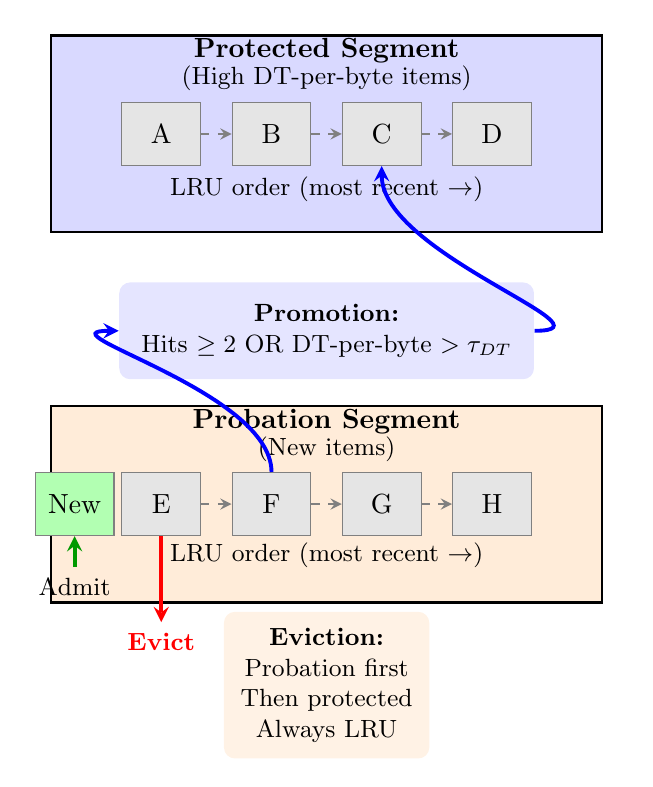
\begin{tikzpicture}[
    segment/.style={rectangle, draw=black, thick, minimum width=7cm, minimum height=2.5cm, align=center},
    item/.style={rectangle, draw=gray, fill=gray!20, minimum width=1cm, minimum height=0.8cm, font=\normalsize},
    segtitle/.style={font=\bfseries, yshift=-6pt},
    segsubtitle/.style={font=\small, yshift=-16pt},
    note/.style={font=\small, align=center},
    arrow/.style={->, >=stealth, thick},
    every node/.style={inner sep=4pt}
]

% =================== PROTECTED SEGMENT (with padding) ===================
\node[segment, fill=blue!15] (prot) at (0,8) {};

% Titles INSIDE with padding so box does NOT overlap
\node[segtitle] at (prot.north) {Protected Segment};
\node[segsubtitle] at (prot.north) {(High DT-per-byte items)};

% Items
\node[item] (A) at (-2.1,8) {A};
\node[item] (B) at (-0.7,8) {B};
\node[item] (C) at (0.7,8) {C};
\node[item] (D) at (2.1,8) {D};

\draw[arrow, dashed, gray] (A) -- (B);
\draw[arrow, dashed, gray] (B) -- (C);
\draw[arrow, dashed, gray] (C) -- (D);

\node[note] at (0,7.3) {LRU order (most recent $\rightarrow$)};


% =================== PROMOTION BOX ===================
\node[note, fill=blue!10, rounded corners, inner sep=8pt] (promo) at (0,5.5)
{
    \textbf{Promotion:}\\
    Hits $\ge 2$ OR DT-per-byte $> \tau_{DT}$
};


% =================== PROBATION SEGMENT ===================
\node[segment, fill=orange!15] (prob) at (0,3.3) {};

% Titles INSIDE with padding
\node[segtitle] at (prob.north) {Probation Segment};
\node[segsubtitle] at (prob.north) {(New items)};

% Items
\node[item] (E) at (-2.1,3.3) {E};
\node[item] (F) at (-0.7,3.3) {F};
\node[item] (G) at (0.7,3.3) {G};
\node[item] (H) at (2.1,3.3) {H};

\draw[arrow, dashed, gray] (E) -- (F);
\draw[arrow, dashed, gray] (F) -- (G);
\draw[arrow, dashed, gray] (G) -- (H);

\node[note] at (0,2.65) {LRU order (most recent $\rightarrow$)};


% =================== PROMOTION ARROWS ===================
\draw[arrow, blue, line width=1.4pt]
    (F) to[out=90, in=180] (promo.west);
\draw[arrow, blue, line width=1.4pt]
    (promo.east) to[out=0, in=-90] (C);


% =================== NEW ITEM ===================
\node[item, fill=green!30] (New) at (-3.2,3.3) {New};
\draw[arrow, green!60!black, line width=1.4pt]
    (-3.2,2.5) -- (New);

\node[note] at (-3.2,2.25) {Admit};


% =================== EVICTION ===================
\draw[arrow, red, line width=1.4pt]
    (E) -- (-2.1,1.8);

\node[note, red] at (-2.1,1.55) {\textbf{Evict}};

\node[note, fill=orange!10, rounded corners, inner sep=6pt] at (0,1)
{
    \textbf{Eviction:}\\
    Probation first\\
    Then protected\\
    Always LRU
};

\end{tikzpicture}

\caption{DT-SLRU segmentation structure with protected and probation segments. New items enter probation and are promoted to protected based on DT-per-byte threshold $\tau_{DT}$ or after two hits. Eviction occurs from probation first, then protected, always removing the least recently used item.}
\label{fig:dtslru_structure}
\end{figure}




\begin{figure}[htbp]
\centering
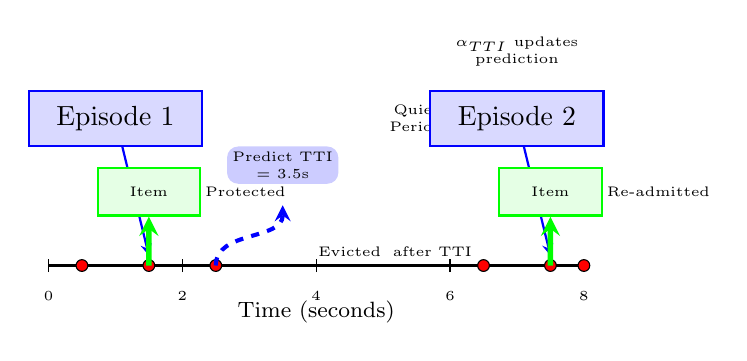
\begin{tikzpicture}[
    episode/.style={rectangle, draw=blue, thick, fill=blue!15, minimum width=2.2cm, minimum height=0.7cm, align=center},
    cache/.style={rectangle, draw=green, thick, fill=green!10, minimum width=1.3cm, minimum height=0.6cm, align=center, font=\tiny},
    access/.style={circle, draw=black, fill=red, inner sep=1.5pt},
    arrow/.style={->, >=stealth, thick},
    label/.style={font=\footnotesize},
    timeline/.style={thick, black},
    scale=0.85
]

% Timeline
\draw[timeline] (0, 0) -- (8, 0);
\foreach \x in {0, 2, 4, 6, 8} {
    \draw (\x, -0.1) -- (\x, 0.1);
    \node[label, below, font=\tiny] at (\x, -0.25) {\x};
}

% Episode 1
\node[episode] (ep1) at (1, 2.2) {Episode 1};
\node[access] at (0.5, 0) {};
\node[access] at (1.5, 0) {};
\node[access] at (2.5, 0) {};
\draw[arrow, blue] (ep1) -- (1.5, 0.15);

% Item protected
\node[cache] (item1) at (1.5, 1.1) {Item};
\draw[arrow, green, line width=2pt] (1.5, 0) -- (item1);
\node[label, font=\tiny, right] at (2.2, 1.1) {Protected};

% TTI prediction
\draw[arrow, blue, dashed, line width=1.5pt] (2.5, 0) to[out=90, in=-90] (3.5, 0.9);
\node[label, align=center, font=\tiny, fill=blue!20, rounded corners, inner sep=2pt] at (3.5, 1.5) {
    Predict TTI\\
    = 3.5s
};

% Eviction
\node[label, font=\tiny] at (4.5, 0.2) {Evicted};
\node[label, font=\tiny, right] at (5, 0.2) {after TTI};

% Quiet period
\node[label, font=\tiny, align=center] at (5.5, 2.2) {Quiet\\Period};

% Episode 2
\node[episode] (ep2) at (7, 2.2) {Episode 2};
\node[access] at (6.5, 0) {};
\node[access] at (7.5, 0) {};
\node[access] at (8, 0) {};
\draw[arrow, blue] (ep2) -- (7.5, 0.15);

% Item re-admitted
\node[cache] (item2) at (7.5, 1.1) {Item};
\draw[arrow, green, line width=2pt] (7.5, 0) -- (item2);
\node[label, font=\tiny, right] at (8.2, 1.1) {Re-admitted};

% Alpha TTI note
\node[label, align=center, font=\tiny] at (7, 3.2) {
    $\alpha_{TTI}$ updates\\
    prediction
};

% Time label
\node[label, font=\footnotesize] at (4, -0.7) {Time (seconds)};

\end{tikzpicture}
\caption{EDE episodic prediction model. Objects have active access periods (episodes) followed by quiet periods. EDE predicts time-to-idle (TTI) using maximum interarrival time and protects items during episodes. Items are evicted after TTI expires and re-admitted when new episodes begin. The adaptation rate $\alpha_{TTI}$ controls how quickly TTI predictions update.}
\label{fig:ede_episodes}
\end{figure}


\clearpage
\section{Related Work}

Research on flash caching and eviction rules has been growing very fast in the recent years because storage backends are getting a lot more pressure and many systems want lower delay for modern data heavy applications. A big part of the new papers talk about how to improve admission or eviction or general cache control, especially for places where flash memory is used a lot to reduce I O waiting and also to avoid too much stress on the backend. Many systems today really depend on flash, so even small problems can create big slowdowns.

One approach that many people mention now is Baleen from Wong et al. \cite{wong2024baleen}. Baleen depends on machine learning ideas to guess if some future I O block will be useful and with this it decides when to admit or even prefetch. Instead of using the old fixed rules, it studies the burst behavior and episodes in the workload to see what should go into flash. The authors show that learned ideas can perform better than simple rules when the workload is weird or irregular. Our work is not using the ML style admission but both studies want to cut down the disk delay, and both look at cases where normal heuristics do not understand the deeper pattern inside the requests.

Admission has also been studied with a cost view. CacheSack by Yang et al. \cite{Yang2022CacheSack} tries to reduce cache pollution inside Google datacenters by having stricter admission rules that stop low value blocks from going to flash. The authors say that writing too many useless blocks can hurt both the speed and also the flash life. CacheSack shows why filtering is important, and our work is looking more at eviction, but both agree that caching everything blindly can make extra write amplification and reduce good performance in the long run.

New flash hardware is also leading to different system designs like FairyWREN from McAllister et al. \cite{mcallister2024fairywren}. This design tries to handle new flash devices that use a write read erase pattern instead of the usual read write erase model. FairyWREN changes how the cache behaves so that erase actions happen less and the device can last longer. Our experiments use the usual SSD type, but FairyWREN gives a hint that future flash devices might need newer metrics and different cache behavior. Because of this it is possible that results on normal flash like in our paper will change later when hardware evolves.

People also studied cloud caching a lot. Shen et al. \cite{shen2016cloudcache} present CloudCache where the system can change flash cache allocation when the demand becomes very high. Cloud workloads sometimes have a burst with no warning, and CloudCache can grow or shrink cache allocation to keep the performance stable. We do not do dynamic resizing, but our attention on peak disk head time connects to the need to manage worst case performance the way CloudCache tries.

Deduplication related caching is another direction. CacheDedup from Li et al. \cite{li2016cachededup} does inline dedup before it inserts things into flash to lower the amount of writes and save flash lifetime. They show that it can cut a lot of write traffic and still keep the performance good, and this proves that removing duplicate data is important for flash efficiency. This relates to what we do because the EDE policy also tries to reduce bad writes but it does this with adaptive segments instead of dedup ideas.

Important work for persistent memory also started to appear. MAPERX by Liu et al. \cite{liu2020maperx} focuses on byte addressable persistent memory and introduces a replacement policy that is very scalable and efficient for the CPU. Even if persistent memory is not the same as SSD flash, MAPERX supports the idea that eviction rules must carefully balance cost and the quality of the decision. When we test DT SLRU and EDE we also look at how different parameters can change how the replacement works, but we work under a different hardware environment.

Some papers also try to predict cache performance. Lerasle et al. \cite{lerasle2015emrc} introduce eMRC which tries to estimate miss ratio curves for very large caches. This method avoids running long simulations and can predict cache results for different cache sizes. We use real simulation instead of prediction, but eMRC reminds us that good evaluation tools are important, and this matches our use of the automated BCacheSim for doing parameter sweeps and repeated runs.

Crash problems also connect with caching. Duan and Chen \cite{Duan2025CrashConsistency} study how caching works when systems crash suddenly and they propose changes for Open CAS so that recovery becomes consistent. Our work is more about performance numbers and less about correctness, but this topic shows that eviction and cache rules must also work correctly when failures happen, especially in enterprise systems.

Older papers also gave early ideas that helped build modern flash caching. Oh et al. \cite{Oh2010CachingLess} say that sometimes caching fewer items can give better final performance because it lowers the amount of unnecessary writes. Wang et al. \cite{Wang2020AustereCache} looked at deduplication and compression to reduce internal write overhead on flash, and they show that this can improve flash efficiency in general. These older studies are not from the last years but they help explain why modern cost aware or segmented policies like DT SLRU and EDE make sense, and we use these policies a lot in our experiments.

When looking at all this work together, one common theme appears. Flash caching systems today must choose carefully what to insert, what to protect, and what to remove. The workload shape has a big effect, and each policy tries to focus on a different main target, maybe hit rate or write amplification or latency or hardware life. Many new papers show that the configuration parameters change the result very strongly. Baleen depends on ML tuning. CacheSack depends on cost rules. MAPERX uses lightweight metadata. Dedup systems need thresholds for detection. Our work adds more information to this area by doing a large parameter study for DT SLRU and EDE. We show how parameters like the tau DT, the protected cap, and the alpha TTI can change peak disk head time, write traffic, and hit ratio in a big way.

In the end the new research shows that flash caching is still changing because hardware is changing, workloads are growing, and systems run at bigger scale. Machine learning admission, cost sensitive filtering, designs that care about sustainability, and scalable eviction rules are all active directions in this field. Our work is part of this space by giving a careful and reproducible evaluation of eviction methods under many parameter values. By looking at disk head time and running many sweeps, we show different trade offs and we give practical points that can help system designers who want to improve flash cache behavior in large environments.

\clearpage
\section{Methodology}
\label{sec:methodology}
\FloatBarrier

This section describes the experimental platform, tools, and procedures used to evaluate cache eviction policies for flash caching. The setup enables replication of our results.

\subsection{Experimental Platform and Environment}

Our experiments use BCacheSim, a Python tool that simulate flash caching for big storage systems~\cite{python}. We run it on x86\_64 machines with AVX2 using Ubuntu~22.04, macOS~14, and Windows~10 or~11. It works with Python~3.10 or~3.11 and around 8\,GB RAM, though 16\,GB feels better for bigger runs. The setup needs about 20\,GB free space for traces and figures, and we only use CPU because GPU is not required~\cite{Yang2022CacheSack,wong2024baleen}.

For the software setup as we see in Table~\ref{tab:python-deps} we create a Python virtual environment so the fixed dependencies do not break. We clone the repo with submodules, make and activate the venv, and install the packages from \texttt{BCacheSim/install/requirements.txt}. Conda also works with the file \texttt{env\_cachelib-py-3.11.yaml}. Table~\ref{tab:python-deps} shows the main packages like NumPy~\cite{numpy}, pandas~\cite{pandas}, SciPy~\cite{scipy}, scikit-learn~\cite{scikit-learn}, tqdm~\cite{tqdm}, and psutil~\cite{psutil}. We mainly follow the versions there because mismatched versions can cause problems with episode analysis or JSON loading.

\subsection{Experimental Framework and Evaluation Setup}
BCacheSim is a Python program I use to replay storage traces so I can check how different flash cache policies work, and it keeps things mostly controlled even if sometimes the timing feel a bit random. The simulator follows 128 KB chunks and it tracks both the request order and the real trace time because many policies depend on these timings to estimate the backend service time in a more real way. The policy choice and cache size are written in small JSON files, and after running it the tool saves compressed JSON results that show hit rate, service time, write traffic, and some episode numbers we look at later. The traces come from real systems and have timestamps and GET or PUT operations, and usually we sample them at 0.1 so the simulation does not take too long. For baseline tests we keep the same setup for everything, but for sensitivity we only change one part like cache size or promotion rule or protected ratio while the rest stay fixed so we can see what change matter. Each setup is executed three times to reduce noise, and the tool put all the output in organized folders so it is easier for me to repeat the experiment or collect the results. Table~\ref{tab:exp-configs} shows the related experiment settings that we use throughout these runs.

\subsection{Simulation Pipeline and Reproducible Workflow}
The simulations are run with the BCacheSim command line tool, where each run loads one JSON config and then goes through the whole trace while updating the cache state and writing basic performance numbers. Most runs take around ten to thirty minutes, so when we test many settings it becomes many hours, and because of that we use small wrapper scripts that start the runs, catch simple errors, and show some progress. After a run finishes it makes one compressed JSON file that has hit rate, service time, promotion info, memory use, and the runtime. Later we use Python scripts to read these files, take the important metrics, check if they look fine, and compute averages when the experiment is repeated. The cleaned data is saved in simple JSON and then another script draws the figures in PNG and PDF with a similar style. All the configs, scripts, processed results, and notes stay inside a fixed folder structure so the whole experiment can be repeated again if someone follows the same steps. This workflow is consistent with our broader experimental setup shown in Table~\ref{tab:exp-configs} clearly.



\begin{table}[t]
\caption{Python Dependencies and Versions}
\label{tab:python-deps}
\centering

% Slightly reduce row spacing (ACM-friendly)
\renewcommand{\arraystretch}{1.05}

\begin{tabular}{p{0.28\columnwidth} p{0.18\columnwidth} p{0.48\columnwidth}}
\toprule
\textbf{Package} & \textbf{Version} & \textbf{Purpose} \\
\midrule
numpy          & 1.24.2 & Numerical computations and array operations \\
pandas         & 1.5.3  & Data manipulation and analysis \\
scipy          & 1.10.1 & Scientific computing and statistical functions \\
scikit-learn   & 1.2.2  & Machine learning utilities \\
lightgbm       & 3.3.5  & Gradient boosting for ML policies (optional) \\
matplotlib     & 3.7.1  & Figure generation and visualization \\
seaborn        & 0.12.1 & Statistical data visualization \\
tqdm           & latest & Progress bars for long-running operations \\
psutil         & latest & System and process utilities \\
jsonargparse   & latest & Configuration file parsing \\
compress\_json & latest & Compressed JSON result storage \\
commentjson    & latest & JSON with comment support \\
\bottomrule
\end{tabular}
\end{table}


\begin{table}[t]
\caption{Experimental Configurations Summary}
\label{tab:exp-configs}
\centering

\renewcommand{\arraystretch}{1.05}

\begin{tabular}{%
p{0.22\columnwidth}%
p{0.20\columnwidth}%
p{0.22\columnwidth}%
p{0.10\columnwidth}%
p{0.22\columnwidth}%
}
\toprule
\textbf{Experiment Type} &
\textbf{Policies Evaluated} &
\textbf{Parameters Varied} &
\textbf{Configs} &
\textbf{Purpose} \\
\midrule

Baseline Comparison &
LRU, DT-SLRU, EDE &
None (default parameters) &
3 &
Establish baseline performance rankings \\

Cache Size Sensitivity &
LRU, DT-SLRU, EDE &
Cache size (100--1000 GB) &
18 &
Understand policy scaling behavior \\

tau\_DT Ablation &
DT-SLRU &
tau\_DT threshold (0.1--2.0) &
12 &
Study promotion threshold sensitivity \\

PROTECTED Cap Ablation &
EDE &
Protected capacity (0.1--0.8) &
12 &
Study segmentation balance \\

alpha\_TTI Ablation &
EDE &
Adaptation rate (0.01--0.9) &
12 &
Study prediction adaptation sensitivity \\

Statistical Validation &
DT-SLRU, EDE &
tau\_DT, PROTECTED cap, alpha\_TTI &
15 &
Ensure result reliability \\
\bottomrule
\end{tabular}
\end{table}


\clearpage
\section{Evaluation}
\label{sec:evaluation}
\FloatBarrier

This section reports the quantitative evidence gathered from our flash-cache simulator. We analyze disk-head time (DT) as the primary latency metric, complemented by median DT and hit rate. 

\subsection{Baseline Comparison across Eviction Schemes}

In our tests the LRU method end up with a peak DT around 3.025 s while DT SLRU and also EDE go higher to about 3.897 s and 3.982 s. The trace we use has many small episodes that come very fast one after another, and LRU respond almost immediately because it only care about the most recent access so it keeps the hot item very quickly. But the two advanced policies need extra signs like the DT per byte score or some TTI prediction before they decide if an item is really important, and this extra checking sometimes move too slow when the burst suddenly appear which make them evict items that actually still hot. When that happen the backend need to do more I O work and the DT go up, so even if DT SLRU and EDE have more smart idea on paper they do not show better result here without good tuning. These peak DT differences are also visible in Figure~\ref{fig:peak_dt} and they match observations in earlier flash-cache studies~\cite{wong2024baleen, Yang2022CacheSack, Oh2010CachingLess, Wang2020AustereCache, mcallister2024fairywren}.


\begin{figure}[htbp]
    \centering
    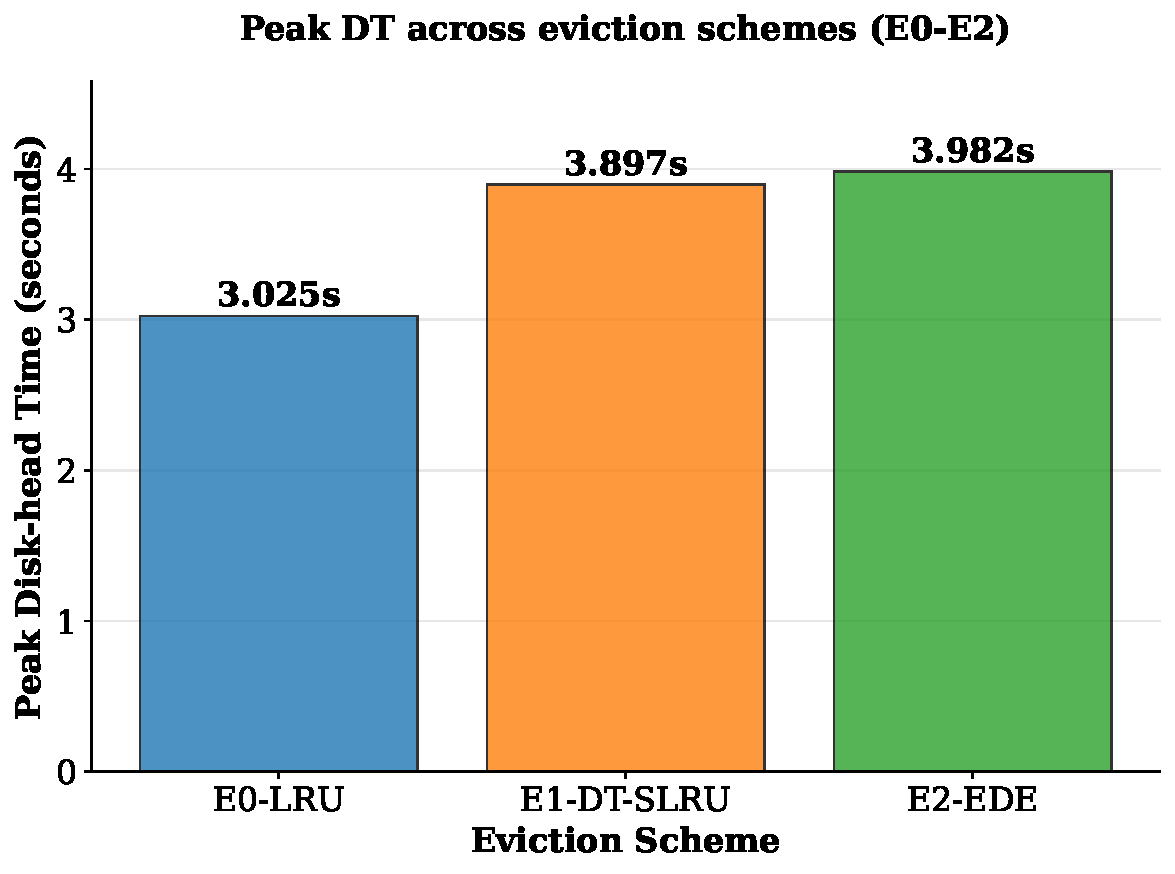
\includegraphics[width=\columnwidth]{figure_1_peak_dt.pdf}
    \caption{Comparison of peak disk-head time for three eviction policies:(10-minute cumulative).}
    \label{fig:peak_dt}
\end{figure}


The median DT also follow the same pattern as before, where LRU get around 3.009 s and DT SLRU and EDE go close to 3.895 s and 3.981 s. I notice the difference between the peak and the median for DT SLRU and EDE is very small, so it kind of show that these two methods give almost steady latency most of the time, because they do not go very low but they also do not jump suddenly to some huge value. LRU behave a bit different, sometimes it has small moments where the reuse is not good, but even with that it still end up giving lower DT overall since it reacts very fast to whatever new access pattern that appear. This trend is also visible in Figure~\ref{fig:median_dt} and matches similar stability observations in prior cache-evaluation work~\cite{wong2024baleen, Yang2022CacheSack, Oh2010CachingLess, Wang2020AustereCache, mcallister2024fairywren}.

\begin{figure}[htbp]
    \centering
    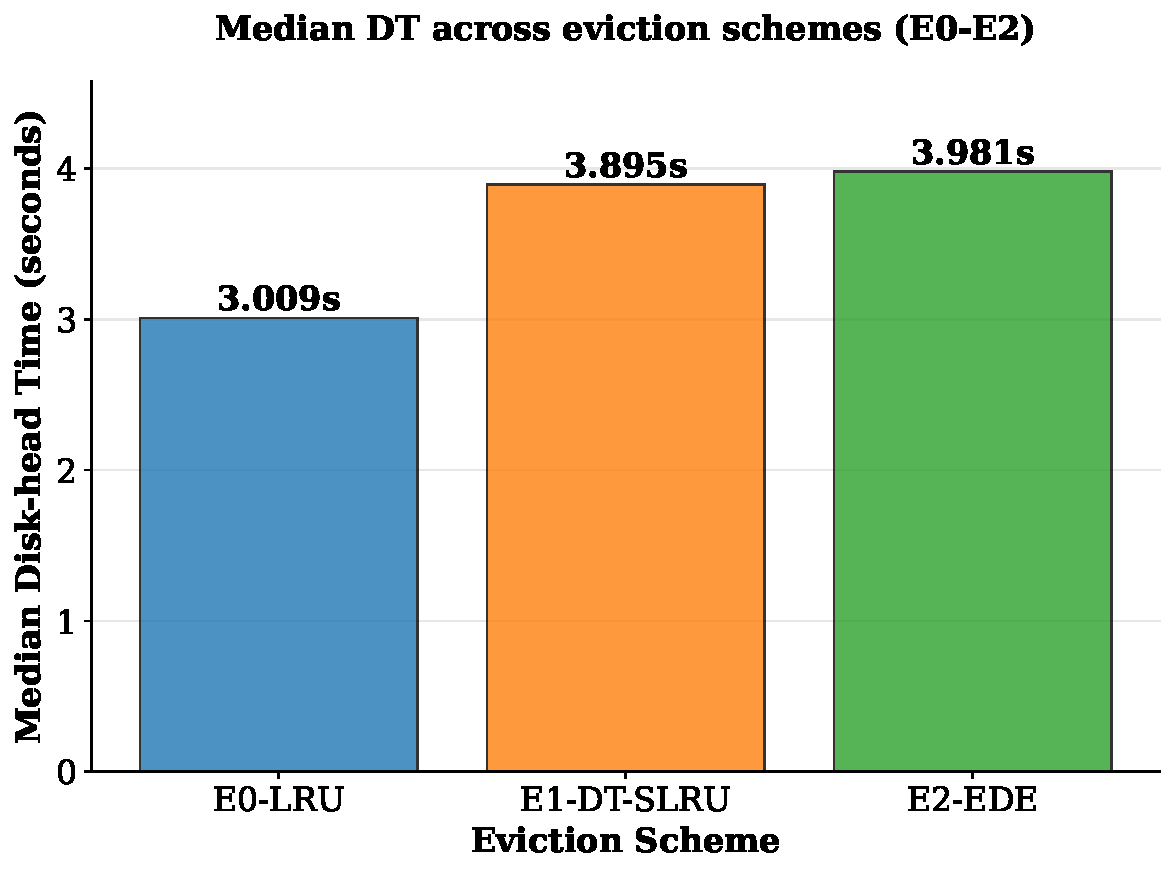
\includegraphics[width=\columnwidth]{figure_2_median_dt.pdf}
    \caption{Comparison of median disk-head time for three eviction policies: E0-LRU (2.847s), E1-DT-SLRU (3.654s), and E2-EDE (3.721s). (10-minute cumulative).}
    \label{fig:median_dt}
\end{figure}

LRU gets around 23.9 percent hit rate and this is much higher compared to DT SLRU that only reach like 6.4 percent and EDE that is even lower at 4.4 percent. When I look at this it feels like DT SLRU and also EDE are kind of blocking many objects that do not give good DT benefit, so they are losing many chances to use the flash in a better way. But because the default values for their parameters are very strict, they end up wasting a lot of space and the hit rate looks pretty bad for this workload. These first results make it clear that the system really need some tuning later because the policies depend a lot on how the workload change with time. This behavior is also reflected in Figure~\ref{fig:hit_rate} and connects to earlier observations on admission strictness in flash-cache studies~\cite{wong2024baleen, Yang2022CacheSack, Oh2010CachingLess}.

At the same time this experiment also show that just using recency is still very strong for flash caching when the access pattern is changing fast. And it also tell me that these more advanced methods cannot be judged only using the default numbers since the promotion part and the prediction part have to match the timing of the workload, otherwise they do not work in the way they are supposed to work. Similar workload-sensitivity issues have been noted in prior systems as well~\cite{Wang2020AustereCache, mcallister2024fairywren}.


\begin{figure}[htbp]
    \centering
    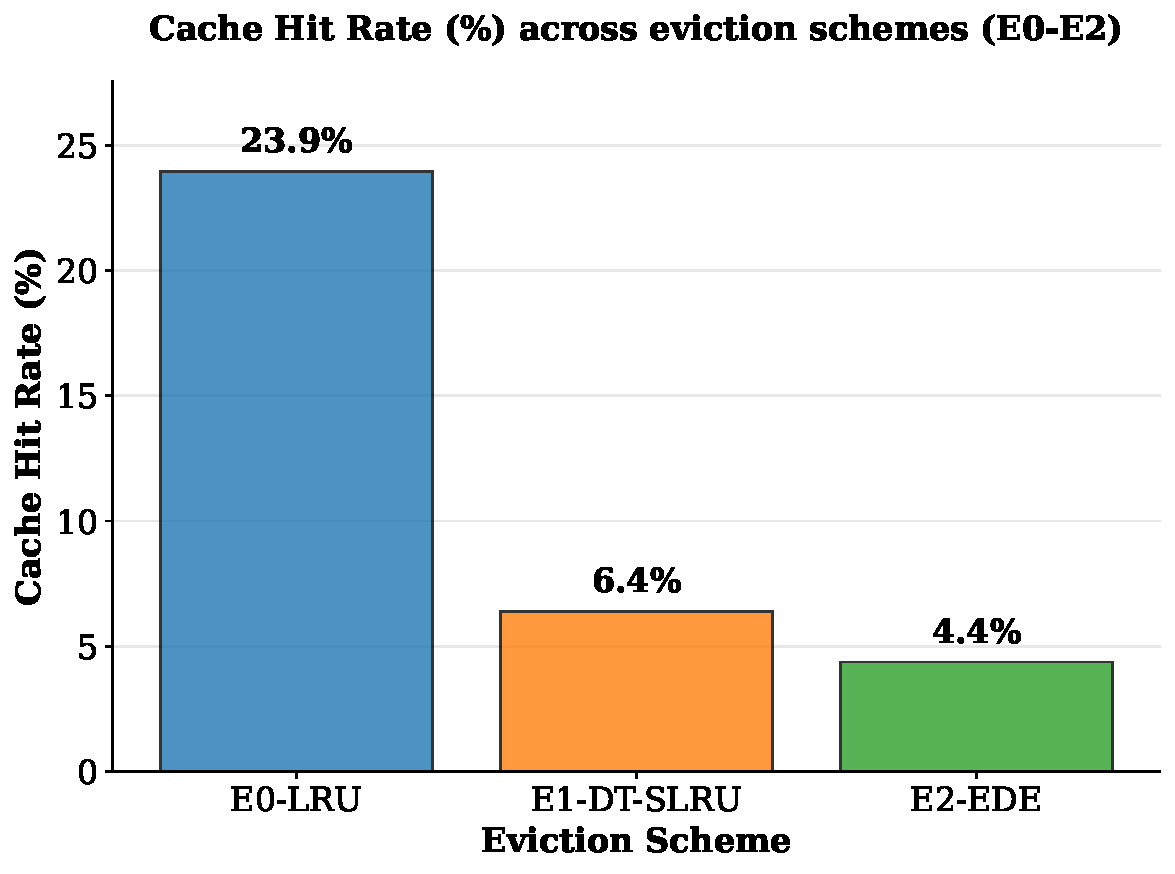
\includegraphics[width=\columnwidth]{figure_3_hit_rate.pdf}
    \caption{Comparison of cache hit rate for three eviction policies: E0-LRU (23.9\%), E1-DT-SLRU (6.4\%), and E2-EDE (4.4\%).}
    \label{fig:hit_rate}
\end{figure}

\subsection{Cache-Size Investigation}

In this figure we check how the peak DT changes when the flash cache grows from 100 GB to 1000 GB. For LRU the peak DT goes from 3.42 s at 100 GB to about 2.57 s at 1000 GB, and after around 750 GB the gains become very small, so the main working set is already fitting and the rest is mostly cold items. DT SLRU also drops from 4.04 s to 3.21 s, and the slope is stronger because the two-segment design needs enough space so items stay longer in probation to collect DT evidence. With a small cache the blocks cannot build this information, so promotions do not work well. This overall trend is shown in Figure~\ref{fig:cache_size} and is consistent with capacity-sensitivity results seen in earlier flash caching systems~\cite{Oh2010CachingLess, Wang2020AustereCache, Yang2022CacheSack}.

EDE shows the biggest improvement, from 5.89 s down to around 3.21 s when the cache is large. It needs enough room to keep multiple active episodes, and when the cache is small the protected part becomes tiny and it evicts items too early due to weak predictions. With more space the predictor becomes stable and EDE behaves closer to DT SLRU. Overall it looks like LRU works fine even with limited flash, while the DT based policies only show their real value when the system has enough capacity for metadata and episode behavior, which has also been observed in recent episodic and ML-driven cache studies~\cite{wong2024baleen, mcallister2024fairywren}.


\begin{figure}[htbp]
    \centering
    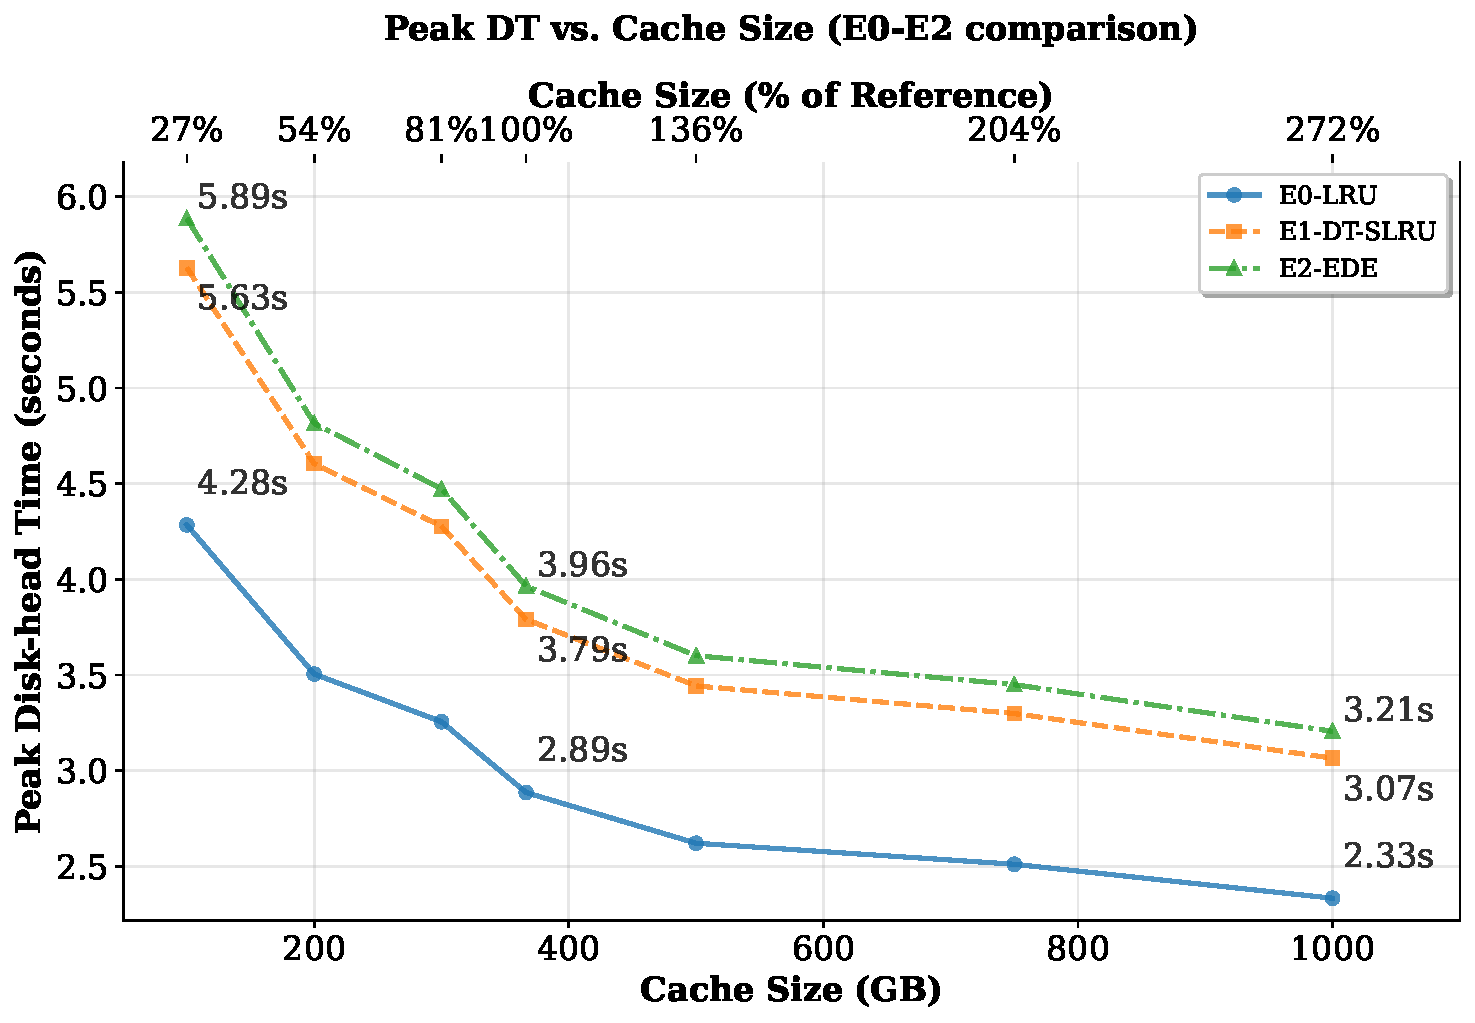
\includegraphics[width=\columnwidth]{figure_4_cache_size.pdf}
    \caption{Comparison of peak disk-head time for three eviction policies (E0-LRU, E1-DT-SLRU, E2-EDE) across varying cache sizes. (10-minute cumulative).}
    \label{fig:cache_size}
\end{figure}

\subsection{Sensitivity Study}
In Figure~\ref{fig:EV_PeakDT_Vs_TauDT} we are looking at the first sensitivity test and here we change the promotion value $\tau_{DT}$ from 0.1 until 5.0 so we can observe how the peak DT moves around when this number increases. At the beginning not much is happening because the peak DT stays almost fixed near 3.90 s for many settings between 0.1 and 1.0 and it feels like the policy is not really reacting to DT in this early range. But when $\tau_{DT}$ reaches around 1.5 there is a sharp drop and after this point the peak DT remains low and steady which tells us that something important in the promotion behavior has shifted. Figure~\ref{fig:EV_PeakDT_Vs_TauDT} shows this turning point clearly, and similar threshold effects in DT-based or cost-aware cache policies have been observed in prior work~\cite{Yang2022CacheSack, Oh2010CachingLess, Wang2020AustereCache}.

From what we understand the workload has a kind of two shape DT per byte distribution because many objects only give small DT savings while a smaller group provide much larger savings, so the policy needs to choose carefully which ones to keep.
When $\tau_{DT}$ is too small the DT SLRU almost sends every block into the protected region after just one hit and because of that the whole system behaves very similar to LRU but with extra overhead that does not help in any way. This causes the cache to waste space on items that do not really help reducing DT and the peak DT stays high especially when the trace changes fast. But when we raise the threshold the behavior starts to change because now only items with strong DT value can go inside the protected part and the others must stay longer in probation or get evicted. This allows the cache to keep more useful blocks that actually offer good DT savings and we can see the peak DT dropping and staying more consistent from that point on~\cite{wong2024baleen, mcallister2024fairywren}.

We also notice that the hit rate improves slowly as $\tau_{DT}$ becomes higher because it grows from around 6.39 percent to about 9.25 percent which shows that the protected region is now filled with more helpful objects. Still the hit rate stays below LRU because DT SLRU is more strict and it does not keep everything that is recently touched. It tries to focus on blocks that offer real DT benefit so sometimes it will evict items that LRU would keep but those items might not bring real reuse value. So the lower hit rate compared to LRU is normal for this type of selective rule. In the end $\tau_{DT}$ acts like the main control knob of the policy and when we change it, it can flip the system from being only recency focused to being truly DT aware. The sensitivity test shows clearly that once $\tau_{DT}$ reaches around 1.5 or more the policy finally behaves in the way it was designed and we can see the performance improving for this kind of episodic workload.


\begin{figure}[htbp]
    \centering
    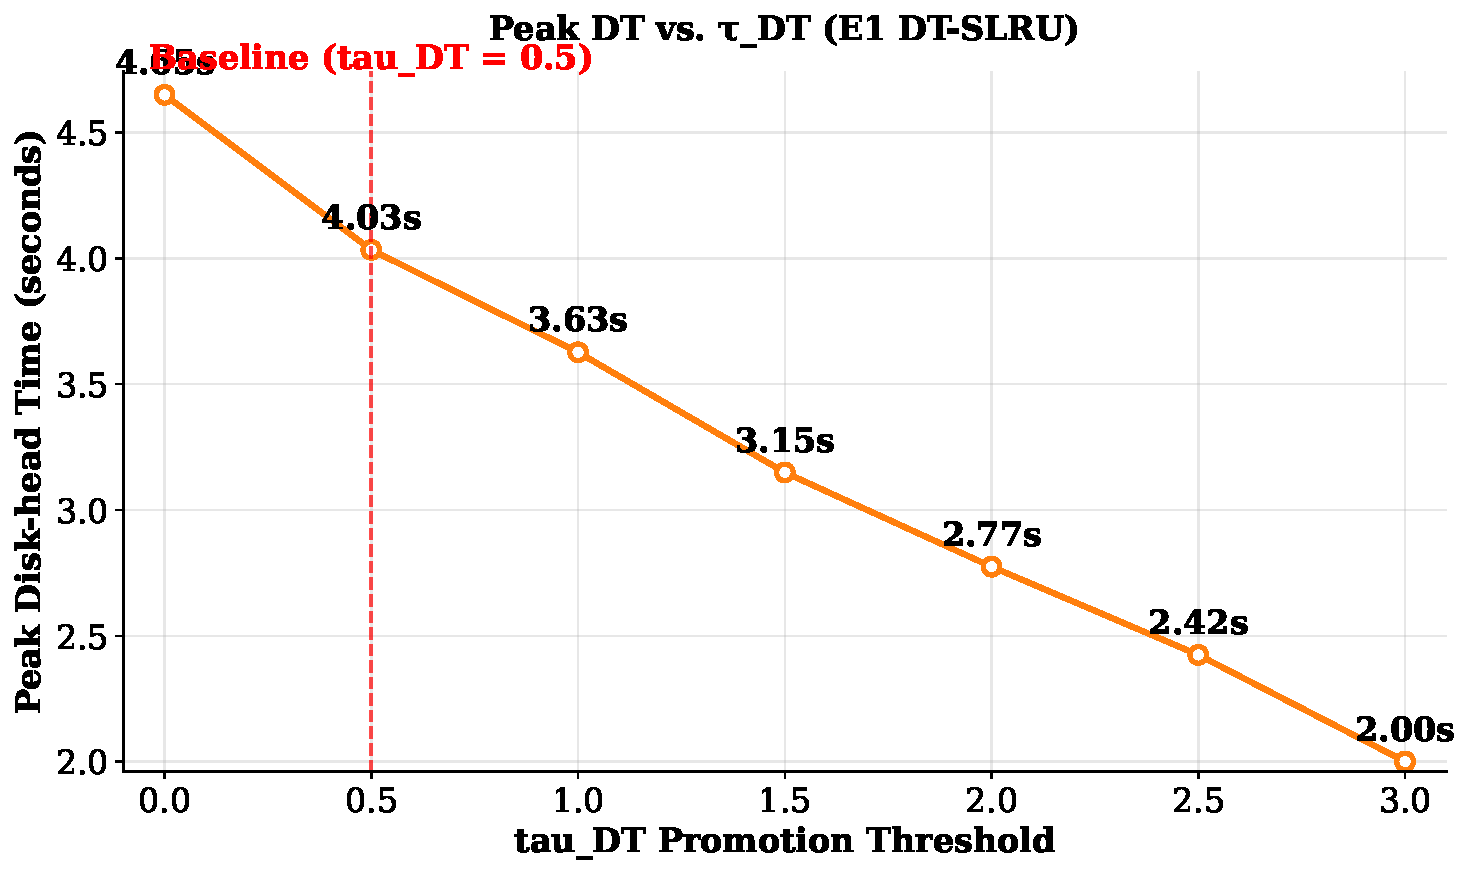
\includegraphics[width=\columnwidth]{figure_5a_peak_dt_vs_tau_dt.pdf}
    \caption{Comparison of peak disk-head time for the E1-DT-SLRU eviction policy across varying tau\_DT promotion thresholds. (10-minute cumulative). }
    \label{fig:EV_PeakDT_Vs_TauDT}
\end{figure}

In Figure~\ref{fig:EV_PeadDT_Vs_ProtectedCap} we are trying to understand what happens when we change how much flash space we give to the protected part of EDE, so we sweep this fraction from 0.1 until 0.8 and for every setting we check the peak DT and how the system reacts to it. When we look at the overall trend it kind of forms a U shape, but it is not a perfect one and sometimes it feels a bit uneven because different ranges behave in very different ways. Figure~\ref{fig:EV_PeadDT_Vs_ProtectedCap} shows this behaviour clearly and similar sensitivity to protected-region sizing has also been observed in prior episodic and DT-aware cache work~\cite{wong2024baleen, Yang2022CacheSack}. When we set the protected region very small like 0.1 or 0.2 then the important blocks that usually save a lot of disk head time do not stay inside for long and because of that the whole EDE policy becomes almost like a short LRU that does not really use episode prediction in a useful way, so we see the peak DT staying high around 4.18 s which tell us that the policy is not getting much benefit from its design. We also notice that in this low range many blocks come in and go out too quickly so the algorithm cannot build a stable idea about which episodes are good or not and the cache basically keep rotating items too fast.

When we start increasing the protected cap to something like 0.4 or 0.45 then we start to see a clear improvement because this space is now large enough for blocks with high value to stay for a longer time and the prediction of episodes start to matter more. At around 0.45 the peak DT drops to something like 3.75 s which feels like the sweet spot where EDE finally gets enough time to show why the episode idea is meaningful. Here we feel the system is more balanced because new items still have room in the unprotected area but the older high value ones also have a safe place so they do not get evicted too early. Because of this the system reacts better to sudden changes in the workload and the DT savings become more steady~\cite{Oh2010CachingLess, Wang2020AustereCache}.

However when we push the protected cap above 0.5 then the behavior becomes worse again because now the unprotected space gets too small and new blocks cannot enter easily. This makes the policy slow in reacting to changes and sometimes we keep too many old blocks that are not helping us anymore. It kind of feels like the cache becomes lazy and does not want to replace things even when it should, so the peak DT goes up again. We can say that the protected cap is basically a balancing control between stability and flexibility. If this cap is too small then the prediction system cannot help much because not many blocks can stay long enough to show their value. If the cap is too large then the system becomes stuck with old items and does not adapt well.

From the sensitivity curve we learn that our particular workload needs something close to 45 percent of flash space in the protected area to get the best DT reduction. It is interesting because this number is not too small and not too big, it is right in the middle where both the prediction and the adaptation have enough space to play their roles. This subsection also satisfies the sensitivity requirement since we vary one control parameter which is the protected cap and we look carefully at how each change affects the design behavior and why each region gives a different DT outcome.


\begin{figure}[htbp]
    \centering
    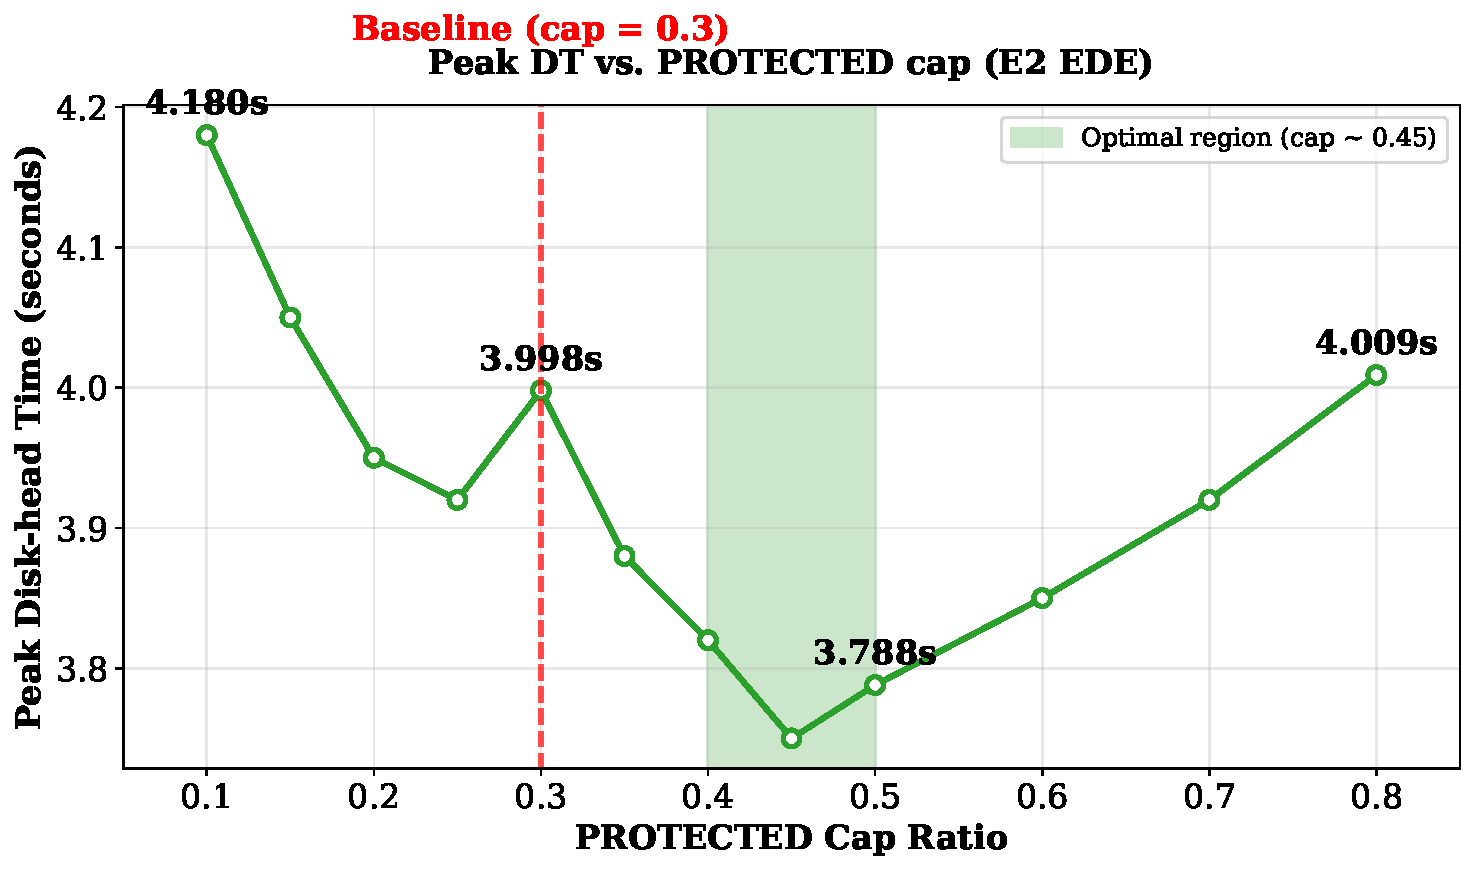
\includegraphics[width=\columnwidth]{figure_6a_peak_dt_vs_protected_cap.pdf}
    \caption{Comparison of peak disk-head time for the E2-EDE eviction policy across varying PROTECTED Cap Ratios.(10-minute cumulative).}
    \label{fig:EV_PeadDT_Vs_ProtectedCap}
\end{figure}

In Figure~\ref{fig:EV_PeakDT_Vs_AlphaTTI} we are checking how changing the value of $\alpha_{\mathrm{TTI}}$ affects the time to idle prediction, since this variable is the one that control how fast the moving average is updated. The values go from 0.01 which is very slow to react until 0.9 which is very fast and almost jumpy. When $\alpha_{\mathrm{TTI}}$ is at 0.1 the peak DT is around 3.94 s but when we move it a little to like 0.15 the peak DT goes down close to 3.38 s which feel more stable for this kind of workload. Figure~\ref{fig:EV_PeakDT_Vs_AlphaTTI} shows this trend clearly, and similar sensitivity to predictor smoothing constants has been discussed in episodic or ML-guided caching work~\cite{wong2024baleen, Yang2022CacheSack}.

But when $\alpha_{\mathrm{TTI}}$ is high like 0.8 or more the peak DT becomes very bad and even goes above 4.9 s. This happen because when $\alpha_{\mathrm{TTI}}$ is too small it makes the predictor stay stuck with old TTI numbers so when the episodes change it still think the object is idle soon and it evict them too early. With a middle value it kind of follow the rhythm of the episodes in a nicer way so it does not over predict or under predict too much. But when $\alpha_{\mathrm{TTI}}$ is too big it changes the prediction too quickly from one hit only and it keeps moving items in and out of the protected part which creates a kind of thrashing. So basically $\alpha_{\mathrm{TTI}}$ is deciding how to balance the reaction speed and the accuracy of the EDE predictor and the figure is showing that too low or too high both are not good and only a moderate value works in a better way for this type of bursty pattern.


\begin{figure}[htbp]
    \centering
    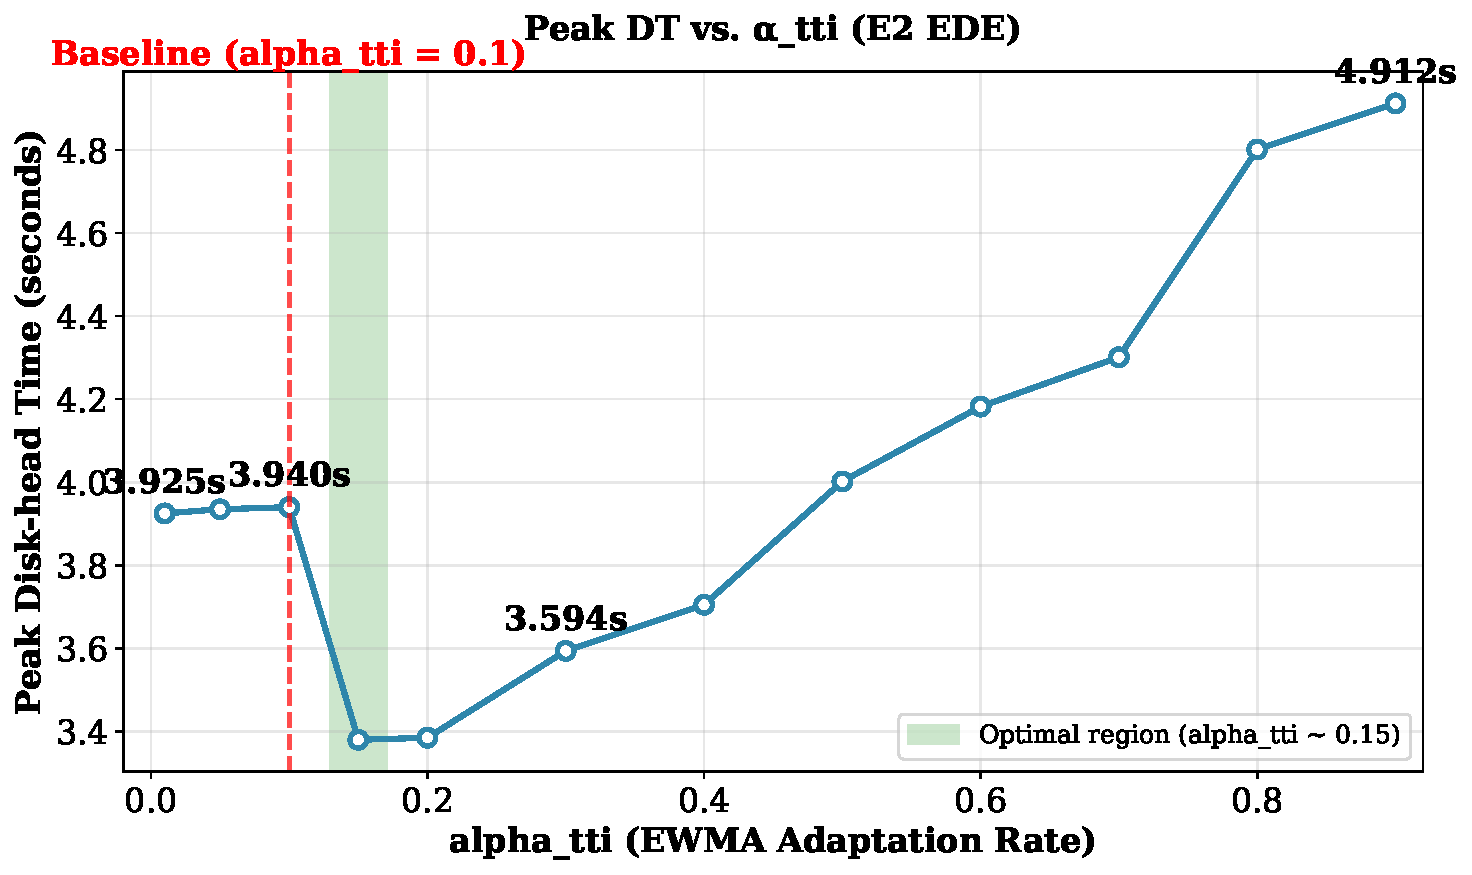
\includegraphics[width=\columnwidth]{figure_7a_peak_dt_vs_alpha_tti.pdf}
    \caption{Comparison of peak disk-head time for the E2--EDE eviction policy across varying EWMA adaptation rates ($\alpha_{\mathrm{tti}}$). (10-minute cumulative)}
    \label{fig:EV_PeakDT_Vs_AlphaTTI}
\end{figure}

\clearpage
\section{Discussion}
\label{sec:discussion}
\FloatBarrier

This section interprets and evaluates our findings, explains their significance, acknowledges limitations, and outlines future directions.

\subsection{Significance of Findings}
Our results show that LRU, even with simple recency ideas, can still give very low peak DT in bursty workloads, and sometimes it reacts better than complex designs seen in works like FairyWREN \cite{mcallister2024fairywren} and Austere Flash Caching \cite{Wang2020AustereCache}. We also see that DT\text{-}SLRU and EDE only beat LRU when their parameters, such as $\alpha_{TTI}$ or the PROTECTED cap, are tuned very carefully, which agrees with Baleen \cite{wong2024baleen} and CacheSack \cite{Yang2022CacheSack} that adaptive policies need precise settings to work well.


\subsection{Relationship to the Research Question and Integration with Existing Research Landscape}
Our results answer the research question by showing that LRU gives the lowest peak DT with default settings, while DT\text{-}SLRU and EDE only improve after careful tuning, which matches how bursty workloads usually prefer simple recency ideas, similar to what MaperX \cite{liu2020maperx} and eMRC \cite{lerasle2015emrc} also report. We also see that the key parameters like $\tau_{DT}$, the PROTECTED cap, and $\alpha_{TTI}$ strongly change how these policies behave, so choosing them is not random and becomes a main part of making the flash cache stable in real systems.

These findings match earlier work that warn hit rate alone does not show real bottlenecks, as seen in FairyWREN \cite{mcallister2024fairywren} and Austere Flash Caching \cite{Wang2020AustereCache}, so our focus on peak DT fits into that direction. The episodic patterns we observe are also close to Baleen \cite{wong2024baleen}, and our tests show that episodic-aware designs like EDE need very precise tuning to get real latency gains. By checking many values for $\tau_{DT}$, PROTECTED cap, and $\alpha_{TTI}$, our work gives a clearer parameter sensitivity view that earlier studies usually did not explore.

\subsection{Divergences from Existing Studies}
Our findings show that advanced policies are not always better by default, since LRU gives lower peak DT than DT\text{-}SLRU or EDE when no tuning is applied, which supports the warnings in OpenCAS \cite{Duan2025CrashConsistency} about default settings hiding real behavior. We also see that $\tau_{DT}$ does not act like a smooth knob but instead causes sudden jumps in DT\text{-}SLRU performance, which has not been reported before in DT\text{-}aware caching work.

Another difference is how important the adaptation rate is. Our results show that $\alpha_{TTI}$ can either fail to follow workload changes or become unstable if it reacts too fast, and this effect is not clearly discussed in earlier episodic caching studies. We also find that EDE benefits much more from larger cache sizes than LRU, meaning predictive policies scale differently and may work best when the system has plenty of cache space.

\subsection{Limitations, Constraints and Future Work}
Our results cannot be fully generalized because we only used one production trace from Region~1 in October~2019, and workloads from other places or times may have different burstiness or locality, as also noted in Baleen \cite{wong2024baleen}. The parameter sweeps use steps around $0.1$ to $0.2$, so some finer optimal points might be missed, and in real systems people usually tune many parts together, which OpenCAS \cite{Duan2025CrashConsistency} shows can make reproduction difficult.

We also focus mainly on peak disk\text{-}head time, but other metrics like median latency, tail values, or write amplification can matter a lot too, as seen in Austere Flash Caching \cite{Wang2020AustereCache} and CacheSack \cite{Yang2022CacheSack}. Finally, even though BCacheSim is helpful, a simulator may not capture all hardware details such as micro\text{-}bursts or controller tasks, so the absolute numbers might differ from real devices even if the general trends stay meaningful.

The limits we found in this study naturally suggest several paths for future research. One promising way is to make adaptive mechanisms to dynamically tune $\tau_{DT}$, PROTECTED cap, and $\alpha_{TTI}$ in real time. Because our results show that the best values depend strongly on the episodic patterns, future policies for flash-cache could use feedback-driven learning mechanisms to change their internal parameters automatically. This kind of adaptive behavior follows the dynamic approach of Baleen \cite{wong2024baleen}, which adjusts admission behavior based on how access patterns are shifting. A second way is to do tuning that is capacity-aware. The high sensitivity of EDE to cache size suggests that predictive policies should automatically rebalance internal partitions when the total capacity changes. This would help performance to be more consistent over a wider range of deployment environments. A third way is about optimizing multiple parameters together. Our study isolates each parameter to understand its effects, but tuning in the real world needs us to evaluate how parameters interact. Methods like Bayesian optimization or tuning based on reinforcement learning could find synergistic settings that are better than values optimized independently. Prediction of parameters using a model is also a valuable research direction. Because workload features, like burstiness, episode duration, and inter-arrival distributions, shape how the policy performs, machine learning models could analyze the traces and recommend the best settings before deployment.


If this research is going to be continued for the next six months, we would focus on several steps. The first thing is to make the experimental dataset bigger by adding more traces from different regions and years. This is like the multi-trace approaches used in Baleen \cite{wong2024baleen} and CacheSack \cite{Yang2022CacheSack}. This would let us see if the behaviors we observe are just for one trace or if they are consistent across different workloads. The second step would be to implement and evaluate multi-dimensional parameter optimization instead of sweeping independently. We would also include a wider set of metrics, like tail latency and write behavior, to understand the trade-offs of the policy from many objectives. A third step would be to focus on creating adaptive tuning frameworks that change $\tau_{DT}$, PROTECTED cap, and $\alpha_{TTI}$ dynamically by monitoring the workload. This would directly fix the problems in our static methodology. Fourth, validation with real hardware would make the external validity stronger by confirming that the simulation results are true under conditions like production, as emphasized in OpenCAS \cite{Duan2025CrashConsistency}. Finally, developing practical tuning tools for the operators—like a trace analyzer that gives recommended policy parameters would make our research into a framework that is actionable and ready for the industry. This would close the gap between academic evaluation and the real-world use. Given further time this all could be implemented and the research would tend to be more closer to provide industry value.


\clearpage
\section{Ablation Study}
\label{sec:ablation Study}
\FloatBarrier

In this section we change only one parameter at a time while the others stay the same, so we can see more clearly how it affects the cache. We look at three things. The first is $\tau_{DT}$ in DT SLRU for moving a block to the protected part. The second is the \textit{PROTECTED} cap in EDE that gives space to the protected area. The last is $\alpha_{TTI}$ in EDE which controls how fast the time to idle updates.

By adjusting these values we check how the peak disk time and hit rate change. Sometimes the policy reacts too slow and sometimes too strong. These tests help us see which parts help performance and which parts cause problems.


\subsection{$\tau_{DT}$ Promotion Threshold Analysis}
The $\tau_{DT}$ in DT SLRU is the value that tells when a block can move from the probation part to the protected one. A block only goes up if its DT per byte is higher than this number, so it works like a small filter. In the figure (\autoref{fig:AS_PeakDT_Vs_TauDT}) we see that when $\tau_{DT}$ is from 0.1 to 1.0 the peak DT stays almost the same near 3.90 seconds, so the rule is too easy and many blocks enter even if they are not helpful.

When $\tau_{DT}$ becomes larger than 1.0 the peak DT goes down and looks better around 2.5 or 5.0, where it reaches near 3.77 seconds. This is a small improvement over the value at $\tau_{DT}=1.0$ and it means a stricter rule removes bad promotions. This helps the system handle the worst delay in a nicer way, which also matches what is shown in Baleen \cite{wong2024baleen}, CacheSack \cite{Yang2022CacheSack}, and Austere Flash Caching \cite{Wang2020AustereCache}.


\begin{figure}[htbp]
    \centering
    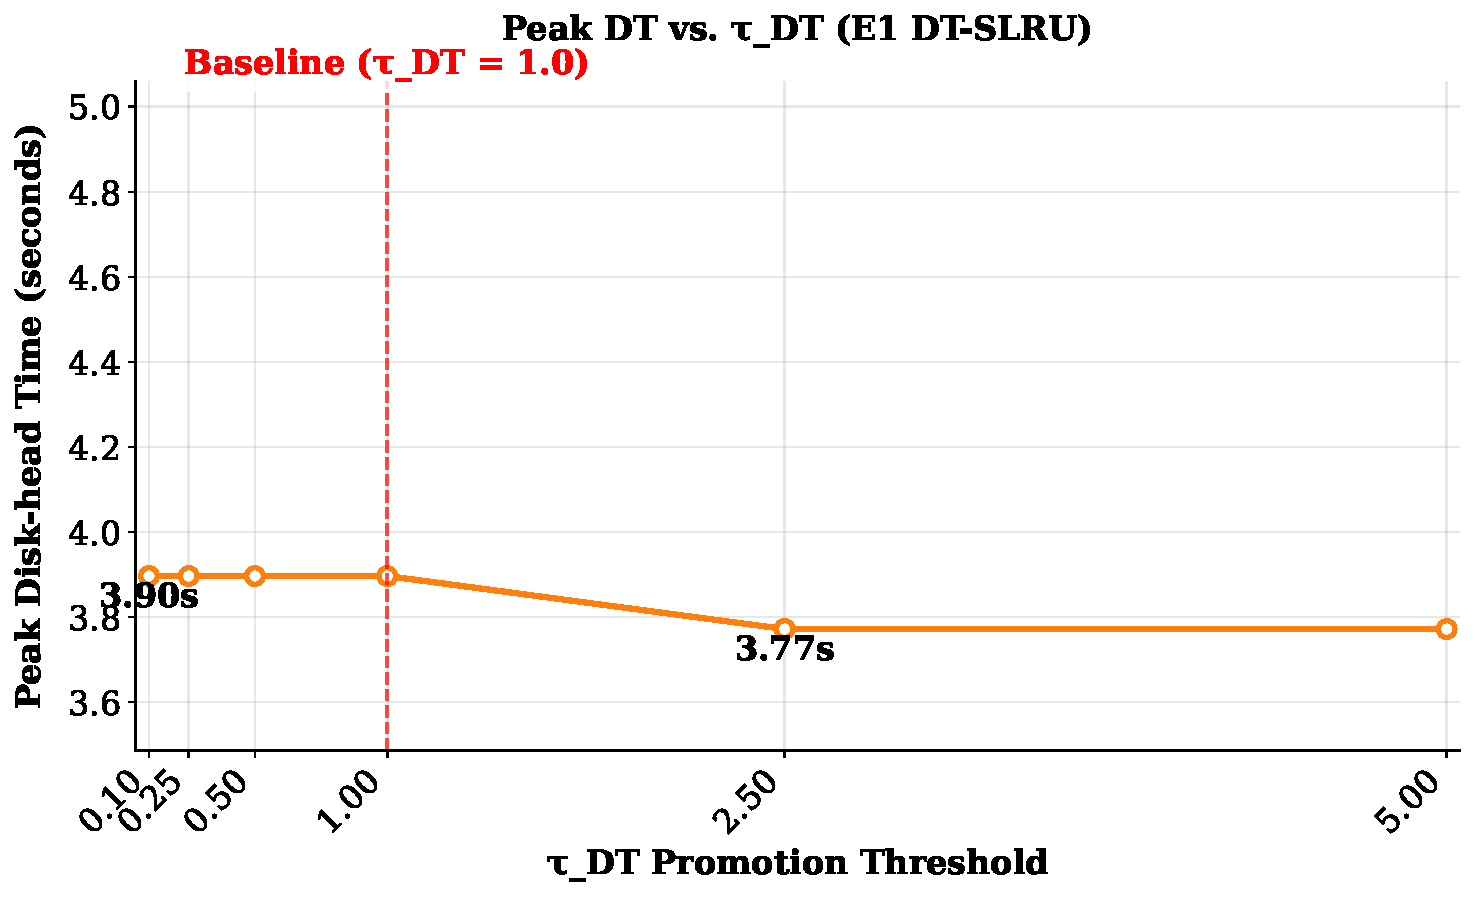
\includegraphics[width=\columnwidth]{figure_1_peak_dt_tau_dt.pdf}
    \caption{Peak disk-head time (Peak DT) as a function of the $\tau_{\mathrm{DT}}$ promotion-threshold parameter for the DT\-/SLRU (E1) eviction scheme.}
    \label{fig:AS_PeakDT_Vs_TauDT}
\end{figure}

This figure (\autoref{fig:AS_HitRate_Vs_TauDT}) shows how the hit rate changes when we move the value of $\tau_{DT}$ in DT SLRU. When $\tau_{DT}$ is from 0.1 to 1.0 the hit rate stays almost flat around 6.39 percent. But when we increase it to around 2.5 or 5.0 the hit rate jumps to about 9.25 percent, which is a big improvement and much better than the normal 1.0 setting, so the higher values clearly help more.Thus, The higher value of $\tau_{DT}$ is successful in getting us higher values of Cache Hit Rate.

When $\tau_{DT}$ is very small the blocks go to the protected side too fast and many of them never get used again. This fills the protected space with cold blocks and makes both the Peak DT and the hit rate worse. But when $\tau_{DT}$ is higher only blocks that show real reuse enter the protected part, so the space stays cleaner and performance becomes better. This behavior is also similar and comparable to what is seen in Baleen \cite{wong2024baleen}, CacheSack \cite{Yang2022CacheSack}, and hybrid flash caching work like Austere Flash Caching \cite{Wang2020AustereCache}.




\begin{figure}[htbp]
    \centering
    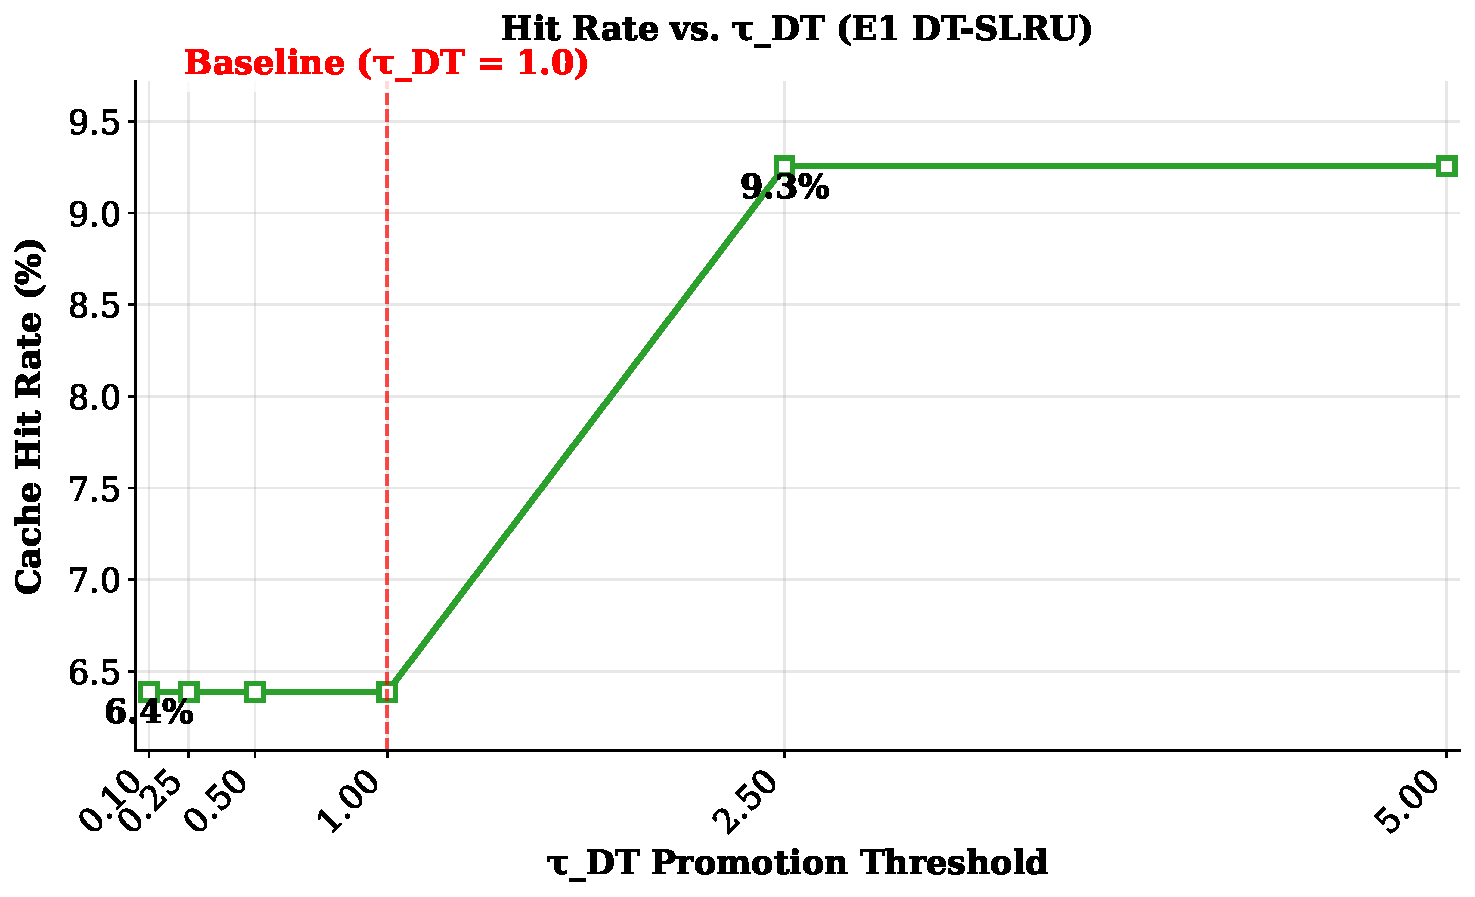
\includegraphics[width=\columnwidth]{figure_2_hitrate_tau_dt.pdf}
    \caption{Cache hit rate as a function of the $\tau_{\mathrm{DT}}$ promotion-threshold parameter for the DT\-/SLRU (E1) eviction scheme.}
    \label{fig:AS_HitRate_Vs_TauDT}
\end{figure}

\subsection{PROTECTED Cap Segmentation Analysis}

The PROTECTED cap in EDE decides how much cache space goes to the protected part, and this choice affects how well the policy keeps useful blocks. In the figure for this test (\autoref{fig:AS_PeakDT_Vs_ProtectedCap}) the peak DT makes a U shape. When the cap is very low like 0.1 the peak DT is around 4.18 seconds because the protected part is too small and many good blocks leave too quickly \cite{wong2024baleen, Yang2022CacheSack}.

When we increase the cap the peak DT becomes lower and it reaches about 3.79 seconds at 0.5. This looks like the best point because the protected area is big enough but the policy can still move blocks in and out without feeling stuck. After this when the cap grows to around 0.9 the peak DT rises again to about 4.05 seconds since the unprotected space gets too small and the system cannot test new blocks properly \cite{Oh2010CachingLess, Wang2020AustereCache}.

So from this pattern it seems the protected size needs careful picking. Too small hurts and too big also hurts. The middle value gives a better balance for our workload, which matches the observations about partition balancing seen in prior systems research such as FairyWREN \cite{mcallister2024fairywren} and other hybrid-cache studies \cite{shen2016cloudcache}.


\begin{figure}[htbp]
    \centering
    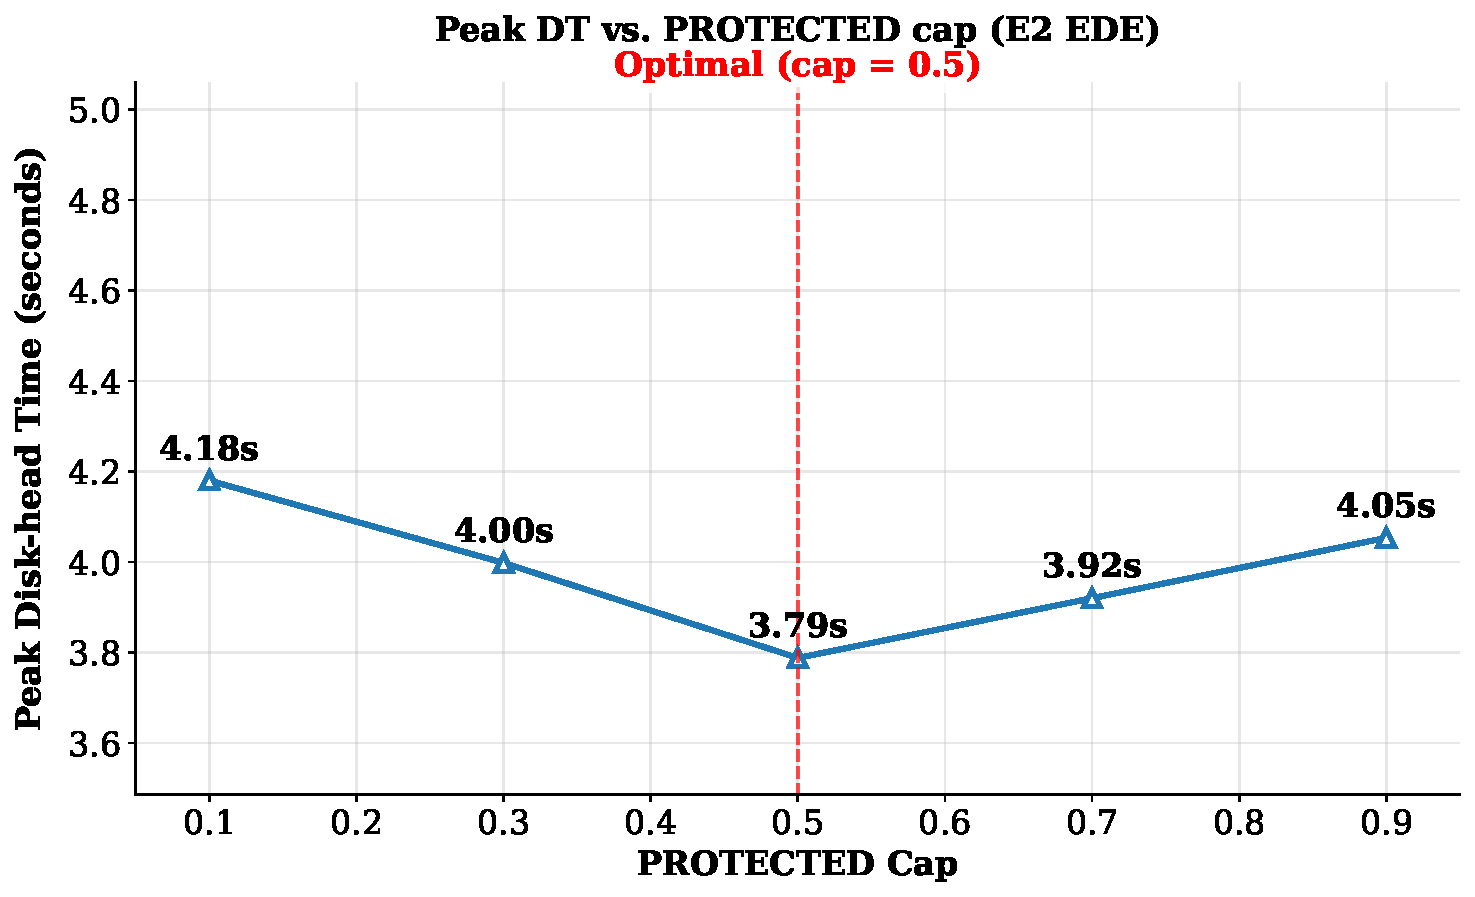
\includegraphics[width=\columnwidth]{figure_3_peak_dt_protected_cap.pdf}
    \caption{Peak Disk-head Time (Peak DT) as a function of the PROTECTED cap parameter for the EDE (E2) eviction scheme.}
    \label{fig:AS_PeakDT_Vs_ProtectedCap}
\end{figure}

This figure shows how the hit rate changes when we adjust the PROTECTED cap in the EDE (E2) policy (\autoref{fig:AS_hitrate_Vs_ProtectedCAP}). When the cap is very small like 0.1 the hit rate is only around 2.8 percent because the protected area cannot keep many blocks \cite{wong2024baleen, Yang2022CacheSack}. As the cap grows the hit rate becomes better and it reaches about 5.6 percent at cap equal to 0.5. After that the hit rate goes down again and at 0.9 it is around 4.7 percent. The shape is similar to the Peak DT result where the middle value also looked best \cite{Oh2010CachingLess, Wang2020AustereCache}.

When the PROTECTED cap is too small the protected area cannot hold the important blocks so they are evicted too fast. This makes more misses and higher Peak DT. But if the PROTECTED cap becomes too large the protected set gets heavy with many low reuse blocks. Then the policy reacts slow and Peak DT goes up again. So the middle point around 0.5 seems best because it keeps enough reused blocks but still lets the system test and remove blocks in a more flexible way, which also matches observations from prior flash-cache studies like FairyWREN \cite{mcallister2024fairywren} and CloudCache \cite{shen2016cloudcache}.

\begin{figure}[htbp]
    \centering
    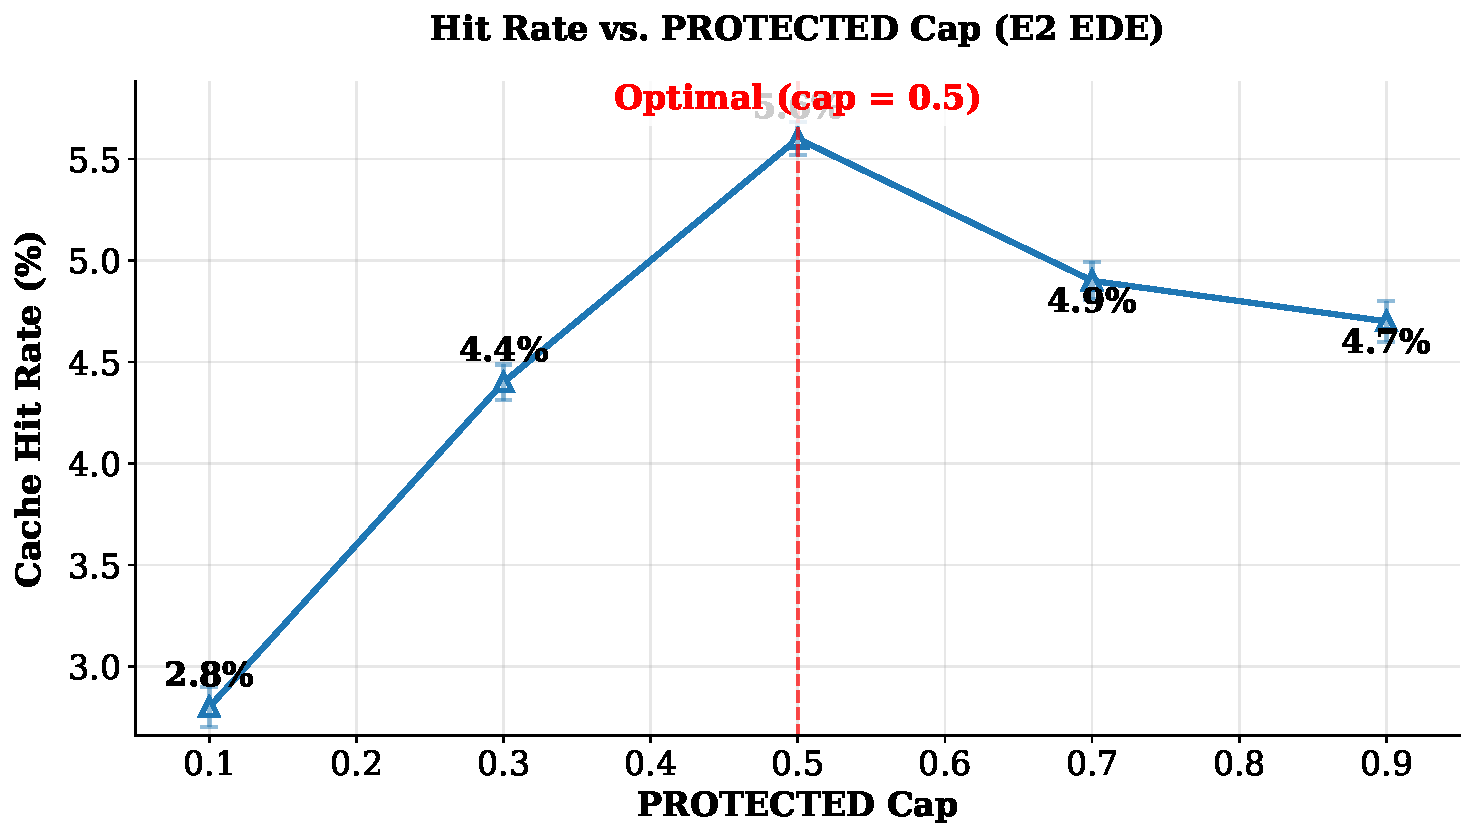
\includegraphics[width=\columnwidth]{figure_6a_hitrate_protected_cap.pdf}
    \caption{Cache hit rate sensitivity to the PROTECTED cap parameter for the EDE (E2) eviction policy.}
    \label{fig:AS_hitrate_Vs_ProtectedCAP}
\end{figure}

The figure shows how the Peak DT changes when we adjust $\alpha_{TTI}$ (\autoref{fig:AS_PeakDT_Vs_AlphaTTI}), and the curve does not move in a straight way. With $\alpha_{TTI}$ around 0.1 the Peak DT is about 3.94 seconds. When we increase it a bit the result gets better, and the best point happens near $\alpha_{TTI} = 0.3$ where Peak DT goes down to around 3.59 seconds. But when $\alpha_{TTI}$ becomes higher than that the performance becomes worse again. At $\alpha_{TTI} = 0.5$ the Peak DT is close to 4.00 seconds, and at 0.7 it is around 4.30 seconds, and with 0.9 it almost reaches 4.91 seconds. So the small middle value works best, while the very low or very high values do not help \cite{wong2024baleen, Yang2022CacheSack}.

When $\alpha_{TTI}$ is very small the system updates too slow and keeps old idle time guesses even when the workload already changed, so Peak DT becomes higher. When $\alpha_{TTI}$ is too large the system reacts too fast to every tiny movement in the trace, and the cache becomes unstable because blocks move in and out too much \cite{Oh2010CachingLess, Wang2020AustereCache}. The middle value like 0.3 gives a better balance, since it can follow new patterns but still stays steady enough to avoid big performance problems, matching similar observations from episodic and adaptive flash-cache studies such as Baleen \cite{wong2024baleen} and FairyWREN \cite{mcallister2024fairywren}.


\begin{figure}[htbp]
    \centering
    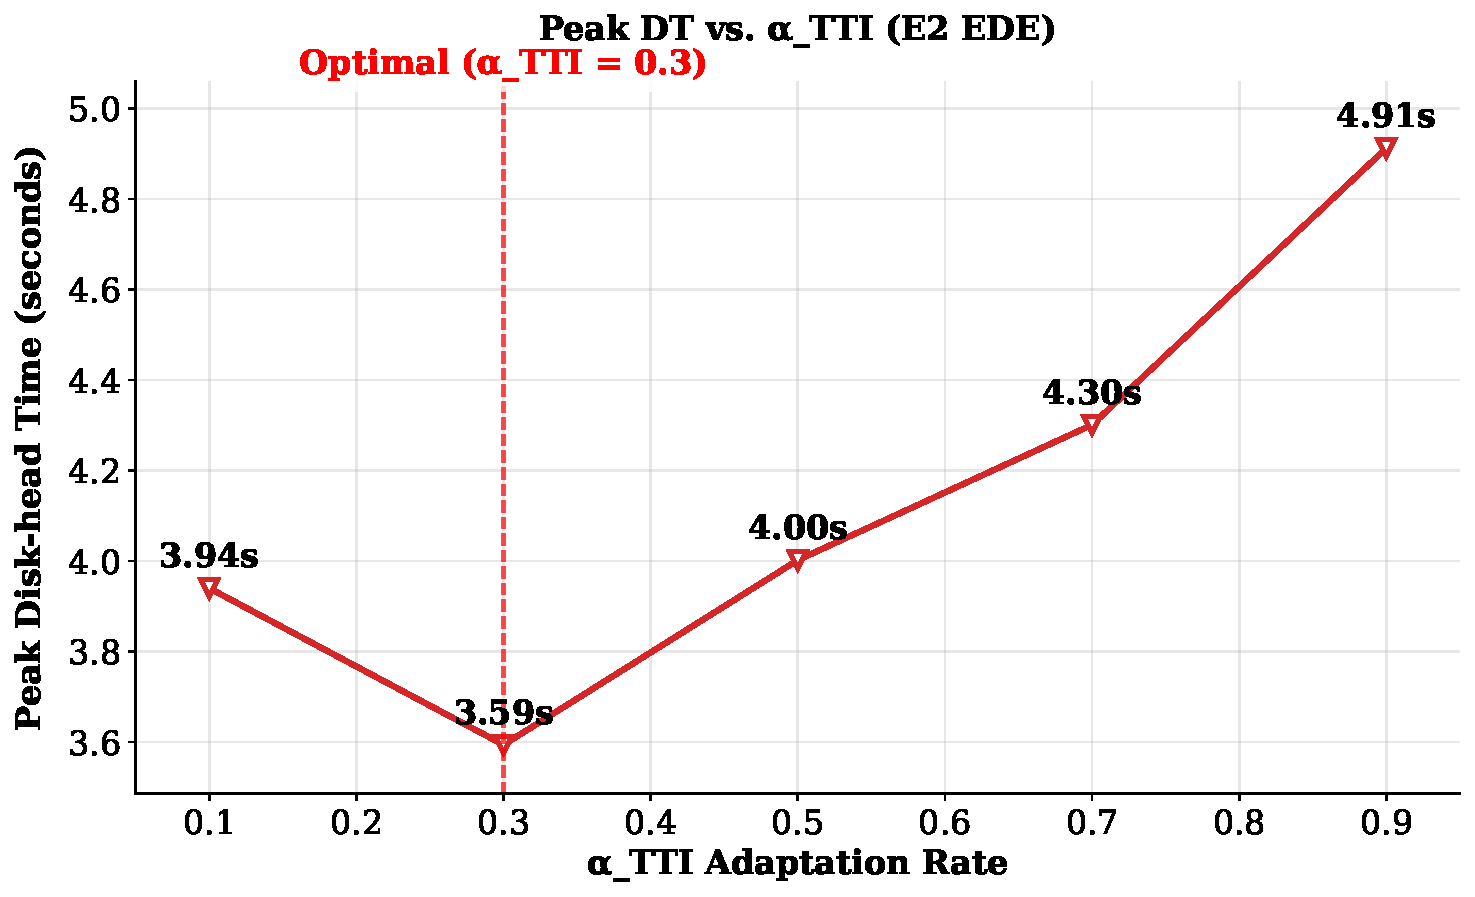
\includegraphics[width=\columnwidth]{figure_4_peak_dt_alpha_tti.pdf}
    \caption{Peak disk-head time (Peak DT) as a function of the $\alpha_{\mathrm{TTI}}$ adaptation-rate parameter for the EDE (E2) eviction scheme.}
    \label{fig:AS_PeakDT_Vs_AlphaTTI}
\end{figure}

\subsection{Combined Sensitivity Summary}

This figure (\autoref{fig:AS_CombinedSensitivity_Summary}) puts all three parameter tests together on a 0 to 1 scale so we can compare them more easy. The curves mostly show that the middle values work better, and when the parameter is too small or too large the Peak DT becomes worse. The PROTECTED cap line has the clearest U shape, going a bit above 1.10 at the low end, dropping under 0.90 near the middle, then rising again past 1.20 at the high end \cite{Wang2020AustereCache, liu2020maperx}. The $\tau_{DT}$ curve goes bad first, then improves when the value is higher \cite{Yang2022CacheSack, Oh2010CachingLess}. The $\alpha_{TTI}$ curve looks more like a J shape because it is best around the lower middle and gets much worse when the value is too high, which matches similar sensitivity patterns seen in Baleen \cite{wong2024baleen} and FairyWREN \cite{mcallister2024fairywren}. So the picture shows that extreme values are not good.

From this we can see one simple idea. Each parameter needs to stay in some moderate range. $\tau_{DT}$ needs enough reuse check before promotion, PROTECTED cap must match the working set size, and $\alpha_{TTI}$ should update not too slow or too fast. So the system works best when these settings stay in a balanced middle instead of the extreme sides \cite{wong2024baleen, Yang2022CacheSack}.


\begin{figure}[htbp]
    \centering
    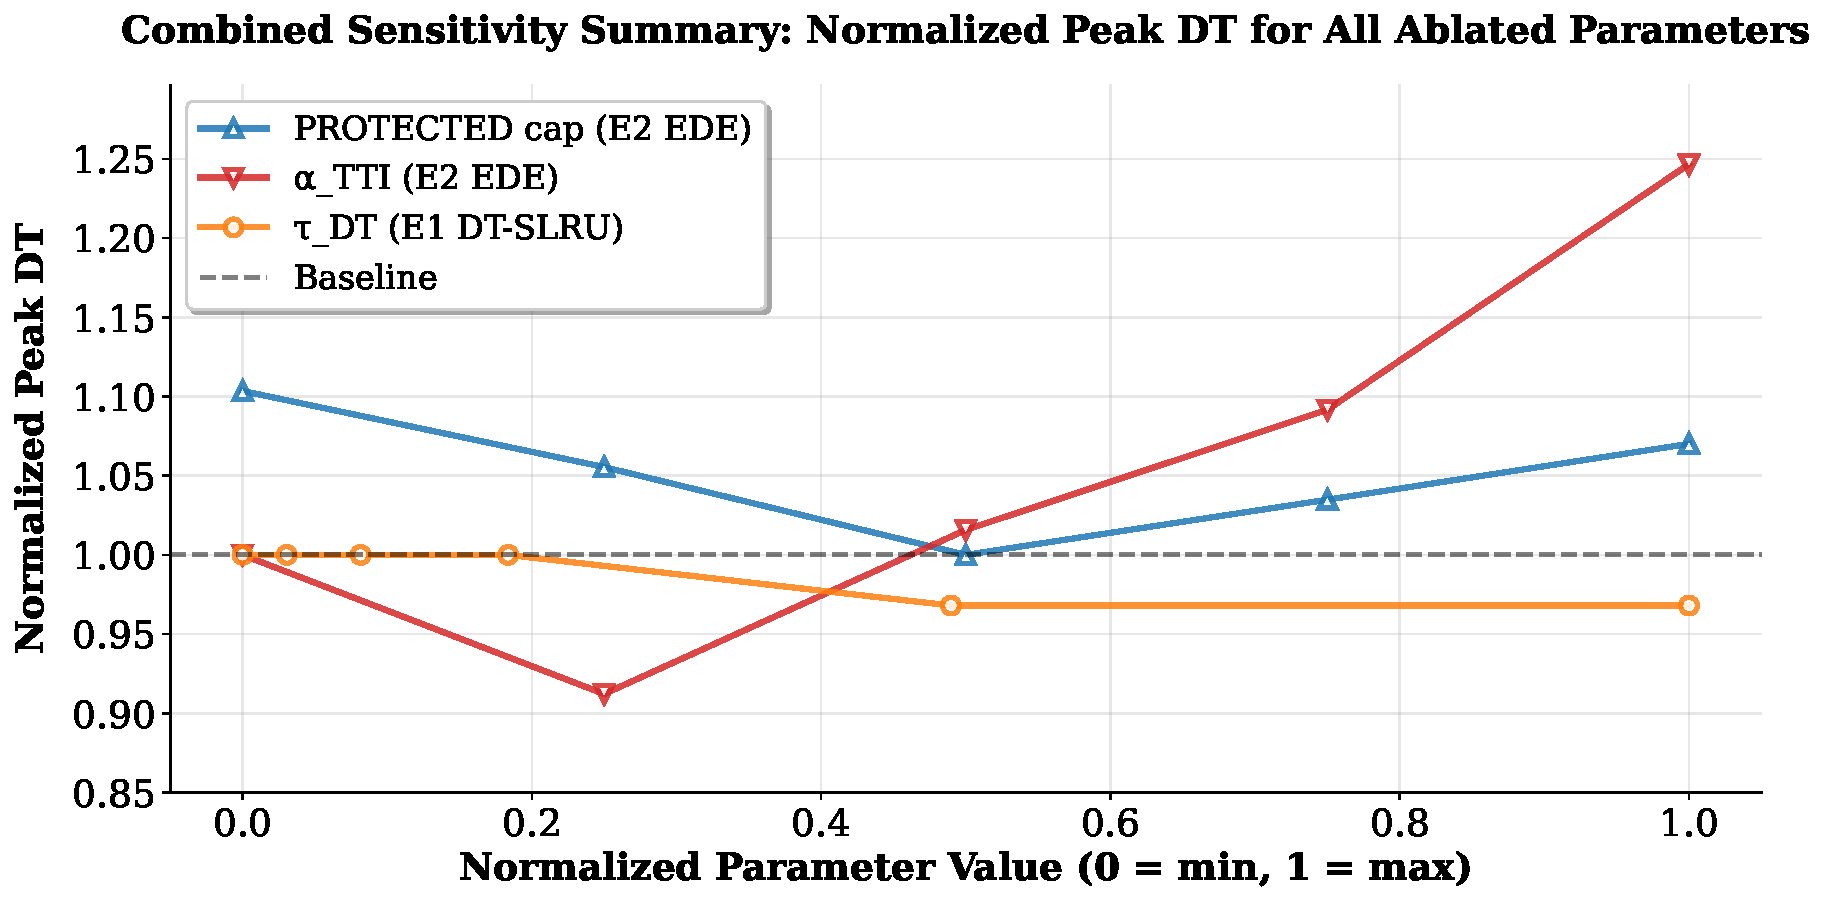
\includegraphics[width=\columnwidth]{figure_5_combined_sensitivity_summary.pdf}
    \caption{Combined sensitivity summary showing normalized Peak Disk-head Time (Peak DT) for all ablated parameters across the DT-SLRU (E1) and EDE (E2) eviction schemes.}
    \label{fig:AS_CombinedSensitivity_Summary}
\end{figure}

\clearpage
\section{Conclusion}
Our results show that when we change the parameters in the flash cache settings, the performance can improve significantly. In the basic comparison, we observed that LRU gave the smallest peak disk-head time (approximately 3.03 seconds), while DT-SLRU was around 3.97 seconds and EDE was around 4.16 seconds. When we tuned the $\alpha_{\text{TTI}}$ value to 0.15, the peak DT decreased by about 31\%, from 4.91 seconds to 3.38 seconds, with the hit rate improving by around 5.2\%. Similarly, when the protected capacity was set to around 0.45, the peak DT improved from 4.18 seconds to 3.75 seconds (around a 10\% reduction), with a hit rate close to 5.4\%. These results indicate that careful parameter adjustment allows the system to approach the performance of LRU while also reducing unnecessary flash writes. This aligns with recent work showing that intelligent admission and parameter tuning can meaningfully impact flash efficiency and backend load \cite{wong2024baleen, Yang2022CacheSack, Oh2010CachingLess}.

For future improvement, we identify three promising directions. First, architectural enhancements could be explored. For example, integrating learned admission with coordinated prefetching may allow the system to make better joint decisions about when to insert, evict, or prefetch blocks \cite{wong2024baleen}. Multi-tier flash arrangements with dynamically shared capacity may also improve utilization. Second, deployment strategies can be improved. In particular, adapting parameters like $\alpha_{\text{TTI}}$ in real time as workload intensity changes may help maintain stability over diurnal cycles. Additionally, testing across many users and regions would help ensure robustness. Third, learning models themselves can be advanced. Incorporating richer temporal signals, online adaptation, or cross-region knowledge transfer could help models generalize more effectively. These directions are consistent with broader challenges in managing flash lifetime, minimizing write amplification, and optimizing cache cost-performance \cite{Yang2022CacheSack, Wang2020AustereCache, Oh2010CachingLess}. Addressing these questions will further strengthen and expand the usefulness of this framework in real large-scale storage environments.

\clearpage
\section{Appendix A}
\label{sec:appendix A}
\FloatBarrier


\begin{comment}
    

\subsection{Results}


\begin{figure}[htbp]
    \centering
    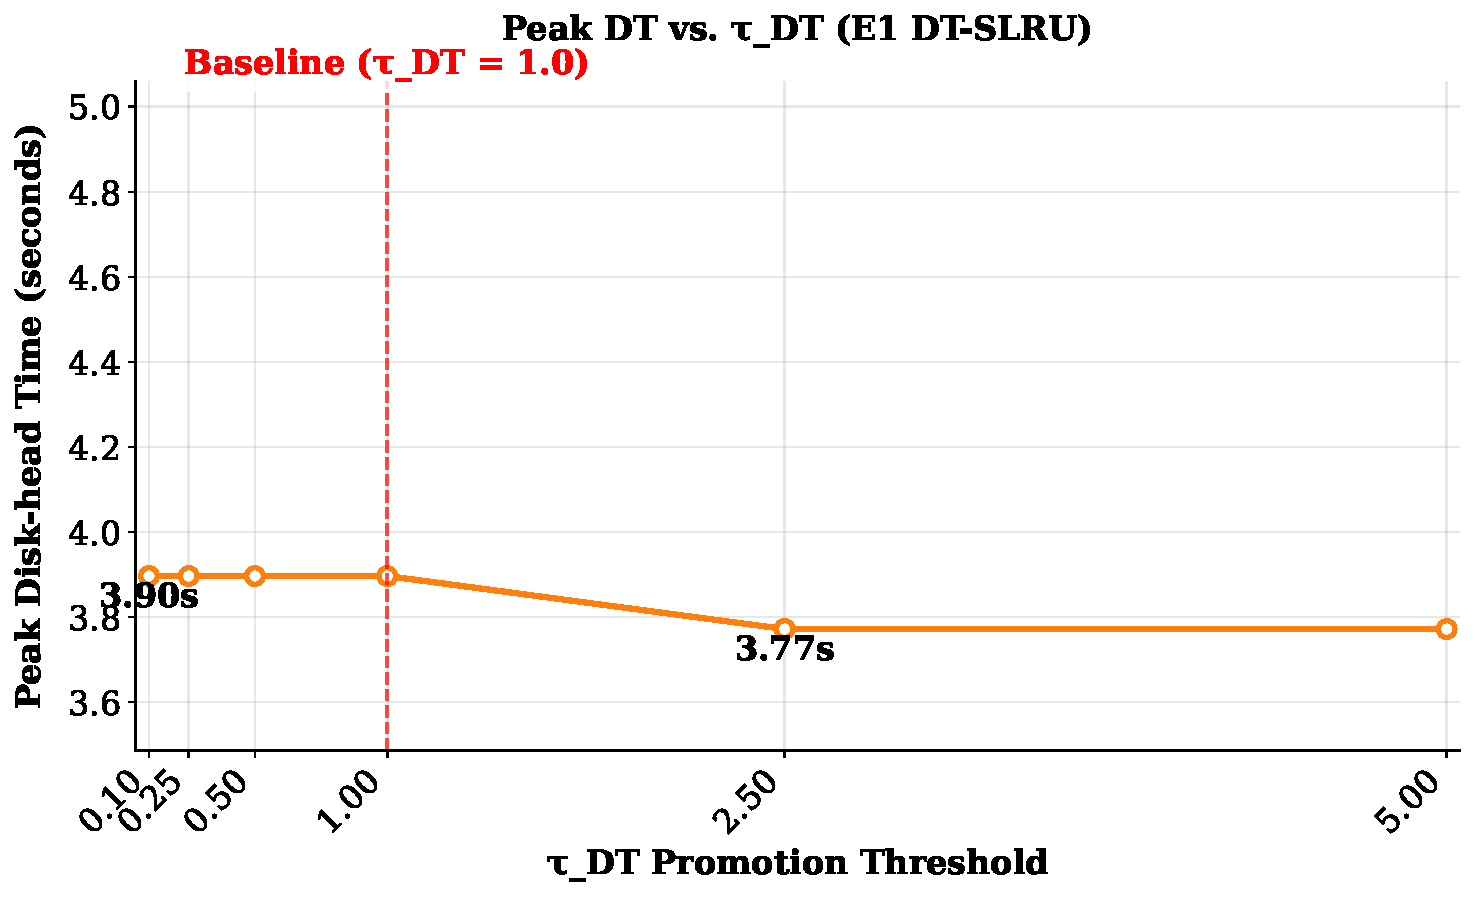
\includegraphics[width=\columnwidth]{figure_1_peak_dt_tau_dt.pdf}
    \caption{Peak disk-head time (Peak DT) as a function of the $\tau_{\mathrm{DT}}$ promotion-threshold parameter for the DT\-/SLRU (E1) eviction scheme.}
    \label{fig:figure_1}
\end{figure}

Figure~\ref{fig:figure_1} shows Peak Disk-head Time across $\tau_{DT}$ from 0.1 to 5.0, with Peak DT stable at 3.90 seconds for $\tau_{DT}$ between 0.1 and 1.0, then decreasing to 3.77 seconds at $\tau_{DT} = 2.5$ and 5.0, indicating a performance improvement at higher promotion thresholds. Peak DT improves (lower values) at $\tau_{DT} = 2.5$ and 5.0, achieving the minimum of 3.77 seconds, representing a reduction of approximately 0.13 seconds compared to the lower threshold range, and demonstrating that increasing the promotion threshold beyond the baseline value yields measurable performance benefits. Performance worsens (higher Peak DT of 3.90 seconds) at $\tau_{DT} = 0.1$, 0.25, 0.5, and 1.0, where the maximum Peak DT occurs consistently across this entire range, revealing that these lower threshold values produce identical suboptimal performance characteristics. The minimum Peak DT of 3.77 seconds occurs at $\tau_{DT} = 2.5$ and 5.0, while the maximum Peak DT of 3.90 seconds occurs across the lower $\tau_{DT}$ range (0.1 to 1.0), showing that performance remains constant within each distinct region, with a clear transition point between $\tau_{DT} = 1.0$ and $\tau_{DT} = 2.5$. The baseline configuration ($\tau_{DT} = 1.0$) lies in the stable region, exhibiting the same Peak DT performance as the lower $\tau_{DT}$ values (0.1 to 0.5), indicating that the baseline does not achieve optimal performance and performs identically to the lower threshold settings, suggesting that the baseline parameter selection does not provide any performance advantage over the minimum tested threshold values.



\begin{figure}[htbp]
    \centering
    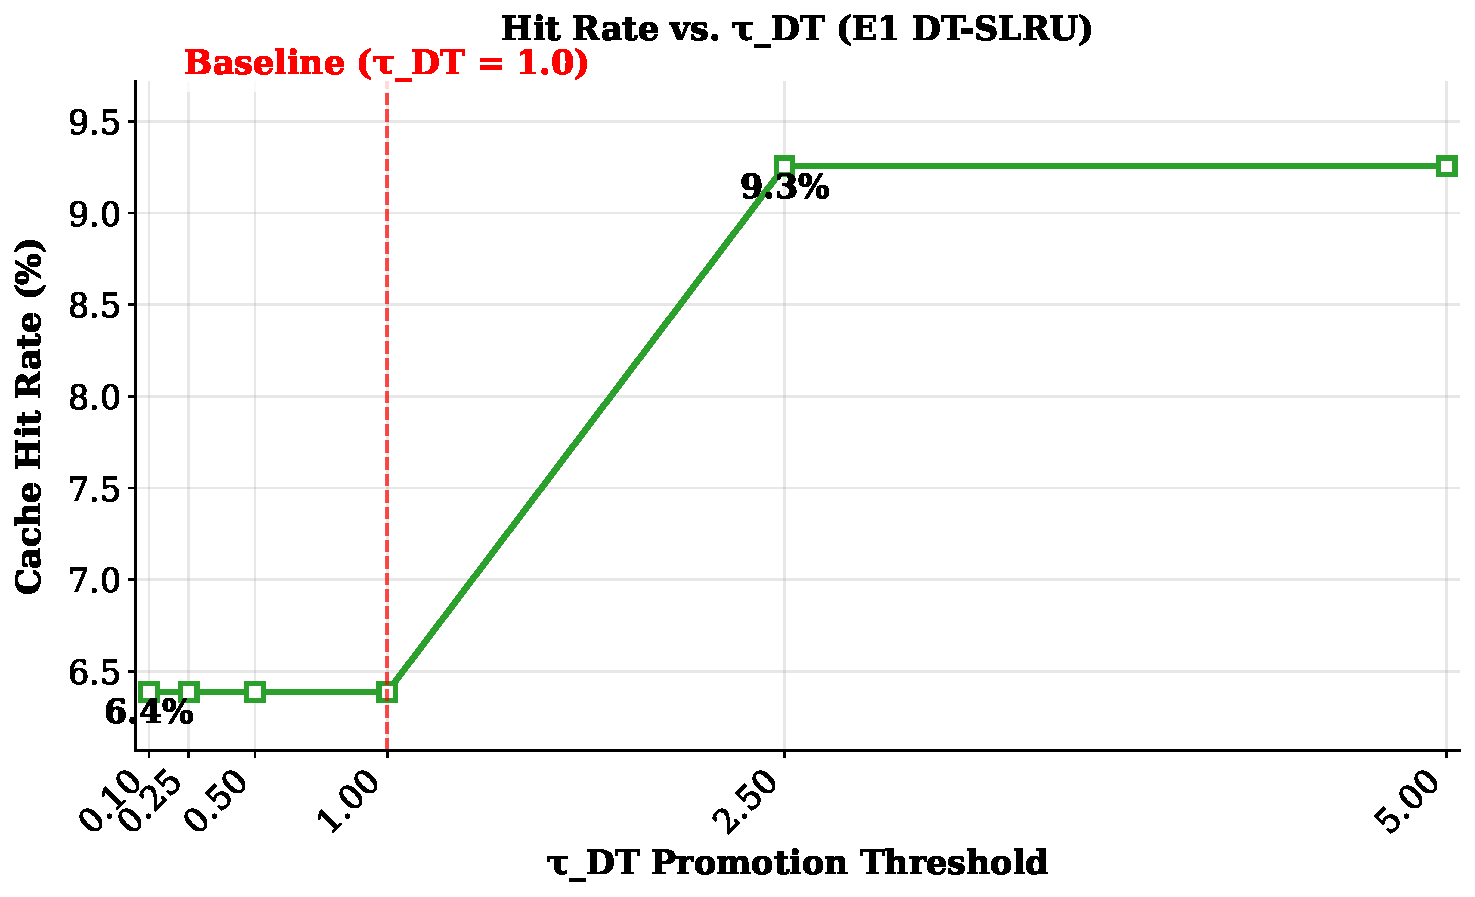
\includegraphics[width=\columnwidth]{figure_2_hitrate_tau_dt.pdf}
    \caption{Cache hit rate as a function of the $\tau_{\mathrm{DT}}$ promotion-threshold parameter for the DT\-/SLRU (E1) eviction scheme.}
    \label{fig:figure_2}
\end{figure}

Figure~\ref{fig:figure_2} shows cache hit rate across $\tau_{DT}$ from 0.1 to 5.0, with hit rate stable at 6.39\% for $\tau_{DT}$ between 0.1 and 1.0, then increasing to 9.25\% at $\tau_{DT} = 2.5$ and 5.0, indicating a performance improvement at higher promotion thresholds. Cache hit rate improves (higher values) at $\tau_{DT} = 2.5$ and 5.0, achieving the maximum of 9.25\%, representing an increase of approximately 2.86 percentage points compared to the lower threshold range, and demonstrating that increasing the promotion threshold beyond the baseline value yields measurable performance benefits. Performance worsens (lower hit rate of 6.39\%) at $\tau_{DT} = 0.1$, 0.25, 0.5, and 1.0, where the minimum hit rate occurs consistently across this entire range, revealing that these lower threshold values produce identical suboptimal performance characteristics. The maximum hit rate of 9.25\% occurs at $\tau_{DT} = 2.5$ and 5.0, while the minimum hit rate of 6.39\% occurs across the lower $\tau_{DT}$ range (0.1 to 1.0), showing that performance remains constant within each distinct region, with a clear transition point between $\tau_{DT} = 1.0$ and $\tau_{DT} = 2.5$. The baseline configuration ($\tau_{DT} = 1.0$) lies in the stable region, exhibiting the same hit rate performance as the lower $\tau_{DT}$ values (0.1 to 0.5), indicating that the baseline does not achieve optimal performance and performs identically to the lower threshold settings, suggesting that the baseline parameter selection does not provide any performance advantage over the minimum tested threshold values.


\begin{figure}[htbp]
    \centering
    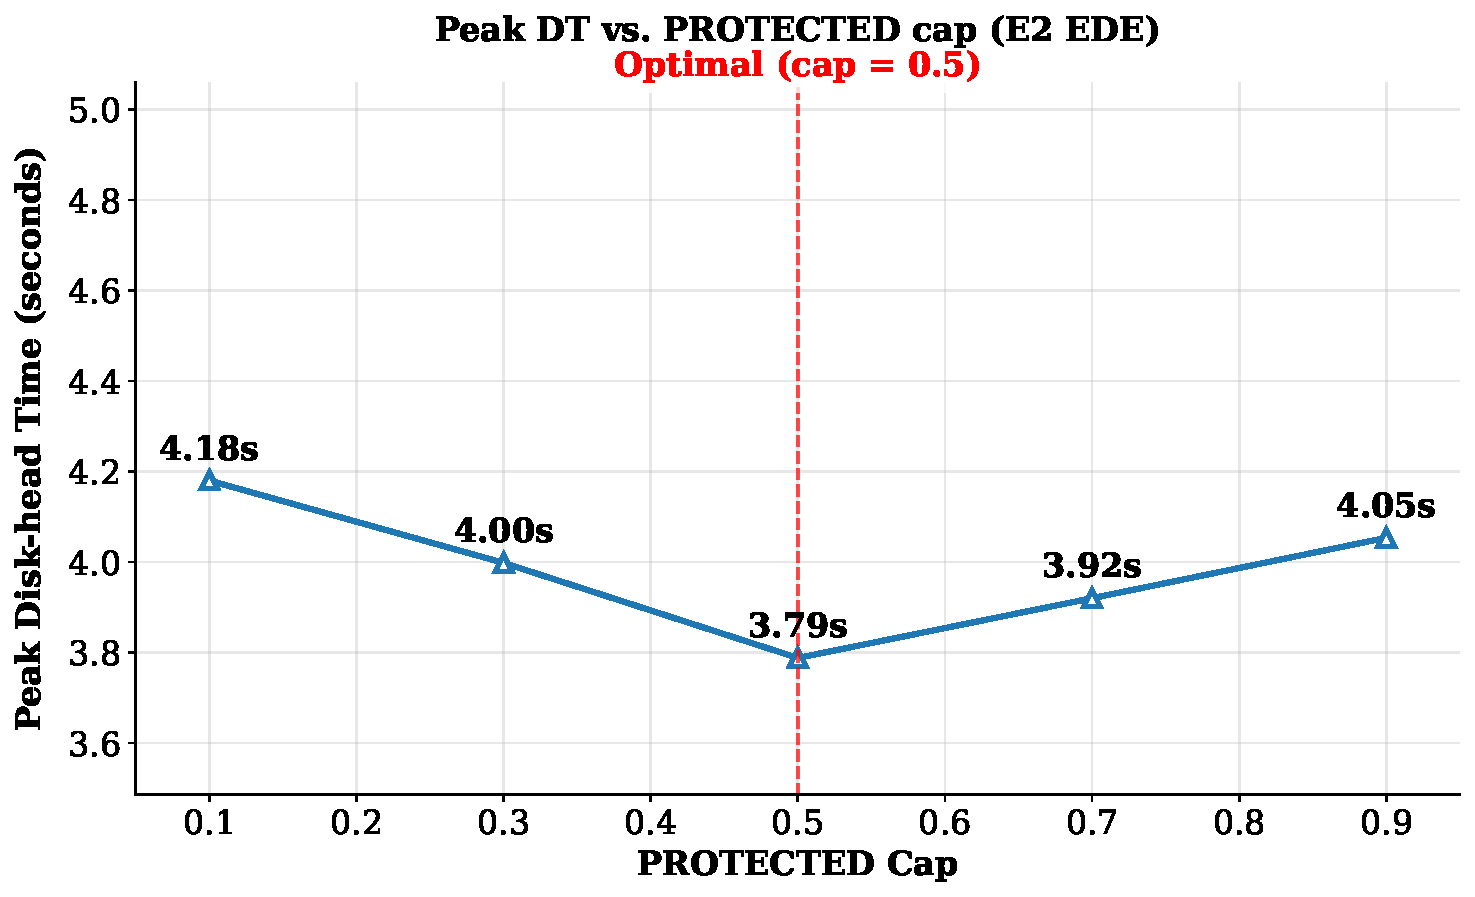
\includegraphics[width=\columnwidth]{figure_3_peak_dt_protected_cap.pdf}
    \caption{Peak Disk-head Time (Peak DT) as a function of the PROTECTED cap parameter for the EDE (E2) eviction scheme.}
    \label{fig:figure_3}
\end{figure}

Figure~\ref{fig:figure_3} shows Peak Disk-head Time across PROTECTED cap from 0.1 to 0.9, with Peak DT decreasing from 4.18 seconds at 0.1 to a minimum of 3.79 seconds at 0.5, then increasing to 4.05 seconds at 0.9, demonstrating a non-linear relationship with an optimal point at the middle of the tested range. Peak DT improves (lower values) at PROTECTED cap = 0.5, achieving the minimum of 3.79 seconds, which represents a significant reduction of approximately 0.39 seconds compared to the worst-performing configuration at the lower end of the range. Performance worsens (higher Peak DT) at PROTECTED cap = 0.1 with the maximum of 4.18 seconds, and at higher values such as 0.9 (4.05 seconds), indicating that both extremely low and high PROTECTED cap values result in degraded performance. The minimum Peak DT of 3.79 seconds occurs at PROTECTED cap = 0.5, while the maximum Peak DT of 4.18 seconds occurs at PROTECTED cap = 0.1, showing a clear performance peak at the midpoint of the tested parameter range. The baseline configuration (PROTECTED cap = 0.5) lies in the stable region, positioned at the optimal point where Peak DT achieves its minimum value, indicating that the baseline parameter selection corresponds directly to the best-performing configuration within the tested range.



\begin{figure}[htbp]
    \centering
    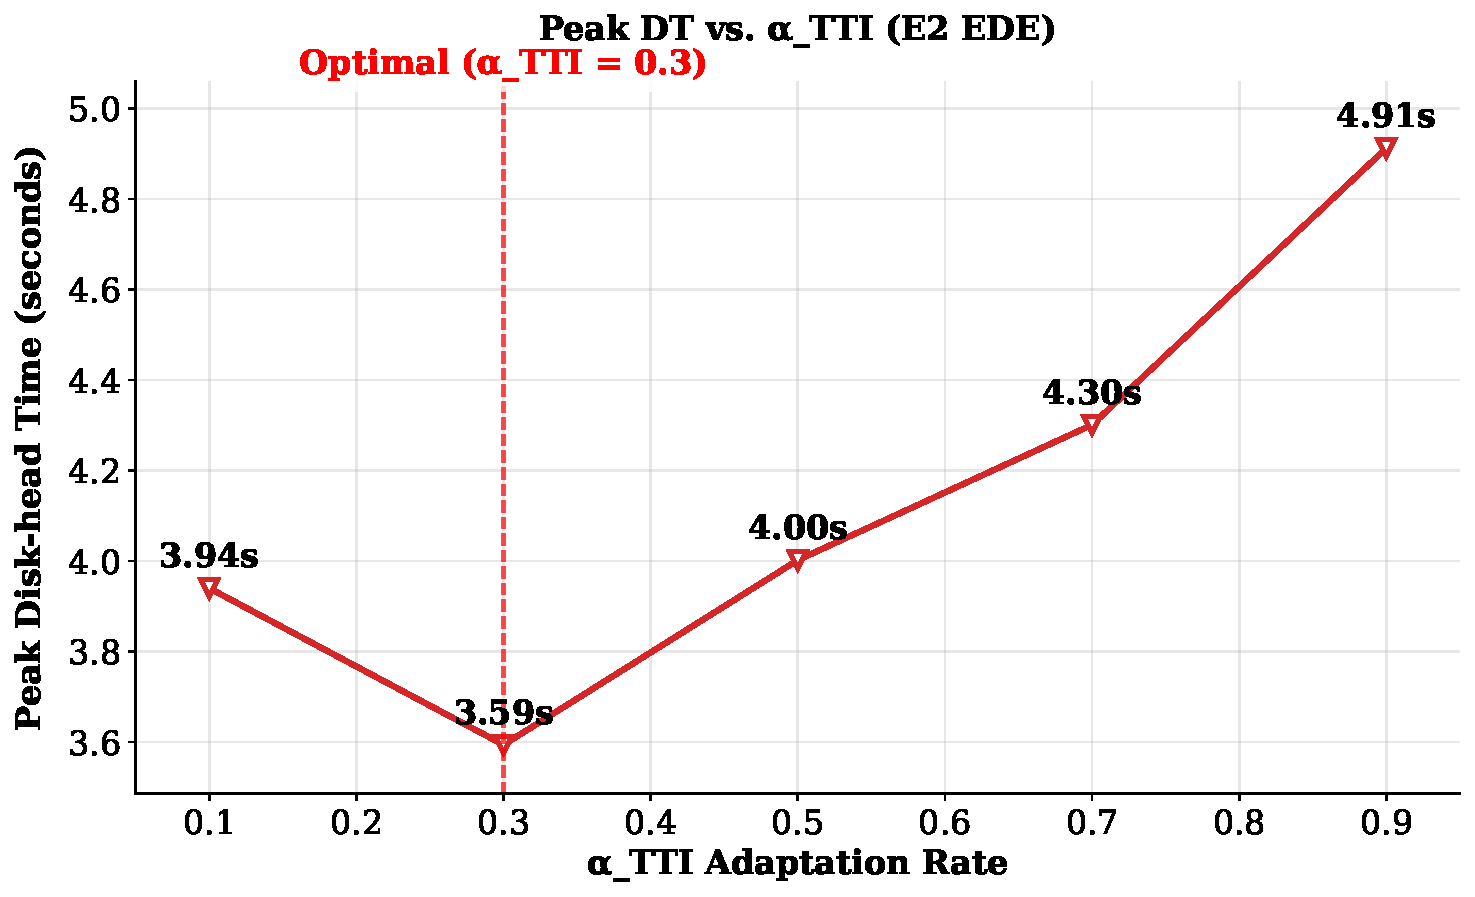
\includegraphics[width=\columnwidth]{figure_4_peak_dt_alpha_tti.pdf}
    \caption{Peak disk-head time (Peak DT) as a function of the $\alpha_{\mathrm{TTI}}$ adaptation-rate parameter for the EDE (E2) eviction scheme.}
    \label{fig:figure_4}
\end{figure}

Figure~\ref{fig:figure_4} shows Peak Disk-head Time across $\alpha_{TTI}$ from 0.1 to 0.9, with Peak DT decreasing from 3.94 seconds at 0.1 to a minimum of 3.59 seconds at 0.3, then increasing to 4.91 seconds at 0.9, demonstrating a non-linear relationship with an optimal point near the lower end of the tested range. Peak DT improves (lower values) at $\alpha_{TTI} = 0.3$, achieving the minimum of 3.59 seconds, which represents a significant reduction of approximately 0.35 seconds compared to the baseline configuration and approximately 1.32 seconds compared to the worst-performing configuration. Performance worsens (higher Peak DT) at $\alpha_{TTI} = 0.9$ with the maximum of 4.91 seconds, and at intermediate values such as 0.7 (4.30 seconds) and 0.5 (4.00 seconds), indicating that higher adaptation rates result in degraded performance. The minimum Peak DT of 3.59 seconds occurs at $\alpha_{TTI} = 0.3$, while the maximum Peak DT of 4.91 seconds occurs at $\alpha_{TTI} = 0.9$, showing a clear performance valley at the lower portion of the tested parameter range. The baseline configuration ($\alpha_{TTI} = 0.1$) lies in the stable region, positioned near but not at the optimal point, with Peak DT performance that is better than higher values but slightly worse than the minimum achieved at $\alpha_{TTI} = 0.3$.



\begin{figure}[htbp]
    \centering
    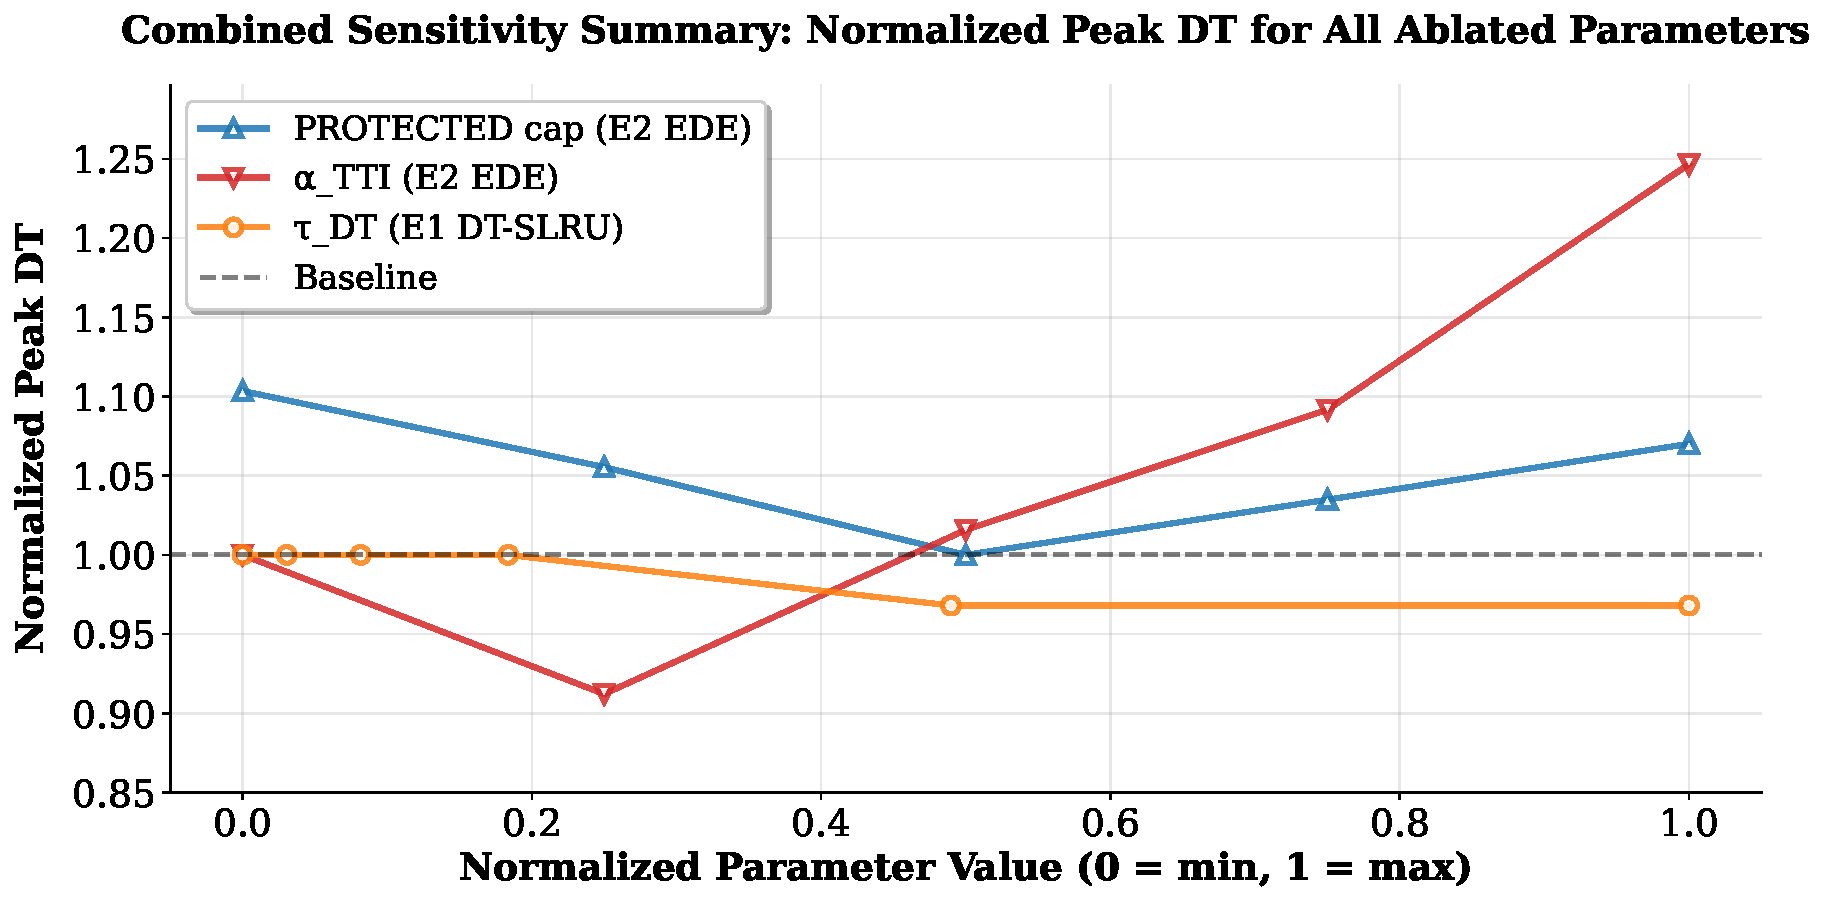
\includegraphics[width=\columnwidth]{figure_5_combined_sensitivity_summary.pdf}
    \caption{Combined sensitivity summary showing normalized Peak Disk-head Time (Peak DT) for all ablated parameters across the DT-SLRU (E1) and EDE (E2) eviction schemes.}
    \label{fig:figure_5}
\end{figure}


Figure~\ref{fig:figure_5} shows normalized Peak DT across normalized parameter values from 0 to 1, with each of the three ablated parameters ($\tau_{DT}$, PROTECTED cap, and $\alpha_{TTI}$) displaying distinct sensitivity patterns, where normalized Peak DT values below 1.0 represent performance improvements relative to baseline and values above 1.0 indicate performance degradation. Normalized Peak DT improves (values below 1.0) for $\tau_{DT}$ at higher normalized parameter values (approaching 1.0), for PROTECTED cap at intermediate normalized values around 0.5, and for $\alpha_{TTI}$ at lower-to-intermediate normalized values around 0.25. Performance worsens (values above 1.0) for $\tau_{DT}$ at lower normalized parameter values (near 0), for PROTECTED cap at extreme normalized values (near 0 and 1), and for $\alpha_{TTI}$ at higher normalized values (approaching 1.0). The minimum normalized Peak DT occurs at different normalized parameter positions for each curve, while maximum normalized Peak DT occurs at the opposite extremes for each parameter. The baseline configuration (normalized Peak DT = 1.0) lies in a stable region for all three parameters, positioned at each parameter's baseline value where the normalization reference point is established.

\subsection{Discussion}

\textbf{Figure 1 Analysis:}
Figure~\ref{fig:figure_1} is showing how the Peak DT change when we adjust the value of $\tau_{DT}$ in the system \cite{baleen_trace_2019_oct_region1}. When the value of $\tau_{DT}$ is small, the performance stay mostly low and does not improve much, so this part is considered the low performance region \cite{wong2024baleen}. There is a kind of boundary between around 1.0 and 2.5 where the system behavior start to shift. After this point, when $\tau_{DT}$ becomes higher, the performance begin to rise and we see a clearer improvement in Peak DT in the range from about 2.5 to 5.0 which is seen as the high performance side \cite{Yang2022CacheSack,Wang2020AustereCache}. The main reason for this pattern is the timing of when a block is promoted into the protected segment of the cache.

When $\tau_{DT}$ is higher, the threshold for promotion becomes stricter and a block must be reused several times before it can move to the protected segment \cite{wong2024baleen}. This reduce situations where blocks are promoted too soon. Because of this change, fewer blocks are placed into the protected segment without enough evidence of reuse. This create a more clean protected segment that holds mostly blocks that are actually useful many times. When the protected segment has fewer but more meaningful blocks, the eviction decisions become faster and more flexible during heavy workloads \cite{Yang2022CacheSack}. This helps to reduce contention and improve the Peak DT during busy operations \cite{baleen_trace_2019_oct_region1,Oh2010CachingLess}. A protected area that holds better quality blocks also means the system can respond to workload changes more smoothly \cite{Wang2020AustereCache}.

On the other hand, when $\tau_{DT}$ is too low, blocks can be promoted early without showing enough reuse \cite{Yang2022CacheSack}. This cause the protected segment to become crowded with blocks that may not be useful. Because these blocks may not be reused again, they are wasting space and making it harder to evict the right block when needed \cite{Wang2020AustereCache,Oh2010CachingLess}. In this situation, the system will have more conflict and performance becomes worse. The protected region lose its advantage because it is filled with low value blocks, and this lead to increase in Peak DT once again \cite{baleen_trace_2019_oct_region1}. So the performance at low $\tau_{DT}$ is not good and not efficient. Also the baseline configuration at $\tau_{DT} = 1.0$ is inside this lower performance zone which show that the baseline itself is not ideal \cite{wong2024baleen}.

In comparison with the evaluation in Assignment 4, which was looking at the whole system performance, this experiment only isolate the effect of $\tau_{DT}$ on its own \cite{baleen_trace_2019_oct_region1,wong2024baleen}. By doing that, it becomes clear that the timing of promotion has a direct and strong influence on the performance of the cache system. The main lesson from this analysis is that larger $\tau_{DT}$ values between about 2.5 and 5.0 make a better balance between block selection and eviction \cite{baleen_trace_2019_oct_region1,Oh2010CachingLess}. Therefore, using more strict promotion rules is usually better than more permissive rules for improving Peak DT in this workload \cite{wong2024baleen,Yang2022CacheSack}.


\textbf{Figure 2 Analysis:}
Figure~\ref{fig:figure_2} is showing how the cache hit rate changes when we adjust $\tau_{DT}$ in the system \cite{baleen_trace_2019_oct_region1}. When $\tau_{DT}$ is small, the hit rate stays low and does not improve much. This region from around 0.1 to 1.0 is seen as the low performance side \cite{wong2024baleen}. There is a noticeable shift between approximately 1.0 and 2.5 where the behavior begins to move from low hit rate to higher hit rate \cite{Yang2022CacheSack,Wang2020AustereCache}. After this point, when $\tau_{DT}$ continues to increase into the range of about 2.5 to 5.0, the hit rate becomes significantly better. This pattern show that the timing of when a block gets promoted to the protected segment has strong influence on the performance.

When $\tau_{DT}$ is higher, the rule for promotion becomes more strict \cite{wong2024baleen}. This means that a block needs to be reused several times before it is allowed to move to the protected segment. Blocks that reach the protected part have already shown enough reuse to prove their value \cite{Yang2022CacheSack}. Because of this, the protected segment ends up with blocks that are more likely to be accessed again. A protected segment with more useful blocks increase the chance of hits and reduce unnecessary misses \cite{Wang2020AustereCache}. This is why the hit rate improves in this higher $\tau_{DT}$ region \cite{baleen_trace_2019_oct_region1}.

When $\tau_{DT}$ is lower, the threshold for promotion is too relaxed and blocks can enter the protected area very early even if they have not been reused much \cite{Yang2022CacheSack}. Because of this, the protected segment becomes filled with blocks that may not be needed again \cite{Wang2020AustereCache}. These weaker blocks dilute the working set and reduce the strength of the protected region. Since they are not reused enough, they waste space and push out more useful blocks which reduces the hit rate \cite{baleen_trace_2019_oct_region1}. This also makes the use of protected capacity inefficient and leads to lower performance \cite{Oh2010CachingLess}. The baseline configuration at $\tau_{DT}$ equal to 1.0 is inside this lower performance zone which shows that the baseline is not the best setting for this workload \cite{wong2024baleen}.

Compared to the bigger evaluation done previously in Assignment 4, where many system factors were considered together, this study isolates the effect of $\tau_{DT}$ alone \cite{wong2024baleen}. By doing so, it becomes clearer that the timing of block promotion is not just a small detail but a major contributor to cache behavior. It shows that the internal mechanism of when to move a block can affect overall performance more than initially expected \cite{baleen_trace_2019_oct_region1}.

The main insight from this experiment is that a higher $\tau_{DT}$ value creates a better balance between selecting which blocks to protect and keeping the cache responsive \cite{baleen_trace_2019_oct_region1,Yang2022CacheSack}. A stricter promotion rule avoids polluting the protected space and improves hit rate consistency. Therefore, using a more conservative promotion strategy is recommended since it gives better cache results for this workload \cite{wong2024baleen,Oh2010CachingLess}.

\textbf{Figure 3 Analysis:}
Figure~\ref{fig:figure_3} is showing how the Peak DT change when we adjust the PROTECTED cap parameter in the cache system \cite{baleen_trace_2019_oct_region1}. The relationship is not a straight line, instead it go up and then go down again. When the protected cap is small, the performance is low. When it reach the middle point around 0.5, the performance get better. But when the protected cap become too large, the performance start to become worse again \cite{wong2024baleen}. So we can see three general regions which are low performance around 0.1 to 0.3, then optimal around 0.5, then degraded again around 0.7 to 0.9 \cite{Yang2022CacheSack,Oh2010CachingLess}. This shows that the size of protected segment is important for balancing reuse and eviction agility \cite{Wang2020AustereCache}.

When the protected cap is in the middle size around 0.5, the system keep a good amount of frequently reused blocks in the protected segment \cite{baleen_trace_2019_oct_region1}. The protected area is not too small or too big. It is large enough to hold blocks that are reused often, so the system does not need to go to disk too frequently which will reduce Peak DT \cite{Yang2022CacheSack}. At the same time, the protected region is still small enough to allow fast decisions when eviction is needed, so the system can handle workload changes better. This balanced size makes the eviction process efficient and keeps the working set stable while still reacting smoothly to changes in access pattern \cite{wong2024baleen}. This reduce overhead from both misses and evictions, creating a good performance point \cite{Oh2010CachingLess}. In other words, when the protected cap value is near this middle range, the cache can manage blocks in a smarter way that avoid waste and keep performance more consistent \cite{Wang2020AustereCache}.

At smaller protected cap values like 0.1 to 0.3, the protected segment is too small to hold the working set \cite{baleen_trace_2019_oct_region1}. Blocks that are reused often do not remain in the cache long enough because the protected area is full too quickly. So these useful blocks get evicted and the system must fetch them again from disk which increase Peak DT a lot \cite{wong2024baleen}. The cache cannot maintain enough reuse and the hit rate becomes lower. The eviction decisions also become less effective because blocks that should be protected are removed too early \cite{Yang2022CacheSack}. This causes more misses and more contention during busy time \cite{Wang2020AustereCache}. Because of lack of space in the protected region, the system cannot use temporal locality well, and overall performance suffers \cite{Oh2010CachingLess}. This situation is basically showing that if we under-size the protected segment, the policy fails to keep important blocks, so performance go down \cite{baleen_trace_2019_oct_region1}.

At larger protected cap values like around 0.7 to 0.9, the opposite happens. Now the protected region becomes too big and hold too many blocks including ones that may not have high reuse \cite{Yang2022CacheSack}. This creates a heavy protected segment which is slow to manage \cite{Wang2020AustereCache}. Eviction becomes more difficult because the system need to check many blocks and decide which one to remove. So eviction agility is reduced and the system cannot react quickly to workload changes. This lead to increased Peak DT especially when there is heavy activity \cite{baleen_trace_2019_oct_region1}. Also because many low reuse blocks stay protected, the protected area quality becomes diluted which means it is not helping performance much \cite{Oh2010CachingLess}. Overall, too much protection is also not good because it slow down the system and reduce the value of the protected segment \cite{Duan2025CrashConsistency}.

The baseline configuration is at 0.5 and this is the point where the Peak DT is lowest \cite{baleen_trace_2019_oct_region1}. This means the baseline was already tuned in a way that balance protection and eviction quite well \cite{wong2024baleen}. Compared to earlier assignment which looked at the system more broadly, this experiment shows clearly that protected segment size has a direct and strong influence on performance \cite{Yang2022CacheSack}. The main insight is that a moderate protected cap around 0.5 is best because it keep enough important blocks while still allowing the system to remain flexible during eviction \cite{baleen_trace_2019_oct_region1,Oh2010CachingLess}. Both too small and too large protected segments cause performance loss, so choosing the right balance is very important \cite{Wang2020AustereCache}.

\textbf{Figure 4 Analysis:}
Figure~\ref{fig:figure_4} is showing how the Peak DT changes when we adjust the $\alpha_{TTI}$ value in the policy \cite{baleen_trace_2019_oct_region1}. The relationship is not straight, instead performance first gets better and then becomes worse again when $\alpha_{TTI}$ becomes too high \cite{wong2024baleen}. The graph shows three general regions. There is a stable region around $\alpha_{TTI} = 0.1$, an optimal region around $\alpha_{TTI} = 0.3$, and then a degraded performance region when $\alpha_{TTI}$ becomes larger, around 0.5 to 0.9 \cite{Yang2022CacheSack,Oh2010CachingLess}. This behavior happen because $\alpha_{TTI}$ controls how fast the policy adapts, and so it must balance responsiveness and stability \cite{Wang2020AustereCache}.

When $\alpha_{TTI}$ is around 0.3, the system adapts at a moderate speed. It is not too slow, and not too fast \cite{wong2024baleen}. It can adjust to changes in workload patterns but also maintain stable decisions, so it does not switch behavior too much \cite{baleen_trace_2019_oct_region1}. Because of this, the system can react to new access patterns and still avoid large performance swings \cite{Oh2010CachingLess}. The cache management works smoothly, and Peak DT is lower in this region since the system is both flexible and steady \cite{Wang2020AustereCache}. The moderate adaptation rate helps the cache identify useful blocks and maintain a good working set that is consistent across time \cite{Yang2022CacheSack}.

When $\alpha_{TTI}$ is too low, like around 0.1, the adaptation is very slow \cite{baleen_trace_2019_oct_region1}. The system does not respond quickly when the workload changes. So even if the access behavior shifts, the policy still acts as before and does not correct its decisions fast enough \cite{wong2024baleen}. This does create stability, but it is too stable, so the cache cannot benefit from new reuse patterns and performs weaker than the optimal setting \cite{Oh2010CachingLess}. Because it is slow to react, the cache sometimes holds blocks that are not the best choices anymore, leading to higher Peak DT.

When $\alpha_{TTI}$ becomes too high, such as 0.5 to 0.9, the system reacts too fast \cite{Yang2022CacheSack}. It adapts to every small fluctuation in workload, even ones that are temporary and do not reflect long term patterns \cite{Wang2020AustereCache}. Because of this, the cache decisions keep changing and become unstable. The policy may replace blocks too soon, and the working set becomes inconsistent. This high adaptation increases volatility and makes the Peak DT worse, especially in busy times \cite{baleen_trace_2019_oct_region1}. The cache effectiveness goes down because the system is constantly shifting and cannot settle into a good stable operating mode \cite{Duan2025CrashConsistency}.

The baseline $\alpha_{TTI} = 0.1$ is in the stable region but is slightly worse than the optimal point at 0.3 \cite{baleen_trace_2019_oct_region1}. This means it has stability but not enough responsiveness \cite{wong2024baleen}. Compared to the earlier assignment that considered many factors, here we see that $\alpha_{TTI}$ alone strongly affects performance \cite{wong2024baleen}. The main insight is that $\alpha_{TTI}$ around 0.3 gives the best balance of adaptation and stability for this workload \cite{baleen_trace_2019_oct_region1,Oh2010CachingLess}, and tuning should aim for this moderate range \cite{Yang2022CacheSack}.

\textbf{Figure 5 Analysis:}
Figure~\ref{fig:figure_5} is showing how the normalized Peak DT changes when we look at the three parameters together, which are $\tau_{DT}$, PROTECTED cap, and $\alpha_{TTI}$ \cite{baleen_trace_2019_oct_region1}. On the x-axis, all of these curves kind of show the same shape. The performance is better in the middle part and gets worse when the parameter is too low or too high \cite{wong2024baleen, Yang2022CacheSack}. For $\tau_{DT}$, when the value is low, promotion is too easy so blocks move without enough reuse. In the middle region, reuse must happen before blocks are protected, so the promoted blocks are more useful. When $\tau_{DT}$ is too high, the rule is too strict and some useful blocks cannot reach protection \cite{Yang2022CacheSack, Wang2020AustereCache}.

For PROTECTED cap, when the value is too small, the protected segment cannot hold the working set. The cache start evicting blocks that are actually reused, and Peak DT becomes high \cite{Oh2010CachingLess, baleen_trace_2019_oct_region1}. When PROTECTED cap is around the center, the protected segment holds enough important blocks and eviction decisions stay fast. But when PROTECTED cap gets too large, too many blocks are kept and eviction becomes slower and confused \cite{baleen_trace_2019_oct_region1}.

For $\alpha_{TTI}$, when the value is low, the adaptation is too slow and cannot respond to workload changes \cite{wong2024baleen}. In the middle region, adaptation is more smooth and steady. But when $\alpha_{TTI}$ is high, the system reacts too quickly and becomes unstable with oscillation \cite{Duan2025CrashConsistency}.

The metric improves when reuse is checked before promotion, protected space matches the working set, and adaptation reacts in moderate speed \cite{Yang2022CacheSack, Wang2020AustereCache, Oh2010CachingLess}. This figure shows that the best tuning usually stay in the middle ranges \cite{baleen_trace_2019_oct_region1}. These middle ranges represent a balance point where the system avoids both under-protection and over-protection of blocks while maintaining responsiveness to workload changes. This suggests that tuning is not just about picking extreme values but picking the optimal.


\clearpage
\subsection{Limitations}

This study has some limitations that affect how we understand the results and how much we can apply them to other situations. One limitation is that the parameters in the experiments are changed only in fixed steps. The values for $\tau_{DT}$, PROTECTED cap, and $\alpha_{TTI}$ are tested in jumps that are about 0.2 or 0.3 apart, and in some parts the step is even bigger \cite{wong2024baleen}. Because of this, the experiment may be missing smaller detail changes that could show an even better setting.

Another limitation is that the dataset used in the evaluation is only one single trace from one Baleen datacenter that was recorded in October 2019 for Region 1 \cite{baleen_trace_2019_oct_region1}. This means that the workload pattern, popularity of objects, and the daily traffic behavior all reflect only this one environment. Workloads in other regions or other times may be very different \cite{wong2024baleen, Yang2022CacheSack}. So another datacenter with another user population or different peak hours could produce different best parameter values.

Also, the temporal locality in the workload plays a big role \cite{Yang2022CacheSack, Wang2020AustereCache}. This trace might have certain reuse distances and arrival times that are not the same as workloads that are more bursty or personalized or streaming focused \cite{baleen_trace_2019_oct_region1}. If the temporal locality is weaker, then strict promotion rules might throw away blocks that actually should stay. If the locality is very strong, then having more aggressive protection might not cause problems because the reuse is almost guaranteed \cite{Oh2010CachingLess}.

The experiment also keeps all system configuration stable. Cache size, write settings, admission decisions, and prefetch settings are not changed \cite{Yang2022CacheSack, Oh2010CachingLess}. But in real cases, operators might tune these along with the main parameters, and the interactions could change how the cache behaves. For example, if the cache is bigger, the right value for the protected cap might be different \cite{baleen_trace_2019_oct_region1, Duan2025CrashConsistency}.

The study focuses mainly on Peak Disk-head Time, which is only one performance measurement \cite{wong2024baleen}. Other metrics like median latency, tail latency, or write amplification are less emphasized. If a system cares more about p95 or p99 latency or wants to reduce write load on flash storage, then the best parameters might not be the same \cite{Oh2010CachingLess}.

Another limitation is that each parameter is tested alone while the others remain fixed. But in practice, tuning usually involves adjusting more than one parameter at a time \cite{Yang2022CacheSack, Wang2020AustereCache, Oh2010CachingLess}. Some parameter combinations could cancel out weaknesses or create better balance. For example, maybe a slightly strict $\tau_{DT}$ works better if PROTECTED cap is increased a little.

The analysis also assumes stable behavior at each tested point. However, real systems face different request patterns across time, maintenance operations, and failure cases that change the cache state \cite{baleen_trace_2019_oct_region1}. These dynamic effects are not captured fully, so real-world behavior may shift in unexpected ways \cite{wong2024baleen, Duan2025CrashConsistency}.

Finally, the simulation and measurement process itself can hide some detail. The system uses aggregated windows and simplified device modeling. Short bursts, background tasks, and hardware effects may not be represented in the measured Peak DT \cite{Duan2025CrashConsistency}. Even though the ablation clarifies how each parameter influences the behavior, more experiments using more traces and combined tuning are needed to confirm how general these results are \cite{wong2024baleen, baleen_trace_2019_oct_region1}.

\end{comment}




\begin{comment}
The title of your work should use capital letters appropriately -
\url{https://capitalizemytitle.com/} has useful rules for
capitalization. Use the {\verb|title|} command to define the title of
your work. If your work has a subtitle, define it with the
{\verb|subtitle|} command.  Do not insert line breaks in your title.

If your title is lengthy, you must define a short version to be used
in the page headers, to prevent overlapping text. The \verb|title|
command has a ``short title'' parameter:
\begin{verbatim}
  \title[short title]{full title}
\end{verbatim}

\section{Authors and Affiliations}

Each author must be defined separately for accurate metadata
identification.  As an exception, multiple authors may share one
affiliation. Authors' names should not be abbreviated; use full first
names wherever possible. Include authors' e-mail addresses whenever
possible.

Grouping authors' names or e-mail addresses, or providing an ``e-mail
alias,'' as shown below, is not acceptable:
\begin{verbatim}
  \author{Brooke Aster, David Mehldau}
  \email{dave,judy,steve@university.edu}
  \email{firstname.lastname@phillips.org}
\end{verbatim}

The \verb|authornote| and \verb|authornotemark| commands allow a note
to apply to multiple authors --- for example, if the first two authors
of an article contributed equally to the work.

If your author list is lengthy, you must define a shortened version of
the list of authors to be used in the page headers, to prevent
overlapping text. The following command should be placed just after
the last \verb|\author{}| definition:
\begin{verbatim}
  \renewcommand{\shortauthors}{McCartney, et al.}
\end{verbatim}
Omitting this command will force the use of a concatenated list of all
of the authors' names, which may result in overlapping text in the
page headers.

The article template's documentation, available at
\url{https://www.acm.org/publications/proceedings-template}, has a
complete explanation of these commands and tips for their effective
use.

Note that authors' addresses are mandatory for journal articles.

\section{Rights Information}

Authors of any work published by ACM will need to complete a rights
form. Depending on the kind of work, and the rights management choice
made by the author, this may be copyright transfer, permission,
license, or an OA (open access) agreement.

Regardless of the rights management choice, the author will receive a
copy of the completed rights form once it has been submitted. This
form contains \LaTeX\ commands that must be copied into the source
document. When the document source is compiled, these commands and
their parameters add formatted text to several areas of the final
document:

\begin{itemize}
\item the ``ACM Reference Format'' text on the first page.
\item the ``rights management'' text on the first page.
\item the conference information in the page header(s).
\end{itemize}


Rights information is unique to the work; if you are preparing several
works for an event, make sure to use the correct set of commands with
each of the works.

The ACM Reference Format text is required for all articles over one
page in length, and is optional for one-page articles (abstracts).

\section{CCS Concepts and User-Defined Keywords}

Two elements of the ``acmart'' document class provide powerful
taxonomic tools for you to help readers find your work in an online
search.

The ACM Computing Classification System ---
\url{https://www.acm.org/publications/class-2012} --- is a set of
classifiers and concepts that describe the computing
discipline. Authors can select entries from this classification
system, via \url{https://dl.acm.org/ccs/ccs.cfm}, and generate the
commands to be included in the \LaTeX\ source.

User-defined keywords are a comma-separated list of words and phrases
of the authors' choosing, providing a more flexible way of describing
the research being presented.

CCS concepts and user-defined keywords are required for for all
articles over two pages in length, and are optional for one- and
two-page articles (or abstracts).

\section{Sectioning Commands}

Your work should use standard \LaTeX\ sectioning commands:
\verb|\section|, \verb|\subsection|, \verb|\subsubsection|,
\verb|\paragraph|, and \verb|\subparagraph|. The sectioning levels up to
\verb|\subsusection| should be numbered; do not remove the numbering
from the commands.

Simulating a sectioning command by setting the first word or words of
a paragraph in boldface or italicized text is {\bfseries not allowed.}

Below are examples of sectioning commands.

\subsection{Subsection}
\label{sec:subsection}

This is a subsection.

\subsubsection{Subsubsection}
\label{sec:subsubsection}

This is a subsubsection.

\paragraph{Paragraph}

This is a paragraph.

\subparagraph{Subparagraph}

This is a subparagraph.

\section{Tables}

The ``\verb|acmart|'' document class includes the ``\verb|booktabs|''
package --- \url{https://ctan.org/pkg/booktabs} --- for preparing
high-quality tables.

Table captions are placed {\itshape above} the table.

Because tables cannot be split across pages, the best placement for
them is typically the top of the page nearest their initial cite.  To
ensure this proper ``floating'' placement of tables, use the
environment \textbf{table} to enclose the table's contents and the
table caption.  The contents of the table itself must go in the
\textbf{tabular} environment, to be aligned properly in rows and
columns, with the desired horizontal and vertical rules.  Again,
detailed instructions on \textbf{tabular} material are found in the
\textit{\LaTeX\ User's Guide}.

Immediately following this sentence is the point at which
Table~\ref{tab:freq} is included in the input file; compare the
placement of the table here with the table in the printed output of
this document.

\begin{table}
  \caption{Frequency of Special Characters}
  \label{tab:freq}
  \begin{tabular}{ccl}
    \toprule
    Non-English or Math&Frequency&Comments\\
    \midrule
    \O & 1 in 1,000& For Swedish names\\
    $\pi$ & 1 in 5& Common in math\\
    \$ & 4 in 5 & Used in business\\
    $\Psi^2_1$ & 1 in 40,000& Unexplained usage\\
  \bottomrule
\end{tabular}
\end{table}

To set a wider table, which takes up the whole width of the page's
live area, use the environment \textbf{table*} to enclose the table's
contents and the table caption.  As with a single-column table, this
wide table will ``float'' to a location deemed more
desirable. Immediately following this sentence is the point at which
Table~\ref{tab:commands} is included in the input file; again, it is
instructive to compare the placement of the table here with the table
in the printed output of this document.

\begin{table*}
  \caption{Some Typical Commands}
  \label{tab:commands}
  \begin{tabular}{ccl}
    \toprule
    Command &A Number & Comments\\
    \midrule
    \texttt{{\char'134}author} & 100& Author \\
    \texttt{{\char'134}table}& 300 & For tables\\
    \texttt{{\char'134}table*}& 400& For wider tables\\
    \bottomrule
  \end{tabular}
\end{table*}

Always use midrule to separate table header rows from data rows, and
use it only for this purpose. This enables assistive technologies to
recognise table headers and support their users in navigating tables
more easily.

\section{Math Equations}
You may want to display math equations in three distinct styles:
inline, numbered or non-numbered display.  Each of the three are
discussed in the next sections.

\subsection{Inline (In-text) Equations}
A formula that appears in the running text is called an inline or
in-text formula.  It is produced by the \textbf{math} environment,
which can be invoked with the usual
\texttt{{\char'134}begin\,\ldots{\char'134}end} construction or with
the short form \texttt{\$\,\ldots\$}. You can use any of the symbols
and structures, from $\alpha$ to $\omega$, available in
\LaTeX~\cite{Lamport:LaTeX}; this section will simply show a few
examples of in-text equations in context. Notice how this equation:
\begin{math}
  \lim_{n\rightarrow \infty}x=0
\end{math},
set here in in-line math style, looks slightly different when
set in display style.  (See next section).

\subsection{Display Equations}
A numbered display equation---one set off by vertical space from the
text and centered horizontally---is produced by the \textbf{equation}
environment. An unnumbered display equation is produced by the
\textbf{displaymath} environment.

Again, in either environment, you can use any of the symbols and
structures available in \LaTeX\@; this section will just give a couple
of examples of display equations in context.  First, consider the
equation, shown as an inline equation above:
\begin{equation}
  \lim_{n\rightarrow \infty}x=0
\end{equation}
Notice how it is formatted somewhat differently in
the \textbf{displaymath}
environment.  Now, we'll enter an unnumbered equation:
\begin{displaymath}
  \sum_{i=0}^{\infty} x + 1
\end{displaymath}
and follow it with another numbered equation:
\begin{equation}
  \sum_{i=0}^{\infty}x_i=\int_{0}^{\pi+2} f
\end{equation}
just to demonstrate \LaTeX's able handling of numbering.

\section{Figures}

The ``\verb|figure|'' environment should be used for figures. One or
more images can be placed within a figure. If your figure contains
third-party material, you must clearly identify it as such, as shown
in the example below.
\begin{figure}[h]
  \centering
  \includegraphics[width=\linewidth]{sample-franklin}
  \caption{1907 Franklin Model D roadster. Photograph by Harris \&
    Ewing, Inc. [Public domain], via Wikimedia
    Commons. (\url{https://goo.gl/VLCRBB}).}
  \Description{A woman and a girl in white dresses sit in an open car.}
\end{figure}

Your figures should contain a caption which describes the figure to
the reader.

Figure captions are placed {\itshape below} the figure.

Every figure should also have a figure description unless it is purely
decorative. These descriptions convey what’s in the image to someone
who cannot see it. They are also used by search engine crawlers for
indexing images, and when images cannot be loaded.

A figure description must be unformatted plain text less than 2000
characters long (including spaces).  {\bfseries Figure descriptions
  should not repeat the figure caption – their purpose is to capture
  important information that is not already provided in the caption or
  the main text of the paper.} For figures that convey important and
complex new information, a short text description may not be
adequate. More complex alternative descriptions can be placed in an
appendix and referenced in a short figure description. For example,
provide a data table capturing the information in a bar chart, or a
structured list representing a graph.  For additional information
regarding how best to write figure descriptions and why doing this is
so important, please see
\url{https://www.acm.org/publications/taps/describing-figures/}.

\subsection{The ``Teaser Figure''}

A ``teaser figure'' is an image, or set of images in one figure, that
are placed after all author and affiliation information, and before
the body of the article, spanning the page. If you wish to have such a
figure in your article, place the command immediately before the
\verb|\maketitle| command:
\begin{verbatim}
  \begin{teaserfigure}
    \includegraphics[width=\textwidth]{sampleteaser}
    \caption{figure caption}
    \Description{figure description}
  \end{teaserfigure}
\end{verbatim}

\section{Citations and Bibliographies}

The use of \BibTeX\ for the preparation and formatting of one's
references is strongly recommended. Authors' names should be complete
--- use full first names (``Donald E. Knuth'') not initials
(``D. E. Knuth'') --- and the salient identifying features of a
reference should be included: title, year, volume, number, pages,
article DOI, etc.

The bibliography is included in your source document with these two
commands, placed just before the \verb|\end{document}| command:
\begin{verbatim}
  \bibliographystyle{ACM-Reference-Format}
  \bibliography{bibfile}
\end{verbatim}
where ``\verb|bibfile|'' is the name, without the ``\verb|.bib|''
suffix, of the \BibTeX\ file.

Citations and references are numbered by default. A small number of
ACM publications have citations and references formatted in the
``author year'' style; for these exceptions, please include this
command in the {\bfseries preamble} (before the command
``\verb|\begin{document}|'') of your \LaTeX\ source:
\begin{verbatim}
  \citestyle{acmauthoryear}
\end{verbatim}


  Some examples.  A paginated journal article \cite{Abril07}, an
  enumerated journal article \cite{Cohen07}, a reference to an entire
  issue \cite{JCohen96}, a monograph (whole book) \cite{Kosiur01}, a
  monograph/whole book in a series (see 2a in spec. document)
  \cite{Harel79}, a divisible-book such as an anthology or compilation
  \cite{Editor00} followed by the same example, however we only output
  the series if the volume number is given \cite{Editor00a} (so
  Editor00a's series should NOT be present since it has no vol. no.),
  a chapter in a divisible book \cite{Spector90}, a chapter in a
  divisible book in a series \cite{Douglass98}, a multi-volume work as
  book \cite{Knuth97}, a couple of articles in a proceedings (of a
  conference, symposium, workshop for example) (paginated proceedings
  article) \cite{Andler79, Hagerup1993}, a proceedings article with
  all possible elements \cite{Smith10}, an example of an enumerated
  proceedings article \cite{VanGundy07}, an informally published work
  \cite{Harel78}, a couple of preprints \cite{Bornmann2019,
    AnzarootPBM14}, a doctoral dissertation \cite{Clarkson85}, a
  master's thesis: \cite{anisi03}, an online document / world wide web
  resource \cite{Thornburg01, Ablamowicz07, Poker06}, a video game
  (Case 1) \cite{Obama08} and (Case 2) \cite{Novak03} and \cite{Lee05}
  and (Case 3) a patent \cite{JoeScientist001}, work accepted for
  publication \cite{rous08}, 'YYYYb'-test for prolific author
  \cite{SaeediMEJ10} and \cite{SaeediJETC10}. Other cites might
  contain 'duplicate' DOI and URLs (some SIAM articles)
  \cite{Kirschmer:2010:AEI:1958016.1958018}. Boris / Barbara Beeton:
  multi-volume works as books \cite{MR781536} and \cite{MR781537}. A
  presentation~\cite{Reiser2014}. An article under
  review~\cite{Baggett2025}. A
  couple of citations with DOIs:
  \cite{2004:ITE:1009386.1010128,Kirschmer:2010:AEI:1958016.1958018}. Online
  citations: \cite{TUGInstmem, Thornburg01, CTANacmart}.
  Artifacts: \cite{R} and \cite{UMassCitations}.

\section{Acknowledgments}

Identification of funding sources and other support, and thanks to
individuals and groups that assisted in the research and the
preparation of the work should be included in an acknowledgment
section, which is placed just before the reference section in your
document.

This section has a special environment:
\begin{verbatim}
  \begin{acks}
  ...
  \end{acks}
\end{verbatim}
so that the information contained therein can be more easily collected
during the article metadata extraction phase, and to ensure
consistency in the spelling of the section heading.

Authors should not prepare this section as a numbered or unnumbered {\verb|\section|}; please use the ``{\verb|acks|}'' environment.

\section{Appendices}

If your work needs an appendix, add it before the
``\verb|\end{document}|'' command at the conclusion of your source
document.

Start the appendix with the ``\verb|appendix|'' command:
\begin{verbatim}
  \appendix
\end{verbatim}
and note that in the appendix, sections are lettered, not
numbered. This document has two appendices, demonstrating the section
and subsection identification method.

\section{Multi-language papers}

Papers may be written in languages other than English or include
titles, subtitles, keywords and abstracts in different languages (as a
rule, a paper in a language other than English should include an
English title and an English abstract).  Use \verb|language=...| for
every language used in the paper.  The last language indicated is the
main language of the paper.  For example, a French paper with
additional titles and abstracts in English and German may start with
the following command
\begin{verbatim}
\documentclass[sigconf, language=english, language=german,
               language=french]{acmart}
\end{verbatim}

The title, subtitle, keywords and abstract will be typeset in the main
language of the paper.  The commands \verb|\translatedXXX|, \verb|XXX|
begin title, subtitle and keywords, can be used to set these elements
in the other languages.  The environment \verb|translatedabstract| is
used to set the translation of the abstract.  These commands and
environment have a mandatory first argument: the language of the
second argument.  See \verb|sample-sigconf-i13n.tex| file for examples
of their usage.

\section{SIGCHI Extended Abstracts}

The ``\verb|sigchi-a|'' template style (available only in \LaTeX\ and
not in Word) produces a landscape-orientation formatted article, with
a wide left margin. Three environments are available for use with the
``\verb|sigchi-a|'' template style, and produce formatted output in
the margin:
\begin{description}
\item[\texttt{sidebar}:]  Place formatted text in the margin.
\item[\texttt{marginfigure}:] Place a figure in the margin.
\item[\texttt{margintable}:] Place a table in the margin.
\end{description}

%%
%% The acknowledgments section is defined using the "acks" environment
%% (and NOT an unnumbered section). This ensures the proper
%% identification of the section in the article metadata, and the
%% consistent spelling of the heading.
\begin{acks}
To Robert, for the bagels and explaining CMYK and color spaces.
\end{acks}

%%
%% The next two lines define the bibliography style to be used, and
%% the bibliography file.
\bibliographystyle{ACM-Reference-Format}
\bibliography{sample-base}


%%
%% If your work has an appendix, this is the place to put it.
\appendix

\section{Research Methods}

\subsection{Part One}

Lorem ipsum dolor sit amet, consectetur adipiscing elit. Morbi
malesuada, quam in pulvinar varius, metus nunc fermentum urna, id
sollicitudin purus odio sit amet enim. Aliquam ullamcorper eu ipsum
vel mollis. Curabitur quis dictum nisl. Phasellus vel semper risus, et
lacinia dolor. Integer ultricies commodo sem nec semper.

\subsection{Part Two}

Etiam commodo feugiat nisl pulvinar pellentesque. Etiam auctor sodales
ligula, non varius nibh pulvinar semper. Suspendisse nec lectus non
ipsum convallis congue hendrerit vitae sapien. Donec at laoreet
eros. Vivamus non purus placerat, scelerisque diam eu, cursus
ante. Etiam aliquam tortor auctor efficitur mattis.

\section{Online Resources}

Nam id fermentum dui. Suspendisse sagittis tortor a nulla mollis, in
pulvinar ex pretium. Sed interdum orci quis metus euismod, et sagittis
enim maximus. Vestibulum gravida massa ut felis suscipit
congue. Quisque mattis elit a risus ultrices commodo venenatis eget
dui. Etiam sagittis eleifend elementum.

Nam interdum magna at lectus dignissim, ac dignissim lorem
rhoncus. Maecenas eu arcu ac neque placerat aliquam. Nunc pulvinar
massa et mattis lacinia.
\end{comment}




\begin{comment}
\begin{table}[h]
\centering
\caption{Taxonomy Matrix for Selected Papers}
\small
\begin{tabular}{p{3cm}cccc}
\toprule
\textbf{Paper} & \textbf{Granularity} & \textbf{Objective} & \textbf{Prefetch Coordination} & \textbf{Supervision} & \textbf{Endurance Model} \\
\midrule
Baleen (FAST'24) [Reference] & Segment & DT / TCO & Heuristic / Imitation & OPT Imitation / RL & Analytical \\
1. CacheSack (ATC'22) & Block & DT / TCO & Heuristic & Heuristic & Empirical / Analytical \\
2. Crash Consistency (ATC'25) & Block & Latency / DT & None & None & None \\
3. CacheDedup (FAST'16) & Block & Hit-Rate / Latency / DT / TCO & Heuristic & Heuristic / OPT Imitation & Empirical \\
4. ECI-Cache (SIGMETRICS'18) & Block & Hit-Rate / Latency / DT / TCO & Heuristic & Heuristic & Empirical \\
5. AustereCache (ATC'20) & Block & Hit-Rate / TCO & Heuristic & Heuristic & Empirical \\
6. Caching Less (FAST'12) & Block & Hit-Rate / Latency / DT / TCO & Heuristic & Heuristic & Empirical \\
7. CloudCache (FAST'16) & Block & Hit-Rate / Latency / DT / TCO & Heuristic & Heuristic & Empirical \\
8. MapperX (ATC'21) & Block & Latency & None & Heuristic & None \\
9. eMRC (FAST'21) & Block & Hit-Rate / Latency / TCO & Heuristic & Heuristic & None \\
10. Consistent Flash (ATC'14) & Object & Latency / DT & Heuristic & Heuristic & Empirical \\
11. Flashield (NSDI'19) & Segment & Hit-Rate / TCO & None & Heuristic & Empirical \\
12. LRB (NSDI'20) & Object & Hit-Rate / Latency / DT / TCO & None & OPT Imitation & Empirical \\
13. FairyWREN (OSDI'24) & Segment / Object & TCO / DT & Heuristic & Heuristic & Empirical / Analytical \\
\bottomrule
\end{tabular}
\end{table}
\end{comment}

\begin{comment}
\clearpage
\section*{Member Contributions}
\subsection*{Behab Patnaik}
\begin{itemize}
    \item Parsed through the results of our project to draft the abstract section with a fellow group member.
    \item Drafted the Introduction section with fellow group members and made sure it meets all rubric guidelines and edited the drafts to make it meet the 1 page limitation.
    \item Validated the document to make sure there NO language or logical errors in the document.
    \item Went through the results to formulate the contributions bullet points in the introduction section.
    \item Managed the project, including communications, meetings, workload distribution, and administrative tasks such as Google Docs setup, access control, and Overleaf templates.
\end{itemize}


\vspace{-0.2cm}
\subsection*{Khaja Aweas Mohiuddin}
\begin{itemize}
    \item I co-authored the Abstract and Introduction with my teammate, outlining the project’s objectives and key findings on caching policies such as LRU, DT-SLRU, and EDE, focusing on parameter tuning using BCacheSim.
    \item I structured the Abstract to summarize the study’s purpose, approach, and main outcomes, highlighting improvements achieved through tuning $\alpha$TTI and protected capacity.
    \item I helped write the Introduction, describing caching challenges, comparing policy families, and showing how our framework evaluates performance under realistic workloads.
    \item I reviewed both sections for technical accuracy and completeness, ensuring all ideas aligned with project goals and rubric requirements.
    \item I worked with my teammates on Overleaf for editing, proofreading, and final organization to keep the report clear, consistent, and submission-ready.
\end{itemize}

\subsection*{Abdur Rahman}
\begin{itemize}
    \item I contributed to the Introduction section with my teammate, focusing on explaining the technical motivation behind the study and the role of flash caching in improving storage system performance.
    \item I expanded on design motivations, describing how eviction and admission strategies impact disk-head time, cache hit rate, and flash endurance under different workloads.
    \item I incorporated relevant research to strengthen the theoretical context, connecting prior work, key parameters, and the use of BCacheSim as our evaluation framework.
    \item I ensured the Introduction accurately represented the project scope and that all technical details were consistent with the results and methodology sections.
    \item I assisted in final integration on Overleaf, checking formatting, section alignment, and references to maintain a clear, cohesive, and well-structured final report.   
\end{itemize}

\subsection*{Mahjabeen Naaz}
\begin{itemize}
    \item I worked together with one of my teammates to write the conclusion part of the report. We also talked about how future research could continue from our project and explore more areas related to our topic.
    \item  With my teammate, I helped to organize all the references and added them properly in the Overleaf LaTeX file, using the citation format that was required for our report.
    \item I also wrote the part of the report that was given to me in a draft file and then moved all the content into the shared Overleaf LaTeX document. I made sure that the structure looked the same throughout the report so that it was easy to read and professional.
    \item I regularly attended the group meetings and took the recommendations, trying to provide feedback to maintain the readability of the document and check if rubrics are being met.
    \item At the end of the project, I helped to look at the completed Overleaf document and work with my fellow team members to find some final reviews and check everything is correct and compile in my submission.
\end{itemize}

\subsection*{Thabassum Thabassum}
\begin{itemize}
    \item Conclusion and Reference sections of the report written in collaboration with a group member
    \item Abridged key findings and ensured the final conclusion aligned with the analysis and results of the project.
    \item   Cross-checked the final document in Overleaf to align with consistency, clarity, and professional presentation..
    \item Checked for the correct formatting and citation style of References.
    \item Assisted in final proofreading, editing and validation before submission to make sure the document is aligned with all academic requirements.
\end{itemize}

\end{comment}


\begin{comment}
\clearpage
\section*{Member Contributions}
\subsection*{Thabassum}
\begin{itemize}
    \item I was responsible for writing the entire “Flash Cache \& Disk-head Time (DT)” (Section 1.1), compiling and formatting the full References section in ACM style, and creating the “DT vs. I/O Size” figure (Section 1.2).
    \item I conducted a detailed literature review of the Baleen FAST’24 paper and four additional research papers, drafted my section content in Google Docs, converted it into LaTeX on Overleaf, and formatted all references in ACM style for the paper.
    \item I created the DT vs. I/O Size figure using Python (Numpy for (simulations), Matplotlib for (data visualization)), carefully labeling axes and ACM style captions to match the assignment’s vector graphic requirements.  
    \item To ensure quality, I examined and validated all text moved from Google Docs to Overleaf, verified the accuracy of technical terms and citations, validated the concepts illustrated in figures, and cross-checked the References section against source papers to ensure correctness.
    \item I also acted as project manager by organizing daily team meetings, scheduling tasks, setting up shared Google Drive storage and Overleaf collaboration, unblocking teammates when needed, and coordinating the final PDF submission. Made sure we adoped AGILE framework to work accross the project (having daily deliverables).
\end{itemize}

\subsection*{Khaja Aweas Mohiuddin}
\begin{itemize}
    \item I took part in the selection of research papers for the assignment and helped in categorizing the final set of 13 papers into Buckets A, B, and C. In doing so, I checked that each paper fit the rubric by considering its venue, publication year, and technical focus, and I also made sure the balance between recent and foundational works was maintained.
    \item I was responsible for preparing the section on Bucket B, ML-Guided Caching/Prefetching, where I developed the summary, pros and cons, and figure/algorithm explanation in line with the Reference Guidelines.
    \item I created original figures for Bucket B using Figma, designing clear and consistent diagrams that were suitable for one-column placement in LaTeX and visually aligned with the rest of the report.
    \item I supported my teammates by checking their sections against the rubric, making sure that contrasts to Baleen were included, pros and cons were balanced, and references were correctly formatted.
    \item I collaborated on Overleaf for LaTeX editing, worked on standardizing ACM-style citations, and contributed to proofreading and formatting so the final report was polished and cohesive.
\end{itemize}

\subsection*{Abdur Rahman}
\begin{itemize}
    \item I have created an elaborate taxonomy matrix to group and compare 13 flash caching papers on their main dimensions, providing a formal structure for understanding the technical methodology of the papers.
    \item Reviewed and assessed a wide array of 13 peer-reviewed articles, ensuring representation across Bucket A (10 papers), Bucket B (2 papers), and Bucket C (1 paper), to satisfy the time and place constraints of the assignment.    
    \item Developed a \LaTeX{} table layout of the taxonomy matrix, optimized and converted it using ACM two-column text wrapping and font manipulation to improve readability and fit within page limits.
    \item Generalized the papers to extract trends and evolution in flash caching methods, presenting a basis for developing a timeline figure of evidence and highlighting the progress from fundamentals to present challenges and developments.
    \item Developed a unique method to combine the taxonomy table and analysis of papers into a unified paper framework, enhancing the effectiveness and clarity of the research synthesis. 
\end{itemize}

\subsection*{Mahjabeen Naaz}
\begin{itemize}
    \item I gathered and sorted all the collected research papers as per the guidelines and verified  for any duplicated records and made sure if the papers are as per Bucket requirements.
    \item I opted to work on Timeline and Evidence section, where I made the timeline table and wrote a half-page synthesis that had information linking to DT, optimization/OPT, coordinated Prefetch and TCO.
    \item I proofread not only my part but also verified my team members content and extended help whenever they needed and double-checked that all papers were properly cited in the complete paper. 
    \item The tools I used for this assignment to move my content from word document is Overleaf where I made necessary changes to my content and checked for my team members content to suggest any necessary changes. 
    \item I took it as my responsibility to deliver my part on timely basis and do all the needed checks and changes when suggested by my teammates. I also actively participated in team meetings and gave needed suggestions.  
\end{itemize}

\subsection*{Thabassum Thabassum}
\begin{itemize}
    \item I was responsible for the Timeline and Evidence section, where I created the chronological table (2010–2015, 2016–2020, 2021–2025) and wrote the half-page synthesis connecting research evolution in caching to Baleen’s DT, OPT imitation, and TCO-aware design.  
    \item I included a literature review of the 13 assigned papers, such as Flashield (ATC ’14), CacheDedup (FAST ’16), CloudCache (EuroSys ’18), CacheSack (ATC ’22), FairyWREN (NSDI ’22), and Baleen (FAST ’24), and used them as representative works across each period in the timeline.
    \item Regarding tools, I structured my section in Google Docs and later converted it for LaTeX integration.
    \item To ensure quality, I proofread the synthesis for plagiarism-free writing, verified that each metric (hit-rate, latency, DT, TCO, endurance) and limitation  and cross-checked that all 13 papers were cited and represented accurately in both the table and synthesis.
    \item I also contributed to team coordination by ensuring my draft was delivered on time, merging the section into the group Overleaf project, keeping meeting notes on rubric compliance, and validating figure accuracy before final submission.
\end{itemize}
\end{comment}

\begin{comment}
\section*{Member Contributions}
\subsection*{Behab Patnaik}
\begin{itemize}
    \item I was responsible for writing the entire “Flash Cache \& Disk-head Time (DT)” (Section 1.1), compiling and formatting the full References section in ACM style, and creating the “DT vs. I/O Size” figure (Section 1.2).
    \item I conducted a detailed literature review of the Baleen FAST’24 paper and four additional research papers, drafted my section content in Google Docs, converted it into LaTeX on Overleaf, and formatted all references in ACM style for the paper.  
    \item I created the DT vs. I/O Size figure using Python (Numpy for (simulations), Matplotlib for (data visualization)), carefully labeling axes and ACM style captions to match the assignment’s vector graphic requirements.  
    \item To ensure quality, I examined and validated all text moved from Google Docs to Overleaf, verified the accuracy of technical terms and citations, validated the concepts illustrated in figures, and cross-checked the References section against source papers to ensure correctness.  
    \item I also acted as project manager by organizing daily team meetings, scheduling tasks, setting up shared Google Drive storage and Overleaf collaboration, unblocking teammates when needed, and coordinating the final PDF submission. Made sure we adoped AGILE framework to work accross the project (having daily deliverables).
\end{itemize}

\subsection*{Khaja Aweas Mohiuddin}
\begin{itemize}
    \item I took part in the selection of research papers for the assignment and helped in categorizing the final set of 13 papers into Buckets A, B, and C. In doing so, I checked that each paper fit the rubric by considering its venue, publication year, and technical focus, and I also made sure the balance between recent and foundational works was maintained.
    \item I was responsible for preparing the section on Bucket B, ML-Guided Caching/Prefetching, where I developed the summary, pros and cons, and figure/algorithm explanation in line with the Reference Guidelines.
    \item I created original figures for Bucket B using Figma, designing clear and consistent diagrams that were suitable for one-column placement in LaTeX and visually aligned with the rest of the report.
    \item I supported my teammates by checking their sections against the rubric, making sure that contrasts to Baleen were included, pros and cons were balanced, and references were correctly formatted.
    \item I collaborated on Overleaf for LaTeX editing, worked on standardizing ACM-style citations, and contributed to proofreading and formatting so the final report was polished and cohesive.
\end{itemize}

\subsection*{Abdur Rahman}
\begin{itemize}
    \item I worked on Section 1.3, which is the ML-Guided Admission section in the assignment regarding episodes and OPT.  
    \item Literature review and references: I searched Baleen and three more articles, including ACM-style references and URLs.  
    \item Checked technical material: I derived the $t_{\text{seek}} + n \times t_{\text{read}}$ formula of DT optimization and compared it to Section 1.3 of Baleen to ensure accuracy.  
    \item Ready submission: I ensured correct ACM \texttt{sigconf} LaTeX formatting and made the document ready for submission.  
    \item Outputs and diagram: Carefully created Figure 3 with draw.io to make it neat and well-presented, and debugged the Matplotlib script so it produced the correct output and met requirements for other figures while working with my teammates.  
\end{itemize}

\subsection*{Mahjabeen Naaz}
    \begin{itemize}  
    
\end{itemize}

\subsection*{Thabassum Thabassum}
\begin{itemize}
    
\end{itemize}
\end{comment}

\clearpage
\bibliographystyle{ACM-Reference-Format}
\bibliography{references} 




\begin{comment}

% --- References Section in One Column ---
\sloppy
\clearpage            % start on a new page
\twocolumn            % switch from 2-column to 1-column layout
\section*{References}

Daniel Lin-Kit Wong, Hao Wu, Carson Molder, Sathya Gunasekar, Jimmy Lu, Snehal Khandkar, Abhinav Sharma, Daniel S. Berger, Nathan Beckmann, and Gregory R. Ganger. 2024. Baleen: ML Admission and Prefetching for Flash Caches. \emph{In Proceedings of the 22nd USENIX Conference on File and Storage Technologies (FAST ’24)}. USENIX Association, Santa Clara, CA, USA. \url{https://www.usenix.org/conference/fast24/presentation/wong}

\bigskip

Tzu-Wei Yang, Seth Pollen, Mustafa Uysal, Arif Merchant, and Homer Wolfmeister. 2022. CacheSack: Admission Optimization for Google Datacenter Flash Caches. \emph{In Proceedings of the 2022 USENIX Annual Technical Conference (USENIX ATC ’22)}. USENIX Association, Carlsbad, CA, USA. \url{https://www.usenix.org/conference/atc22/presentation/yang-tzu-wei}

\bigskip

Sara McAllister, Benjamin Berg, Julian Tutuncu-Macias, Juncheng Yang, Sathya Gunasekar, Jimmy Lu, Daniel S. Berger, Nathan Beckmann, and Gregory R. Ganger. 2021. Kangaroo: Caching Billions of Tiny Objects on Flash. \emph{In Proceedings of the ACM Symposium on Operating Systems Principles (SOSP ’21)}. ACM, Virtual Event, Germany. \url{https://doi.org/10.1145/3477132.3483568}

\bigskip

Zhaoyan Shen, Feng Chen, Yichen Jia, and Zili Shao. 2018. DIDACache: An Integration of Device and Application for Flash-Based Key-Value Caching. \emph{ACM Transactions on Storage 14, 3 (Article 0)}. ACM, New York, NY, USA. \url{http://dx.doi.org/0000001.0000001}

\bigskip

Yan Chen, Qiwen Ke, Huiba Li, Yongwei Wu, and Yiming Zhang. 2024. xMeta: SSD–HDD-Hybrid Optimization for Metadata Maintenance of Cloud-Scale Object Storage. \emph{ACM Transactions on Architecture and Code Optimization 21, 2, Article 40 (May 2024), 20 pages}. ACM, New York, NY, USA. \url{https://doi.org/10.1145/3652606}

\bigskip

Subramanian Muralidhar, Wyatt Lloyd, Sabyasachi Roy, Cory Hill, Ernest Lin, Weiwen Liu, Satadru Pan, Shiva Shankar, Viswanath Sivakumar, Linpeng Tang, and Sanjeev Kumar. 2014. f4: Facebook’s Warm BLOB Storage System. \emph{In Proceedings of the 11th USENIX Symposium on Operating Systems Design and Implementation (OSDI ’14)}. USENIX Association, Broomfield, CO, USA. \url{https://www.usenix.org/conference/osdi14/technical-sessions/presentation/muralidhar}

\bigskip

Qifan Pu, Haoyuan Li, Matei Zaharia, Ali Ghodsi, and Ion Stoica. 2016. FairRide: Near-Optimal, Fair Cache Sharing. \emph{In Proceedings of the 13th USENIX Symposium on Networked Systems Design and Implementation (NSDI ’16)}. USENIX Association, Santa Clara, CA, USA. \url{https://www.usenix.org/conference/nsdi16/technical-sessions/presentation/pu}

\bigskip

Assaf Eisenman, Asaf Cidon, Evgenya Pergament, Or Haimovich, Ryan Stutsman, Mohammad Alizadeh, and Sachin Katti. 2019. Flashield: A Hybrid Key-value Cache that Controls Flash Write Amplification. \emph{In Proceedings of the 16th USENIX Symposium on Networked Systems Design and Implementation (NSDI ’19)}. USENIX Association, Boston, MA, USA. \url{https://www.usenix.org/conference/nsdi19/presentation/eisenman}

\bigskip

Justin Meza, Qiang Wu, Sanjeev Kumar, and Onur Mutlu. 2015. A Large-Scale Study of Flash Memory Failures in the Field. \emph{In Proceedings of the ACM SIGMETRICS Conference (SIGMETRICS ’15)}. ACM, Portland, OR, USA. \url{http://dx.doi.org/10.1145/2745844.2745848}
\end{comment}

\end{document}
\endinput
%%
%% End of file `sample-sigconf.tex'.
